\documentclass[12pt]{article}
\usepackage{amsmath}
\usepackage{graphicx}
\usepackage{float}
\usepackage[utf8]{inputenc}
\usepackage{cite}
\usepackage{setspace}
\usepackage{amsfonts}
\usepackage{mathrsfs}
\usepackage[margin=1.0in]{geometry}
\usepackage{enumitem}
\usepackage{listings}

\numberwithin{equation}{section}

\title{Programming a Linear Algebra Solution to the Problem of Two Electrons Trapped in a Spherical Harmonic Oscillator Well}
\author{Elizabeth Drueke}

\begin{document}
\maketitle

\begin{abstract}
When solving complicated quantum systems, analytical solutions are rarely available.  Thus, it is important to develop numerical methods which can solve complex differential equations arising from these systems.  Here, we look particularly at the case of one or two electrons confined to a spherical quantum mechanical well, and analyze the effect and efficiency of both the Jacobi Rotation Algorithm and Householder's Algorithm in solving these systems.  We conclude that Householder's Algorithm is the more efficient choice of the two.
\end{abstract}

\section{Introduction}
\label{sec:into}
The quantum harmonic oscillator is hugely important both in quantum mechanics and in other areas of physics because a good many physical systems can be approximated as harmonic oscillators.  In this report, we look at three possible cases of the quantum harmonic oscillator set up: one electron confined to a spherical harmonic oscillator, 2 non-interacting electrons confined, and 2 interacting electrons confined to the oscillator.  We are particularly interested in developing numerical solutions to the differential equations posed by these systems.  This is done using the Jacobi Rotation Algorithm and the Householder Algorithm.  
\\\indent Section~\ref{sec:theory} provides some motivation for the problem at hand and goes into some of the derivation of the Schrodinger equations for these systems.  It sets up the math which is necessary to solve the problem.  Section~\ref{sec:algorithm} discusses the algorithm derived for this project in particular, and discusses the code written and how everything was implemented.  The basic framework for the code is C++ with ROOT [1] plotting utilities.  This section also discusses the time dependence of the various algorithms used within the code.  Section~\ref{sec:results} discusses the calculations performed by the code, particularly in regards to the solutions plotted.  In it, the results and patterns noticed in those results are mentioned.  Section~\ref{sec:conclusions} discusses the conclusions of the project, including aspects of both the physics and the code.

\section{Theory}
\label{sec:theory}

Arguably the most important equation in quantum mechanics is Schrodinger's Equation, briefly stated as 

\begin{equation}
\label{eq:schrod}
H\Psi=E\Psi,
\end{equation}

\noindent where $H$ is the Hamiltonian for the system, $E$ is the energy of the system, and $\Psi$ is the state of the system.  Already, this equation is reminiscent of an eigenvalue problem, in which a matrix (the representation of $H$) acts upon a vector (the ket representation of the state) and returns that vector multiplied by some constant (an eigenvalue, the energy of the system).  Indeed, quantum mechanics is frequently formatted in this way, with state kets being represented by column vectors and the Hamiltonian by a Hermitian matrix [5].  
\\\indent However, the Schrodinger equation is also a differential equation, and it is also quite reasonable to attempt to construct an analytical solution.  It is often sufficient to begin with the classical Hamiltonian, and then substitute in the quantum mechanical counterparts to the classical quantities.  These usually involve derivatives, and so the system is solvable by a differential equation [5].  For example, quantum mechanical momentum is given by 

$$p\rightarrow -\frac{1}{i\hbar}\frac{\partial}{\partial x}$$

\\\indent In the case of a particle confined to a well with a harmonic oscillator potential, we have a potential

\begin{equation}
\label{eq:potential}
V\left(r\right) = \[\begin{cases} \frac{1}{2}kr^{2} & \left|r\right| < a \\ 
\infty & \left|r\right| > a\end{cases}\]
\end{equation}

\noindent for some $a>0$, where $m$ is the mass of the particle confined and $k=m\omega^{2}$ where $\omega$ is the harmonic oscillator frequency.  Using separation of variables, and letting $\Psi\left(r,\theta,\phi\right)=R\left(r\right)\Theta\left(\theta,\phi\right)$, we are able to reduce an otherwise complicated coupled differential equation to an angular equation and a radial equation

\begin{equation}
\label{eq:schrodrad}
-\frac{\hbar^{2}}{2m}\left(\frac{1}{r^{2}}\frac{d}{dr}\left(r^{2}\frac{d}{dr}\right)-\frac{l\left(l+1\right)}{r^{2}}\right)R\left(r\right)+V\left(r\right)R\left(r\right)=ER\left(r\right),
\end{equation}

\noindent the numerical solution to which will be the subject of this report.  In three dimensions, we have the analytic solution

\begin{equation}
\label{eq:schrodsol}
E_{nl}=\hbar\omega\left(2n+l+\frac{3}{2}\right)
\end{equation}

\noindent for some $n,l\in\mathbb{N}\bigcup\{0\}$.  We can further simplify this by letting $R\left(r\right)=\frac{1}{r}u\left(r\right)$ to get

$$-\frac{\hbar}{2m}\frac{d^{2}}{dr^{2}}u\left(r\right)+\left(V\left(r\right)+\frac{l\left(l+1\right)}{r^{2}}\frac{\hbar^{2}}{2m}\right)u\left(r\right)=Eu\left(r\right).$$

\noindent We further restrict our solutions to be physically significant.  In particular, we require $u\left(0\right)=0$ and $u\left(\infty\right)=0$.  We can them make our equation dimensionless by introducing $\rho=\frac{1}{\alpha}r$ for some constant $\alpha$ of dimension length.  From there, we find

$$-\frac{\hbar^{2}}{2m\alpha^{2}}\frac{d}{d\pho^2}u\left(\rho\right)+\left(V\left(\rho\right)+\frac{l\left(l+1\right)}{\rho^{2}}\frac{\hbar^{2}}{2m}\right)=Eu\left(\rho\right)$$

\noindent In this project, we let $l=0$, and so, substituting our value for $V\left(\rho\right)$ from Eq.~\ref{eq:potential}, we see the Schrodinger equation becomes

$$-\frac{\hbar^{2}}{2m\alpha^{2}}\frac{d^{2}}{d\rho^{2}}u\left(\rho\right)+\frac{k}{2}\alpha^{2}\rho^{2}u\left(\rho\right)=Eu\left(\rho\right).$$

\indent Up until this point, we have left $\alpha$ arbitrary, but now we choose it in such a way as to make the calculations simpler.  In particular, we let 

\begin{equation}
\label{eq:alpha}
\alpha=\left(\frac{\hbar^{2}}{mk}\right)^{1/4}
\end{equation}

\noindent We can see that $\alpha$ still has dimensions of length, as required.  In particular, we will notice that $\alpha$ defines the length scale of the problem (eg. $\alpha$ will be the Bohr radius for problems on the nuclear scale).  Then, letting

$$\lambda=\frac{2m\alpha^{2}}{\hbar^{2}}E,$$

\noindent we can rewrite Schrodinger's Equation as [4]

\begin{equation}
\label{eq:schrodfinal}
-\frac{d^{2}}{d\rho^{2}}u\left(\rho\right)+\rho^{2}u\left(\rho\right)=\lambda u\left(\rho\right).
\end{equation}
  
\\\indent It was shown in Project 1 [2] that we can set up a tridiagonal matrix in order to compute a numerical approximation to a second derivative.  In particular, we can define a $\rho_{min}=0$ and a $\rho_{max}$ and then, for some number of steps $n_{step}$, calculate a step size

$$h=\frac{\rho_{max}-\rho_{min}}{n_{step}}.$$

\noindent We then have $\rho_{i}=\rho_{min}+ih$ for $i=0,1,\ldots,n_{step}$, and we can write the Schrodinger equation as

\begin{equation}
\label{eq:schrodapprox}
-\frac{u\left(\rho_{i}+h\right)-2i\left(\rho_{i}\right)+u\left(\rho_{i}-h\right)}{h^{2}}+V_{i}=\lambda u\left(\rho_{i}\right)
\end{equation}

\noindent for $V_{i}=\rho_{i}^{2}$.  Thus, we have a tridiagonal matrix with diagonal elements

$$d_{i}=\frac{2}{h^{2}}+V_{i}$$

\noindent and off-diagonal elements

$$e_{i}=-\frac{1}{h^{2}}.$$

\noindent However, unlike in project 1, we are not solving a system of linear equations in this case, but rather an eigenvalue problem.  Solving this eigenvalue problem will be accomplished with the help of Jacobi's rotation algorithm [4], which is outlined in Section~\ref{subsec:jacobi}.  The reason for this is that we can rewrite the Schrodinger equation now in terms of the $d_{i}$ and $e_{i}$ as 

$$d_{i}u_{i}+e_{i-1}u_{i-1}+e_{i+1}u_{i+1}=\lambda u_{i}.$$

\noindent Finding the eigenvalues to this problem will give us the various energy levels.  From there, we can find the eigenvectors, which translate to the wave functions.
\\\indent In particular, we are interested in two cases of electrons in a harmonic oscillator well.  The first is the case of a single electron, where the radial Schrodinger Equation is 

\begin{equation}
\label{eq:schrod1e}
-\frac{\hbar^{2}}{2m}\frac{d^{2}}{dr^{2}}u\left(r\right)+\frac{1}{2}kr^{2}u\left(r\right)=E^{\left(1\right)}u\left(r\right)
\end{equation}

\noindent as before and the second is the case of two interacting electrons.  To solve this case, we look first at the non-interacting situation, in which case the Schrodinger Equation reads

\begin{equation}
\label{eq:schrod2e}
\left(-\frac{\hbar^{2}}{2m}\frac{d^{2}}{dr_{1}^{2}}-\frac{\hbar^{2}}{2m}\frac{d^{2}}{dr_{2}^2}+\frac{1}{2}kr_{1}^2+\frac{1}{2}kr_{2}^2\right)u\left(r_{1},r_{2}\right)=E^{\left(2\right)}u\left(r_{1},r_{2}\right).
\end{equation}

\noindent To solve this case, we introduce the relative coordinate $r=r_{1}-r_{2}$ and the center of mass coordinate $R=1/2\left(r_{1}+r_{2}\right)$.  In terms of these coordinates, the Schrodinger equation reads

\begin{equation}
\left(-\frac{\hbar^{2}}{m}\frac{d^{2}}{dr^{2}}-\frac{\hbar^{2}}{4m}\frac{d^{2}}{dR^{2}}+\frac{1}{4}kr^{2}+kR^{2}\right)u\left(r,R\right)=E^{\left(2\right)}u\left(r,R\right).
\end{equation}

\noindent We solve this again by separation of variables, letting $u\left(r,R\right)=\psi\left(r\right)\phi\left(R\right)$.  
\\\indent Next, we can introduce the repulsive Coulomb interaction between the two electrons,

\begin{equation}
\label{eq:coulombrep}
V\left(r_{1},r_{2}\right)=\frac{\beta e^{2}}{|r_{1}-r_{2}|}=\frac{\beta e^{2}}{r}
\end{equation}

\noindent where $\beta e^{2}=1.44$ eVnm.  Now the $r$-dependent Schrodinger equation becomes

$$\left(-\frac{\hbar^{2}}{m}\frac{d^{2}}{dr^{2}}+\frac{1}{4}kr^{2}+\frac{\beta e^{2}}{r}\right)\psi\left(r\right)=E_{r}\psi\left(r\right).$$

\noindent As before, we introduce a dimensionless variable $\rho = r/\alpha$ to get

$$-\frac{d^{2}}{d\rho^{2}}\phi\left(\rho\right)+\frac{1}{4}\frac{mk}{\hbar^{2}}\alpha^{4}\rho^{2}\psi\left(\rho\right)+\frac{m\alpha\beta e^{2}}{\rho\hbar^{2}}\phi\left(\rho\right)=\frac{m\alpha^{2}}{\hbar^{2}}E_{r}\psi\left(\rho\right).$$

\noindent Next, we can define a frequency $\omega_{r}$ which defines the strength of the oscillator potential.

$$\omega_{r}^{2}=\frac{1}{4}\frac{mk}{\hbar^{2}}\alpha^{2}$$

\noindent and fix 

$$\alpha=\frac{\hbar^{2}}{m\beta e^{2}}.$$

\noindent Thus, the Schrodinger equation becomes [4]

$$-\frac{d^{2}}{d\rho^{2}}\psi\left(\rho\right)+\omega_{r}^{2}\rho^{2}\psi\left(\rho\right)+\frac{1}{\rho}=\lambda\psi\left(\rho\right).$$

\\\indent Throughout this project, we will be studying this potential at the ground level and the first two excited states, plotting the wave functions as a function of $r$ and for various values of $\omega_{r}$.  The results are discussed in Section~\ref{sec:results}.

\subsection{The Jacobi Rotation Algorithm}
\label{subsec:jacobi}
For a real, symmetric matrix $A$, with eigenvalues $\lambda_{1}$,$\lambda_{2}$, $\ldots$, $\lambda_{n}$, we can create a diagonal matrix $D$ such that

$$D=\left(\begin{array}{cccc}
\lambda_{1} & 0 & \cdots & 0 \\
0 & \lambda_{2} & \ddots & 0 \\
0 & 0 & \ddots & 0 \\
0 & 0 & \cdots & \lambda_{n}
\end{array}\right)$$

\noindent by applying a particular real, orthogonal matrix $S$.  That is, there exists an $S$ such that $S^{T}AS=D$.  The trick to the Jacobi Rotation Algorithm is to find this $S$ in order to reduce $A$ to its diagonal form.  In particular, the Jacobi Algorithm looks for an $S$ of the form

$$S = \left(\begin{array}{ccccccccc}
1 & 0 & \cdots & 0 & 0 & 0 & \cdots & 0 & 0 \\
0 & 1 & \ddots & 0 & 0 & 0 & \cdots & 0 & 0 \\
\vdots & \ddots & \ddots & 1 & 0 & 0 & \cdots & 0 & 0 \\
\vdots & 0 & \cdots & 0 & \cos(\theta) & 0 & \cdots & 0 & \sin(\theta) \\
\vdots & 0 & \cdots & 0 & 0 & 1 & \ddots & 0 & 0 \\
\vdots & \vdots & \ddots & \vdots & \cdots & \vdots & \ddots & \vdots & \vdots \\
0 & 0 & \cdots & 0 & 0 & 0 & \cdots & 1 & 0 \\
0 & 0 & \cdots & 0 & -\sin(\theta) & 0 & \cdots & 0 & \cos(\theta) 
\end{array}\right)$$

\noindent for some $\theta$.  And so of course the algorithm really boils down to finding the $\theta$ which will diagonalize $A$, or at least make the off-diagonal elements of $A$ as small as possible ]4\.  
\\\indent But how do we define "as small as possible"?  In particular, we compute the Frobenius norm of the off-diagonal elements and require it be less than some threshold $\epsilon$.  The Frobenius norm is defined to be 

\begin{equation}
\label{eq:frob}
||A||_{F} = \sqrt{\sum_{i=1}^{n}\sum_{j=1}^{n}|a_{ij}|^{2}}.
\end{equation}

\noindent And so we require

\begin{equation}
\text{off}(||A||_{F}) = \sqrt{\sum_{i=1}^{n}\sum_{j=1,i\neq j}^{n}|a_{ij}|^{2}}<\epsilon.
\end{equation}

\\\indent If this norm is greater than $\epsilon$, then we find the maximum off-diagonal element, $a_{lk}$ and compute

$$\tau=\frac{a_{kk}-a_{kk}}{2a_{kl}}$$

\noindent and 

$$\tan(\theta)=-\tau\pm\sqrt{1+\tau^2}.$$

\noindent This will clearly yield two possible values for $\tan(\theta)$, and we choose the smallest one to continue.  From there, we can calculate

$$\cos(\theta)=\frac{1}{\sqrt{1+\tan^{2}(\theta)}}$$

\noindent and

$$\sin(\theta)=\tan(\theta)\cos(\theta).$$

\noindent With these values of $\sin(\theta)$ and $\cos(\theta)$, we can calculate the rotation matrix $S$ and effectively set the largest off-diagonal element we started with, $a_{kl}$, to 0.  We continue this process until $||A||_{F}<\epsilon$ as desired [4].

\section{The Algorithm}
\label{sec:algorithm}
The file for this project is \texttt{project2.C}.  It contains three main functions: \texttt{partb()}, \texttt{partc()}, and \texttt{solve1e()}.  We begin with a discussion of \texttt{partb()}.  As shown in Section~\ref{sec:theory}, for the single-electron case, we are essentially trying to solve the equation

$$-\frac{d^{2}u}{d\rho^{2}}+\rho^{2}u=\lambda u,$$

\noindent which is an eigenvalue problem with eigenvalue $\lambda$.  Discretizing this, we see that we can let

$$\begin{array}{ccc}
u & \rightarrow & u_{i}\rho_{i} \\
\rho & \rightarrow & \rho_{i}=\rho_{0}+ih \\
h & \rightarrow & \frac{b-a}{n+1} \\
-\frac{d^{2}u}{d\rho^{2}} & \rightarrow & \frac{u_{i+1}+u_{i-1}-2u_{i}}{h^{2}}
\end{array}$$

\noindent to get

\begin{equation}
\label{eq:alg1}
-\left(u_{i+1}+u_{i-1}-2u_{i}\right)+\rho_{i}^{2}u_{i}h^{2}=h^{2}\lambda u_{i}.
\end{equation}

\noindent We do this by using the \texttt{themat} and \texttt{thevec} classes developed in Project 1 [2].  We begin by defining the matrix 

$$\left(\begin{array}{ccccccc}
\frac{2}{h^{2}}+V_1 & -\frac{1}{h^2} & 0 & 0 & \cdots & 0 & 0 \\
-\frac{1}{h^2} & \frac{2}{h^2}+V_2 & -\frac{1}{h^2} & 0 & \cdots & 0 & 0 \\
0 & -\frac{1}{h^2} & \frac{2}{h^2}+V_3 & -\frac{1}{h^2} & 0 & \cdots & 0 \\
\ldots & \ddots & \ddots & \ddots & \ddots & \ddots & \vdots \\
0 & \cdots & \cdots & \cdots & \cdots & \frac{2}{h^2}+V_{n_{step}-2} & -\frac{1}{h^2} \\
0 & \cdots & \cdots & \cdots & \cdots & -\frac{1}{h^2} & \frac{2}{h^2}+V_{n_{step}-1} 
\end{array}\right)$$

\noindent where

$$V_{i}=\rho_{i}^{2}.$$

\\\indent We then send the matrix through the Jacobi Algorithm, \texttt{Jacobi\_Method} (which is overloaded in order to count and graph the number of rotations required to diagonalize).  \texttt{Jacobi\_Method} runs another function, \texttt{Jacobi\_Method\_step}, over the matrix several times until it is diagonalized.  The \texttt{Jacobi\_Method\_step} begins by determining the maximum element in the matrix and, if this is less than some threshold \texttt{eps}, calculates \texttt{tau}, \texttt{tan}, \texttt{cos}, and \texttt{sin} as follows:

\vspace{0.4cm}
\begin{1stlisting}
\noindent\texttt{double tau = (mat[col][col]-mat[row][row])/(2*mat[row][col]);} \\
\texttt{double tan = 0;} \\
\texttt{if(tau >= 0)} \\
\indent \texttt{tan = 1.0/(tau+sqrt(1 + tau*tau));} \\
\texttt{else} \\
\indent \texttt{tan = -1/(-tau+sqrt(1+tau*tau));} \\
\texttt{double cos = 1/sqrt(1+tan*tan);} \\
\texttt{double sin = tan*cos;}
\end{1stlisting}

\noindent With these variables, it is possible to define the similarity transformation matrix \texttt{S} which can zero out (or essentially zero out) the maximal off-diagonal element.  \texttt{S} is calculated as follows:

\vspace{0.4cm}
\begin{1stlisting}
\noindent\texttt{themat S = themat(n);} \\
\texttt{for(int i=0;i<n;i++)\{} \\
\indent\texttt{for(int j=i;j<n;j++)\{}\\
\indent\indent\texttt{if((i==row \&\& j==row) || (i==col \&\& j==col))} \\
\indent\indent\indent\texttt{S[i][j]=cos;} \\
\indent\indent\texttt{else if((i==row \&\& j==col) || (i==col \&\& j==row))} \\
\indent\indent\indent\texttt{S[i][j]=-sin;} \\
\indent\indent\texttt{else if(i==j)} \\
\indent\indent\indent\texttt{S[i][j]=1;} \\
\indent\indent\texttt{else} \\
\indent\indent\indent\texttt{S[i][j]=0;} \\
\indent\texttt{\}}\\
\texttt{\}} \\
\texttt{for(int i=0;i<n;i++)\{} \\
\indent\texttt{for(int j=0;j<i;j++)\{} \\
\indent\indent\texttt{if(S[i][j]==0)} \\
\indent\indent\indent\texttt{S[i][j]=S[j][i];} \\
\indent\indent\texttt{else} \\
\indent\indent\indent\texttt{S[i][j]=-S[j][i];} \\
\indent\texttt{\}} \\
\texttt{\}}
\end{1stlisting}

\noindent From there, using the \texttt{transpose()} function developed for this project, we calculate \texttt{B = S*mat*S.transpose()}, zeroing out the maximal off-diagonal elements of \texttt{mat}, and feed it back into the function until the \texttt{B} returned is fully diagonal.  Notice here that, in our calculation of \texttt{tan}, we chose the smallest value according to the quadratic formula.  We do this in order to ensure that the $\theta$ corresponding to this \texttt{tan} satisfies $|\theta|<\frac{\pi}{4}$.  
\\\indent Once the Jacobi Algorithm has been run, the matrix has been diagonalized and its eigenvalues can be read off from its elements.  In particular, we expect that these eigenvalues will converge, with increase numbers of steps, to the discretized energy values of the system.  This was investigated, and, indeed, it was shown that the eigenvalues converge more quickly for larger values of $\rho_{max}$.  This is reasonable because, in fact, we would expect that these would be the energy values as $\rho\rightarrow\infty$.
\\\indent As discussed in Section~\ref{subsec:timedependence}, the Householder Algorithm from \texttt{lib.cpp} [3] is far more efficient than the Jacobi Algorithm.  For this reason, the 2-electron problem is solved using \texttt{tqli} from that file.  In particular, the 2-electron problem is solved by function \texttt{partc()} in \texttt{project2.C}.  This function solves and plots the interacting and non-interacting 2-electron problem for various $\rho_{max}$, number of steps, and $\omega_r$.  The code is much the same as for the \texttt{partb()}, except the potential for the non-interacting case is 

$$V_i = \left(\omega_{r}\rho_{i}\right)^{2}$$

\noindent and for the interacting case is

$$V_{i} = \left(\omega_{r}\rho_{i}\right)^{2}+\frac{1}{\rho_{i}}.$$

\noindent Vectors are defined for the interacting and non-interacting cases for the diagonal elements of the matrices (\texttt{ds}) and for the off-diagonal elements (\texttt{es}), and identity matrices (\texttt{z}) are created as well for each case to be fed into the \texttt{tqli()} function, which gives the \texttt{ds} vectors the eigenvalues and the \texttt{z} matrices the corresponding eigenvectors.  These eigenvectors are then plotted for the lowest eigenvalue (ie. we are looking at the lowest/ground state energy) as well as for the first two excited states.  The plots are discussed in Section~\ref{sec:results}, along with the plots created by \texttt{solve1e()}, which creates plots in a similar way as \texttt{partc()}, but for the single electron case.

\subsection{Time Dependence}
\label{subsec:timedependence}
There are several steps involved with the algorithm described in Section~\ref{sec:algorithm}, each of which has its own time-dependence.  We start with a discussion of the Jacobi Rotation Algorithm.  Each step of this algorithm is designed to zero-out one off-diagonal element of the matrix $A$, and so one might expect that there would be $n^{2}-n$ rotations required to diagonalize $A$.  However, what we find is that any given rotation might force a previously-zeroed non-diagonal element to become non-zero.  And so in fact there are typically $3n^{2}-5n^{2}$ rotations required to fully diagonalize $A$, and each rotation requires $4n$ operations.  This results in a total of $12n^{3}-20n^{3}$ operations to diagonalize $A$ [4].
\\\indent Because the matrix required to solve this problem is tridiagonal, it is appropriate to compare the computing time of the Jacobi Algorithm to that of the Householder Algorithm, provided in \texttt{lib.cpp} [3].  A short study was made into the time required for each algorithm, and it was found that the Jacobi Algorithm took a good deal more time to run than Householder's Algorithm.  In particular, it is clear from Figure 1 that Jacobi's Algorithm does indeed go as the number of steps cubed.  

\begin{figure}[h]
\label{fig:stepvrot}
\begin{center}
\begin{subfigure}
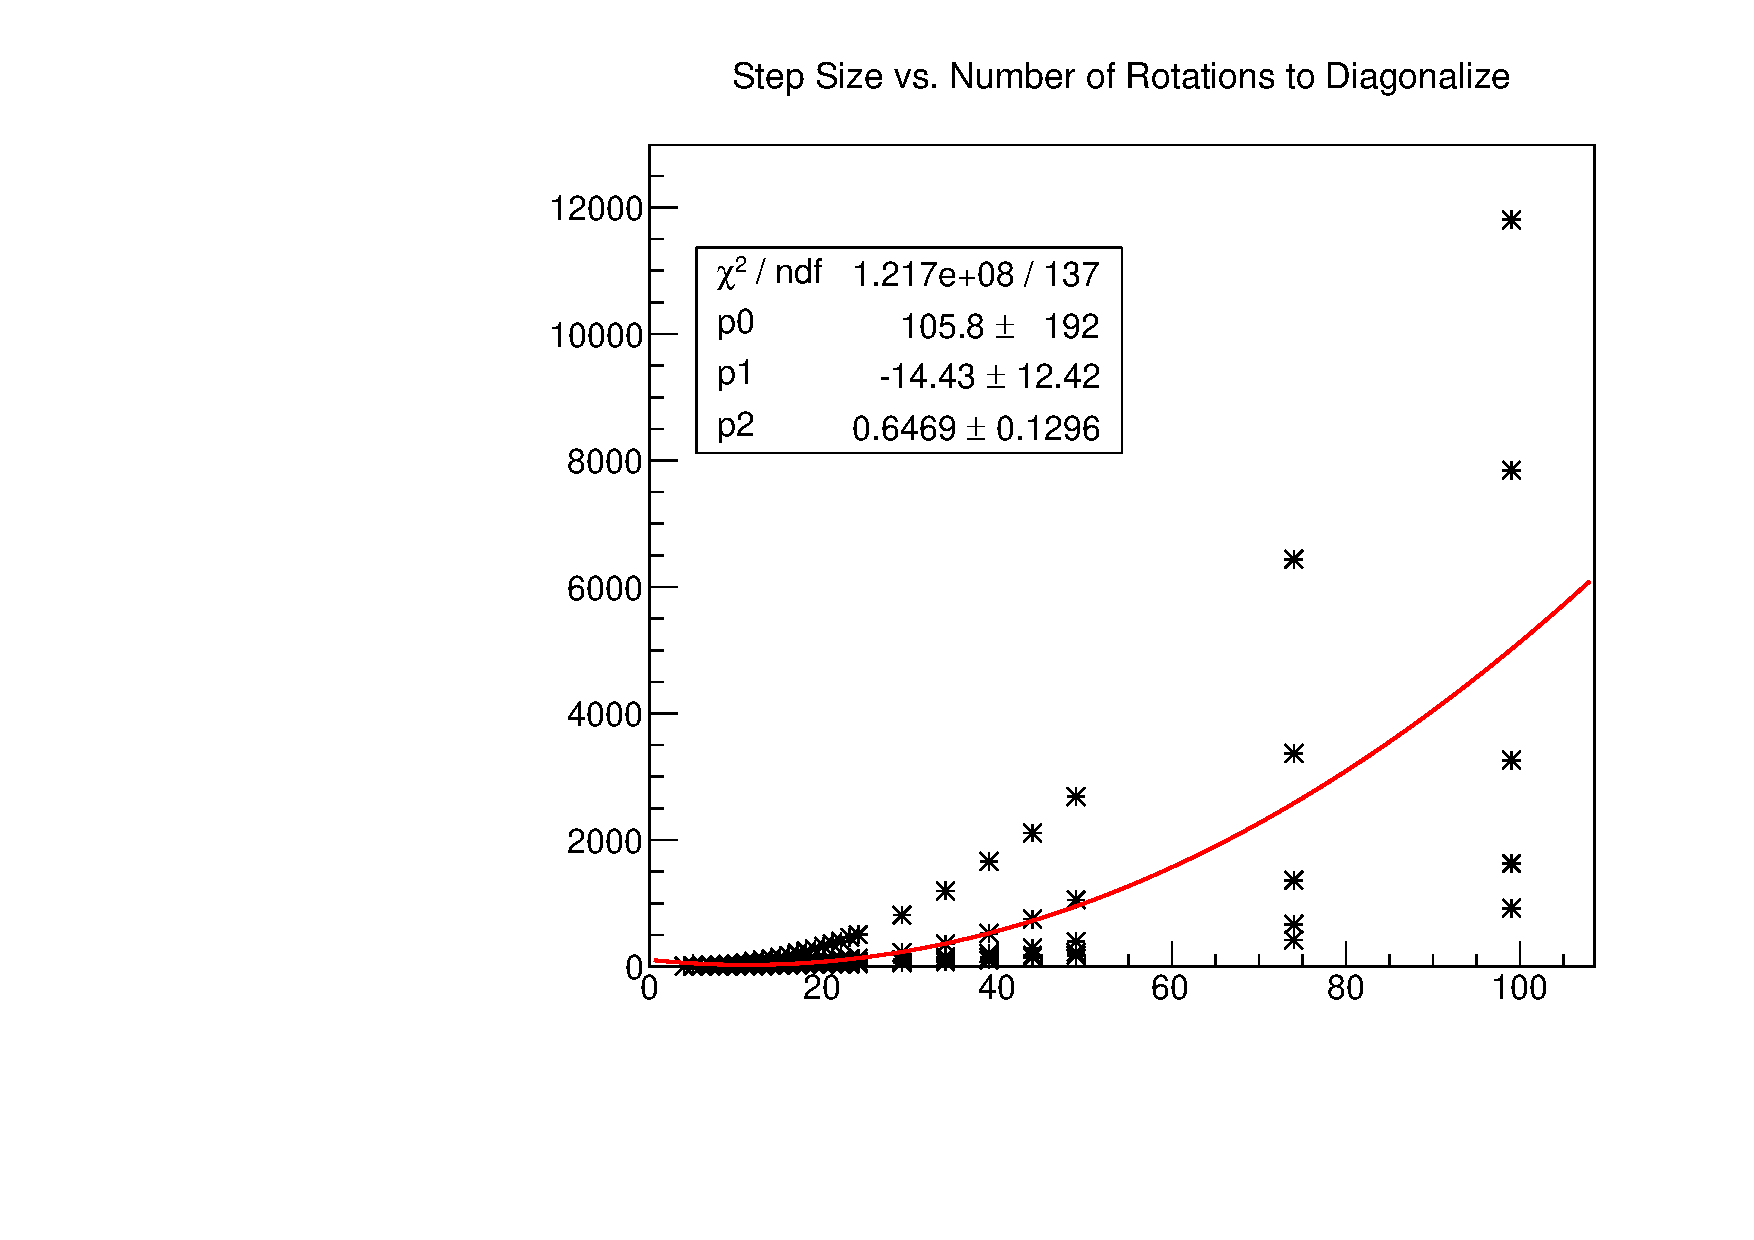
\includegraphics[width=0.45\textwidth]{plots/stepvrot}
\end{subfigure}
\caption{The number of rotations required by the Jacobi algorithm to diagonalize matrices of a given dimension.}
\end{center}
\end{figure}

\section{Results and Benchmarks}
\label{sec:results}
We begin by discussing the solution to the single-electron problem.  The ground state solutions are shown in Fig. 2, the 1st excited state in Fig 3, and the 2nd excited state in Fig 4.  We see in all cases of that the eigenvalues (energy) do indeed converge to about what we would expect (the first three ground state energies should be 3, 7, and 11) [4], even over very few numbers of steps.  We also see that, as expected, the distribution falls off quickly for larger radii.  In addition, we see nodes forming in the excited state distributions, as we expect.

\begin{figure}[h]
\label{fig:singlee}
\begin{center}
\begin{subfigure}
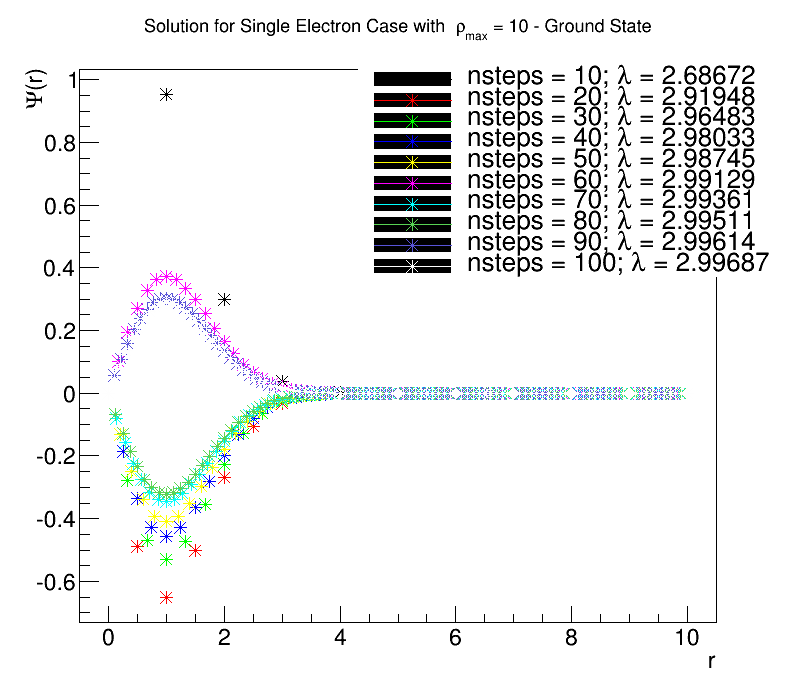
\includegraphics[width=0.45\textwidth]{plots/singlee10}
\end{subfigure}
\begin{subfigure}
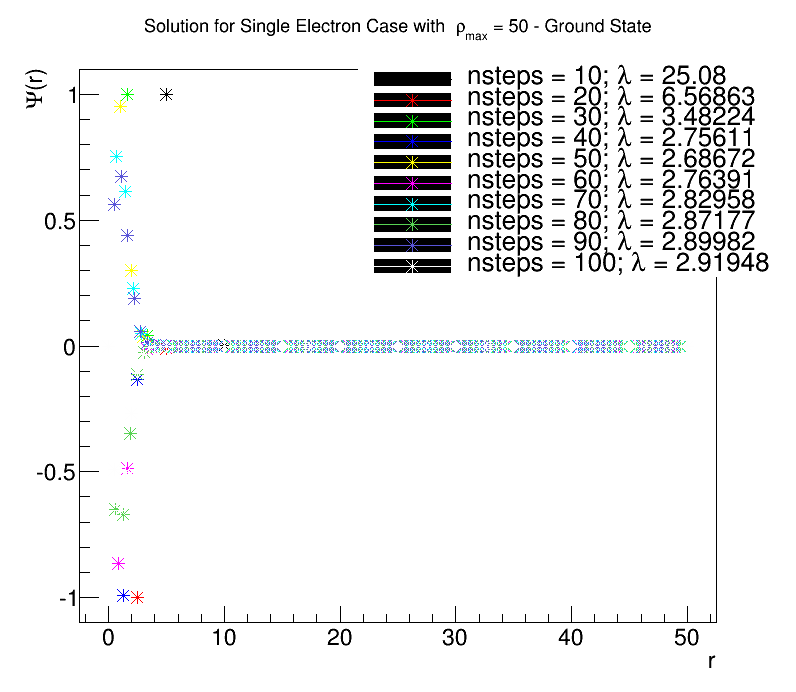
\includegraphics[width=0.45\textwidth]{plots/singlee50}
\end{subfigure}
\begin{subfigure}
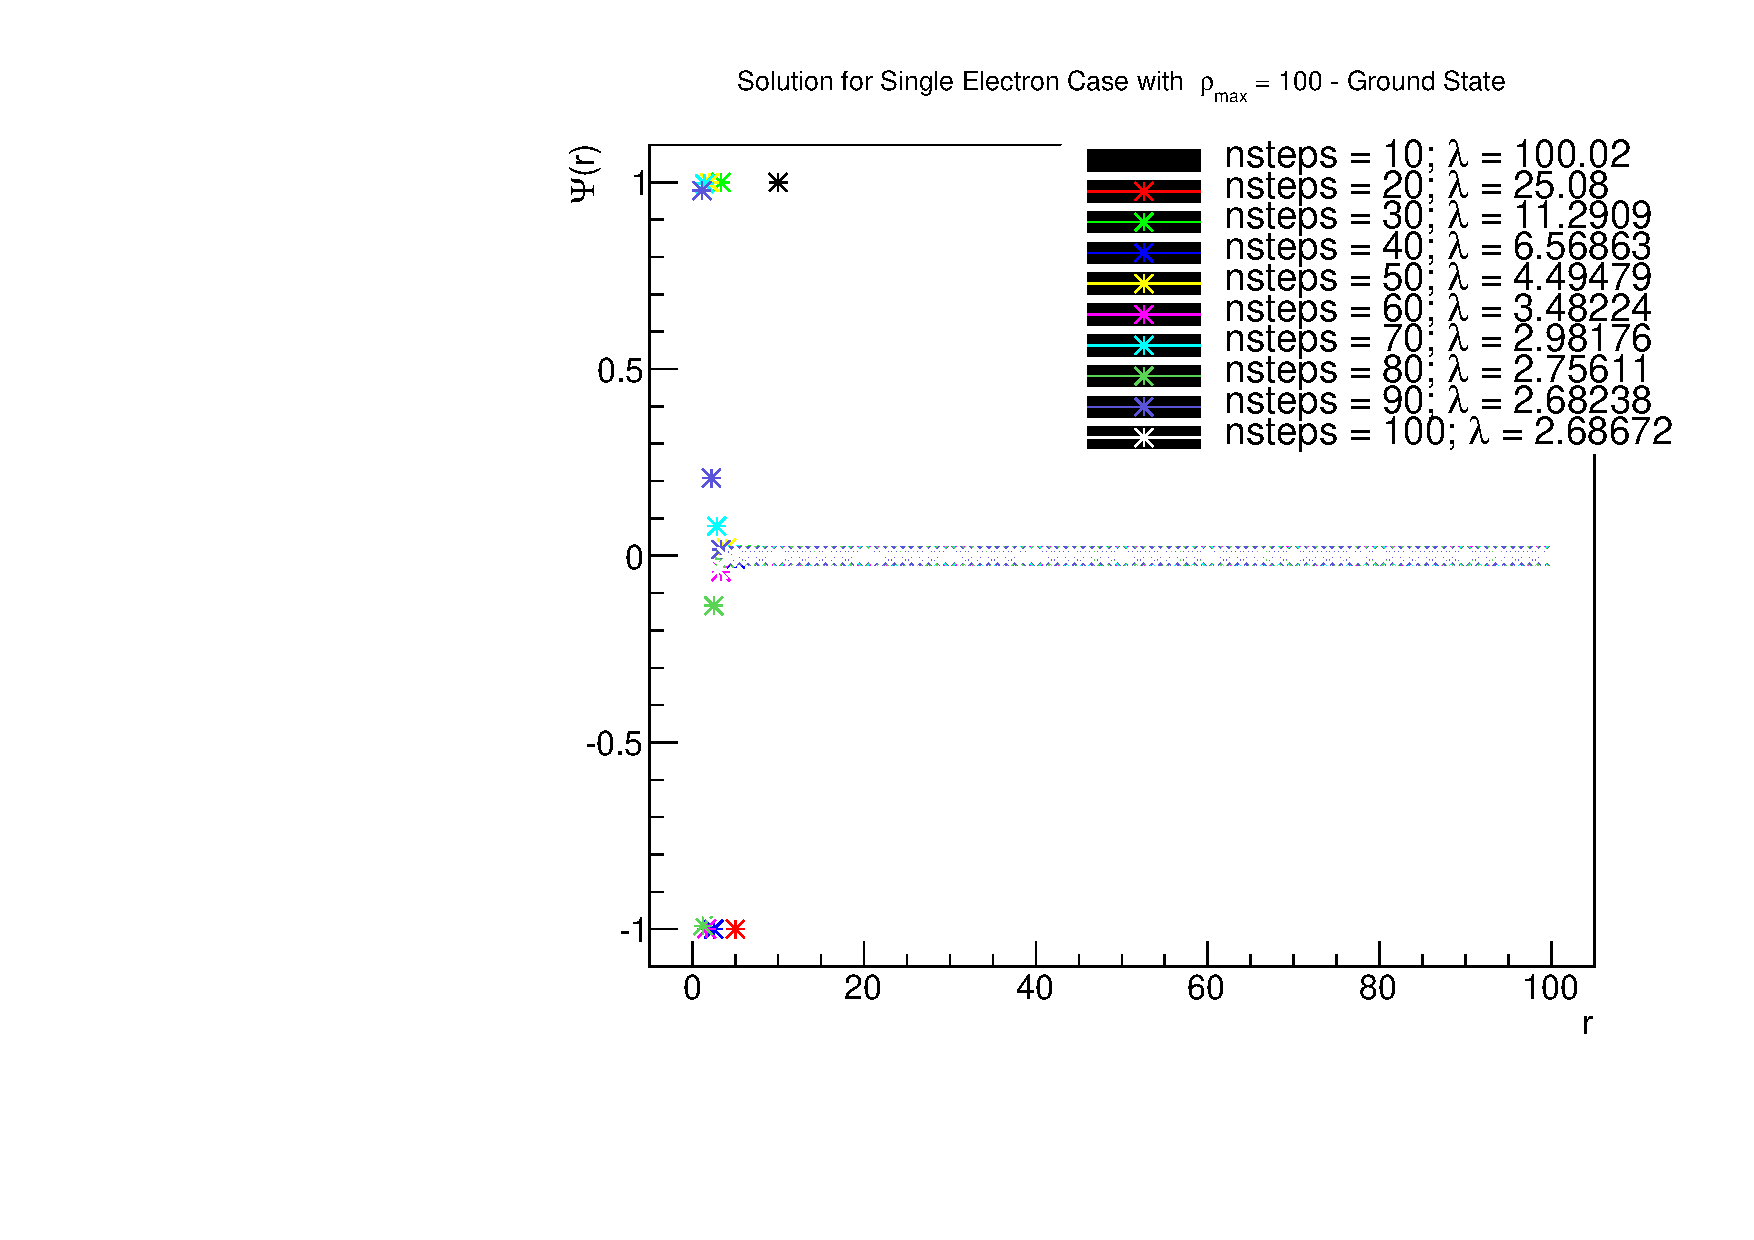
\includegraphics[width=0.45\textwidth]{plots/singlee100}
\end{subfigure}
\caption{Solutions for the single electron case for various values of $\rho_{max}$ in the ground state.}
\end{center}
\end{figure}

\begin{figure}[h]
\label{fig:singlee1}
\begin{center}
\begin{subfigure}
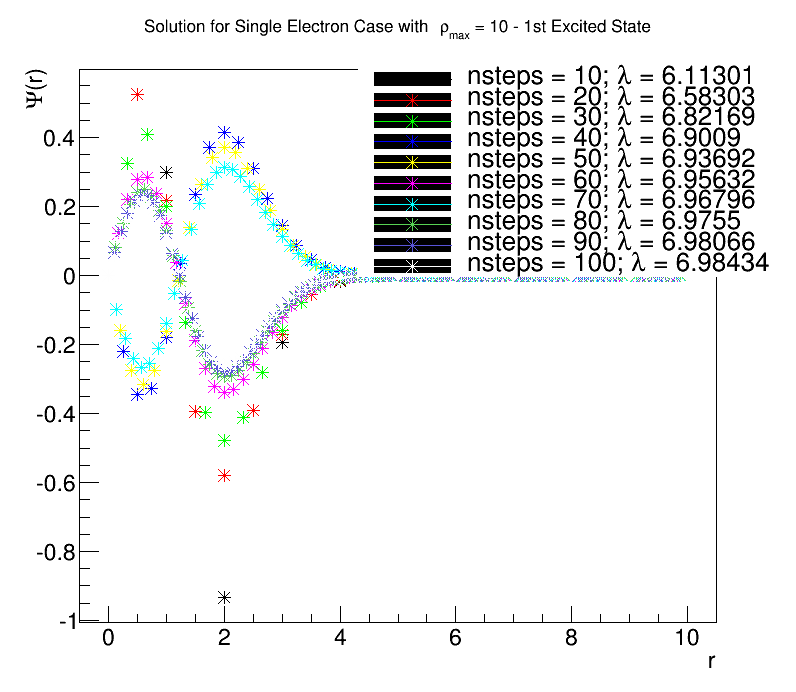
\includegraphics[width=0.45\textwidth]{plots/singlee101ststate}
\end{subfigure}
\begin{subfigure}
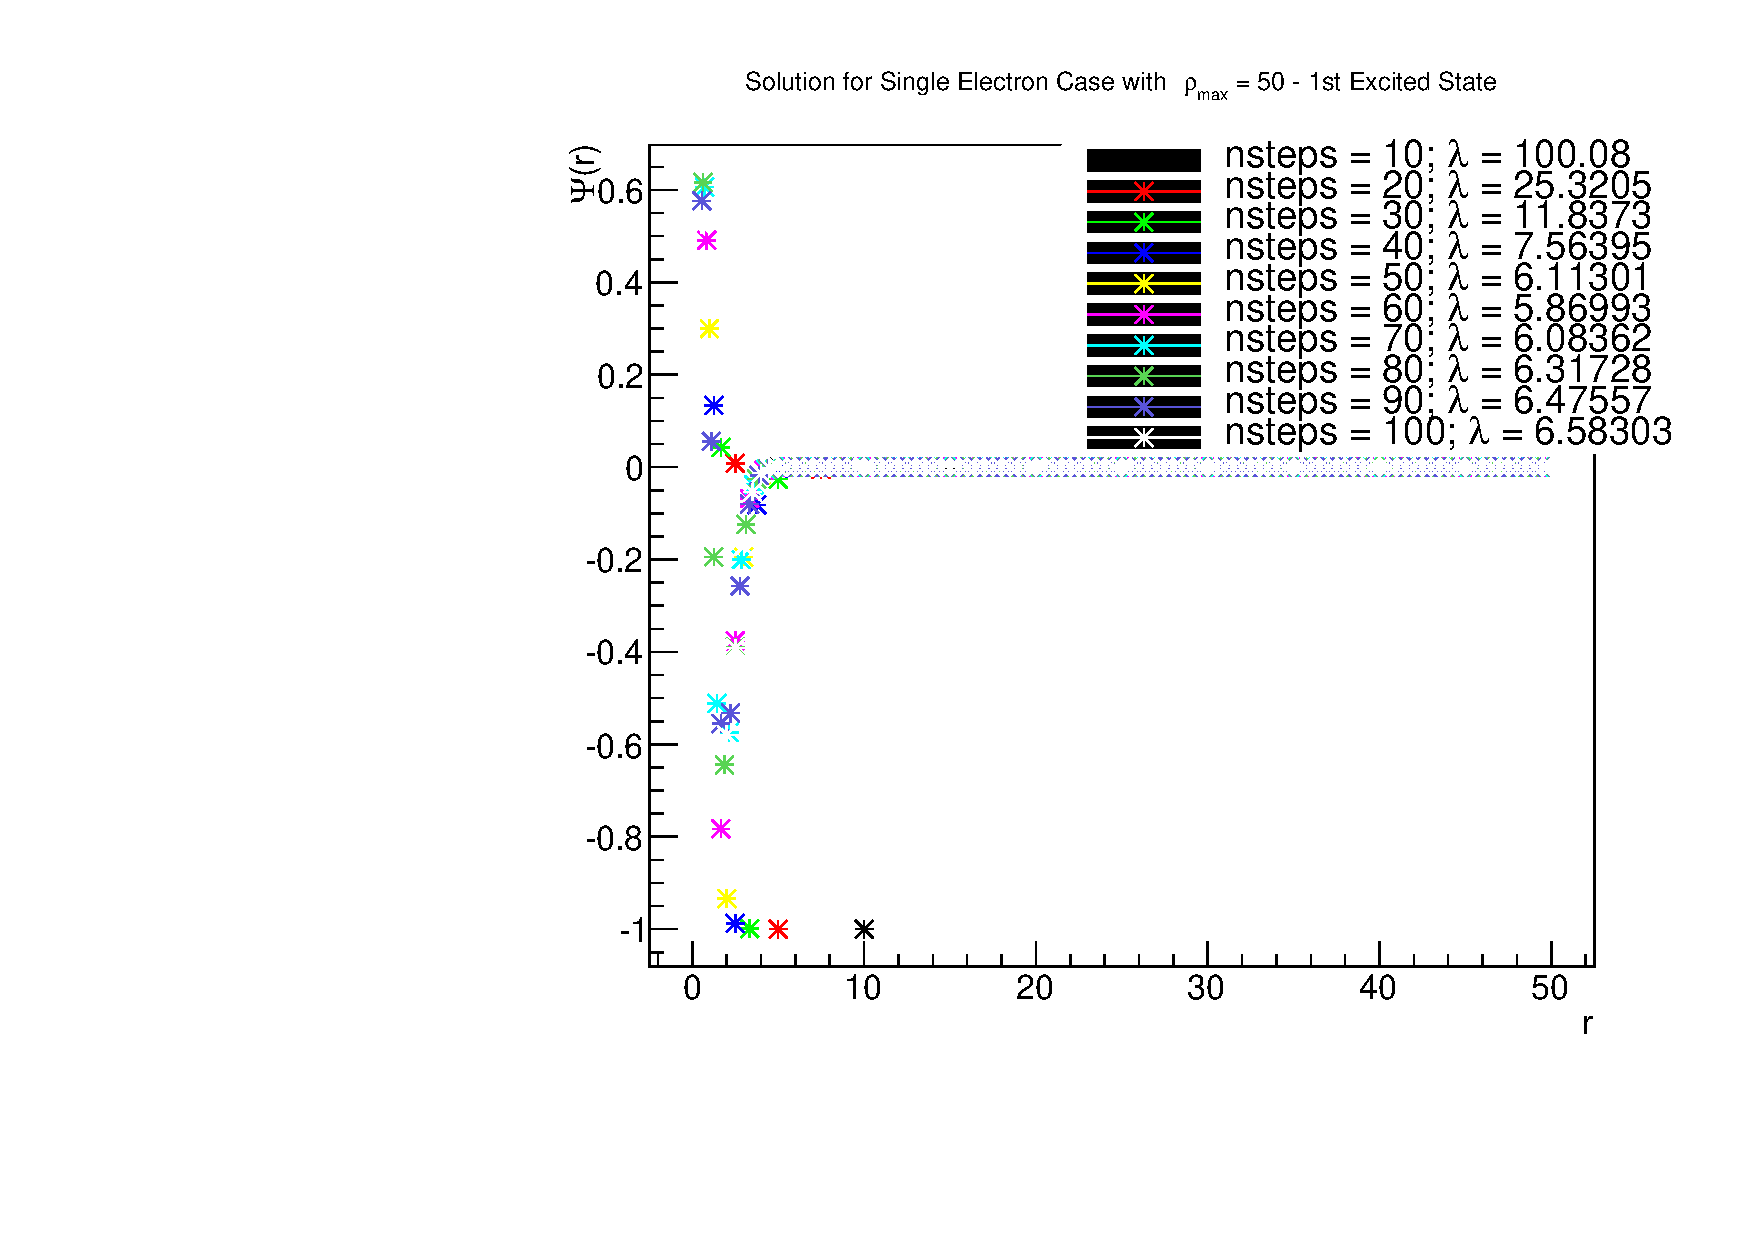
\includegraphics[width=0.45\textwidth]{plots/singlee501ststate}
\end{subfigure}
\begin{subfigure}
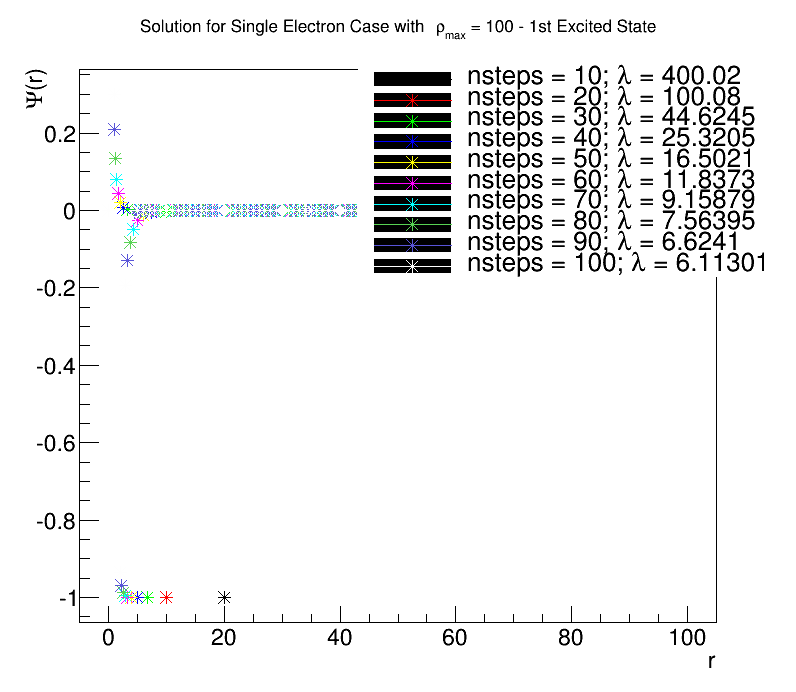
\includegraphics[width=0.45\textwidth]{plots/singlee1001ststate}
\end{subfigure}
\caption{Solutions for the single electron case for various values of $\rho_{max}$ in the 1st excited state.}
\end{center}
\end{figure}

\begin{figure}[h]
\label{fig:singlee2}
\begin{center}
\begin{subfigure}
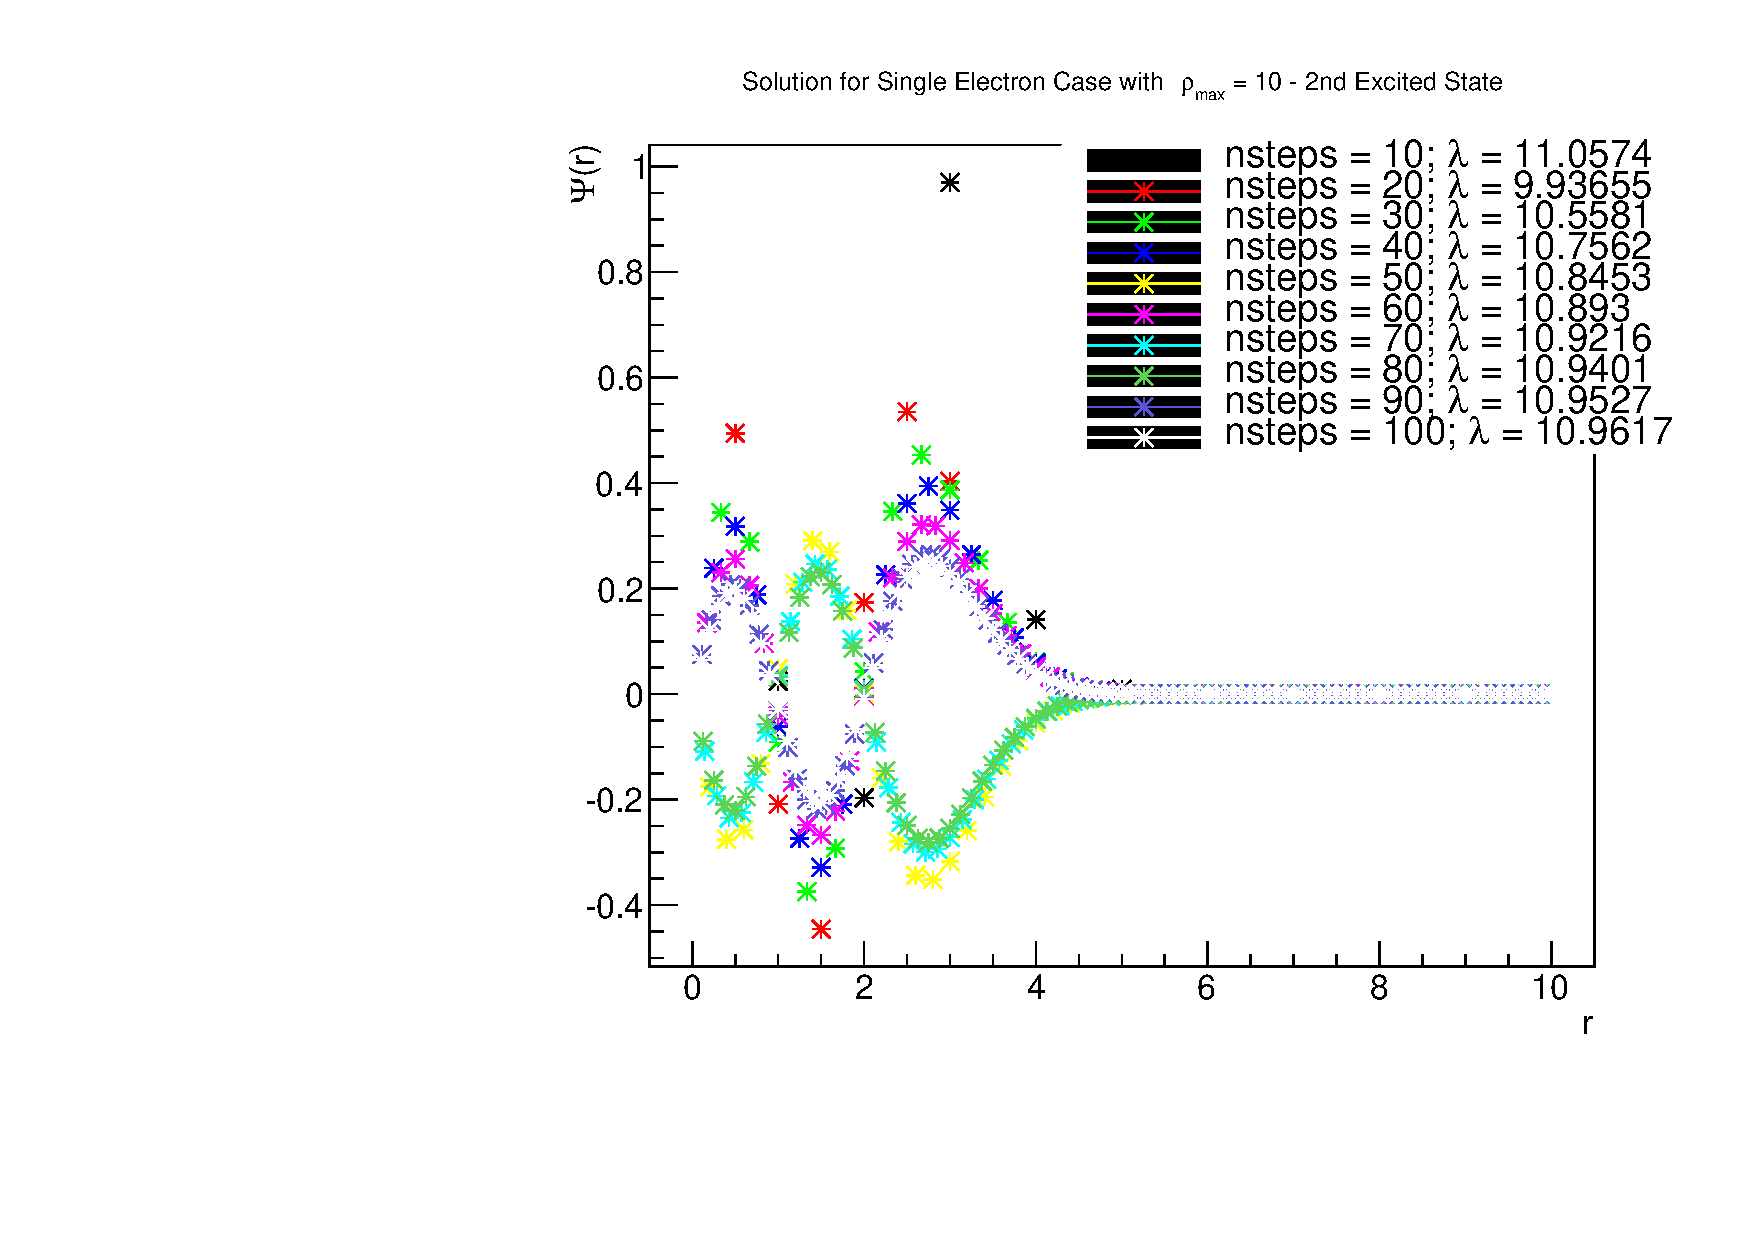
\includegraphics[width=0.45\textwidth]{plots/singlee102ndstate}
\end{subfigure}
\begin{subfigure}
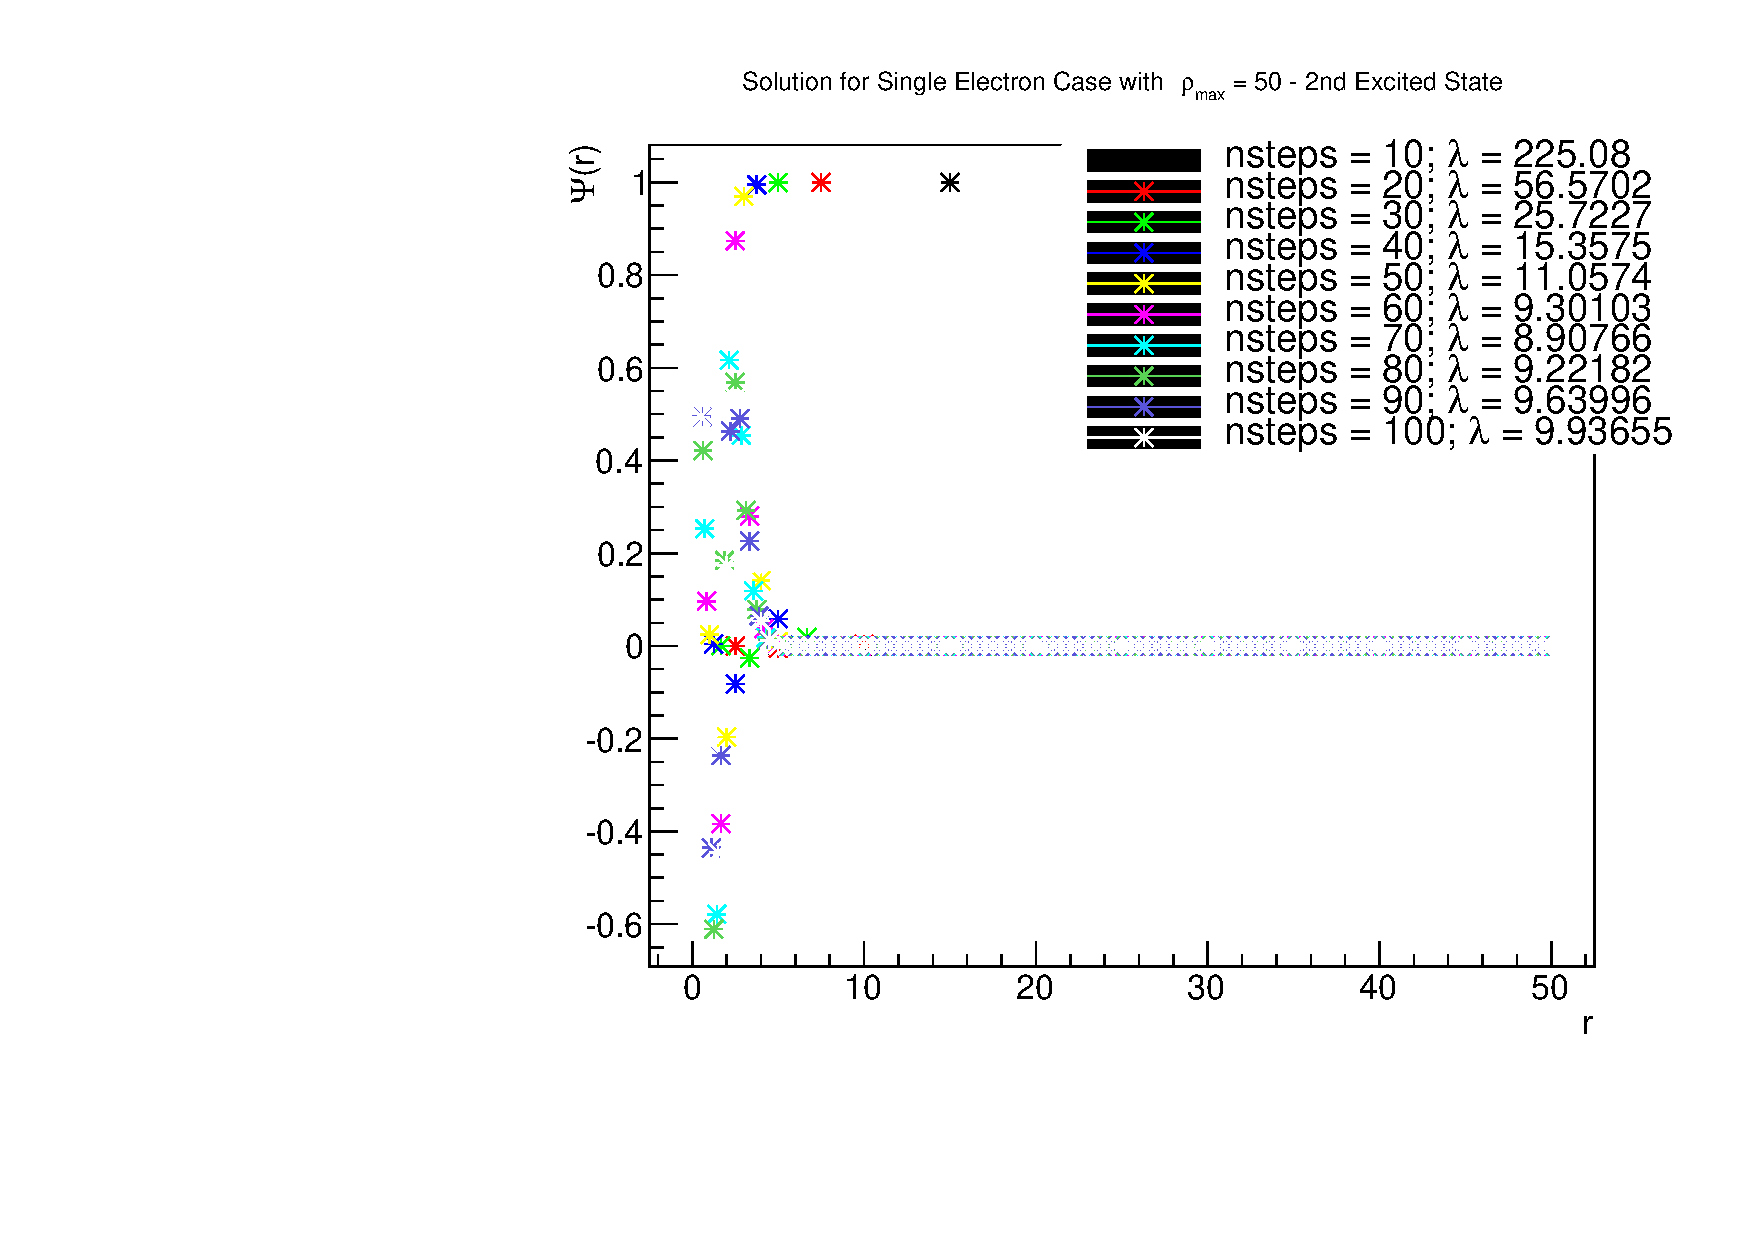
\includegraphics[width=0.45\textwidth]{plots/singlee502ndstate}
\end{subfigure}
\begin{subfigure}
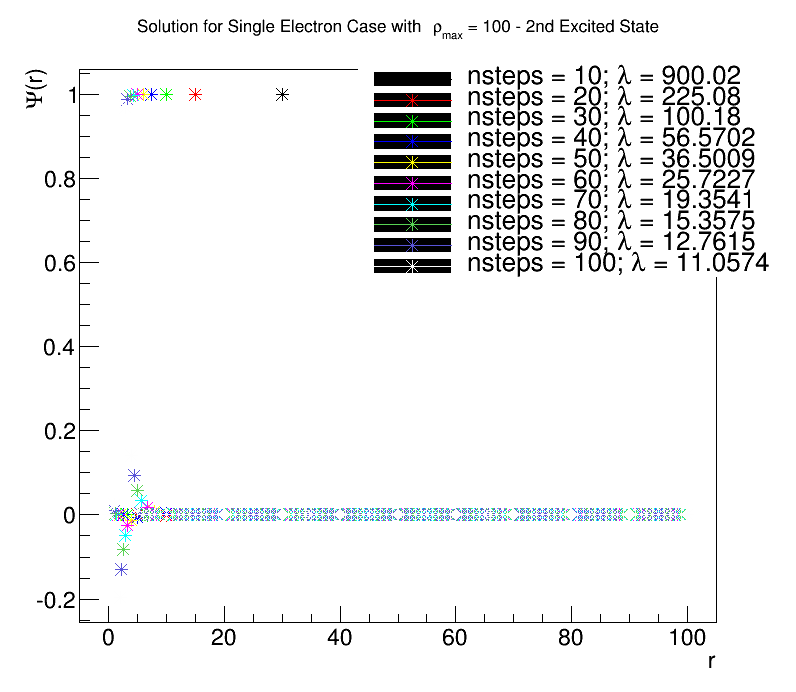
\includegraphics[width=0.45\textwidth]{plots/singlee1002ndstate}
\end{subfigure}
\caption{Solutions for the single electron case for various values of $\rho_{max}$ in the 2nd excited state.}
\end{center}
\end{figure}

\\\indent The analysis of the 2-electron problem is more involved, as we have multiple values of $\omega_{r}$, interacting and non-interacting cases, and multiple values of $\rho_{max}$.  These plots are shown in Figures 5-19.  As with the single electron, we see that, in all variations, the eigenvalues converge to some finite quantity with increasing numbers of steps.  We also see nodes appearing for excited states, and that the distribution drops off quickly for larger values of $\rho_{max}$.  It appears that larger $\omega_{r}$ cause the distribution to fluctuate with greater frequency and become less stable near the origin.  We also notice that the interacting potential peaks farther from the origin than the non-interacting potential.  This makes sense because the electrons would try to be as far from each other within the well as possible, which will likely imply that they are farther from the origin than the non-interacting electrons.  The plots for $\omega_{r}=1.0$ in the non-interacting regime should be very similar to those from the single electron system.

\begin{figure}[h]
\label{fig:2ewr001}
\begin{center}
\begin{subfigure}
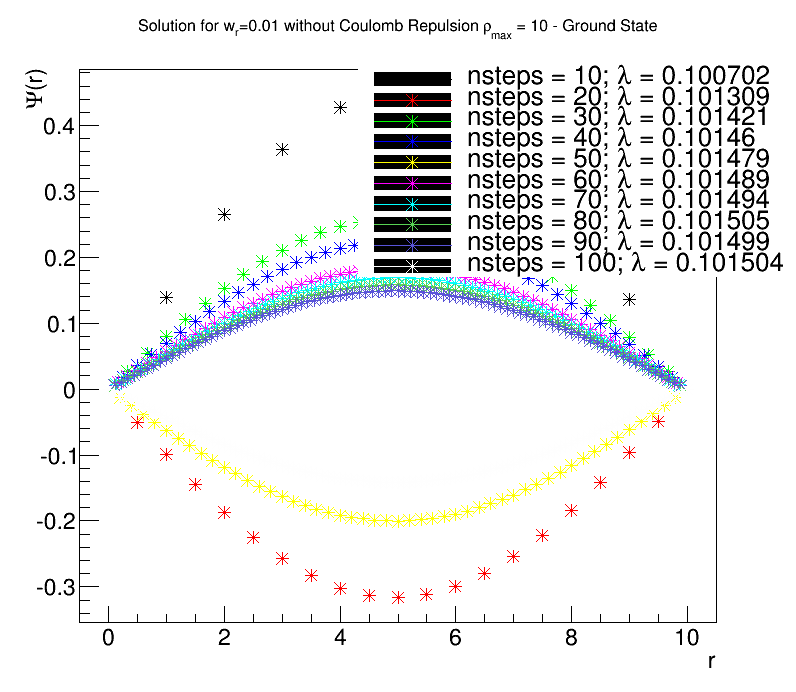
\includegraphics[width=0.45\textwidth]{plots/wr001NC10}
\end{subfigure}
\begin{subfigure}
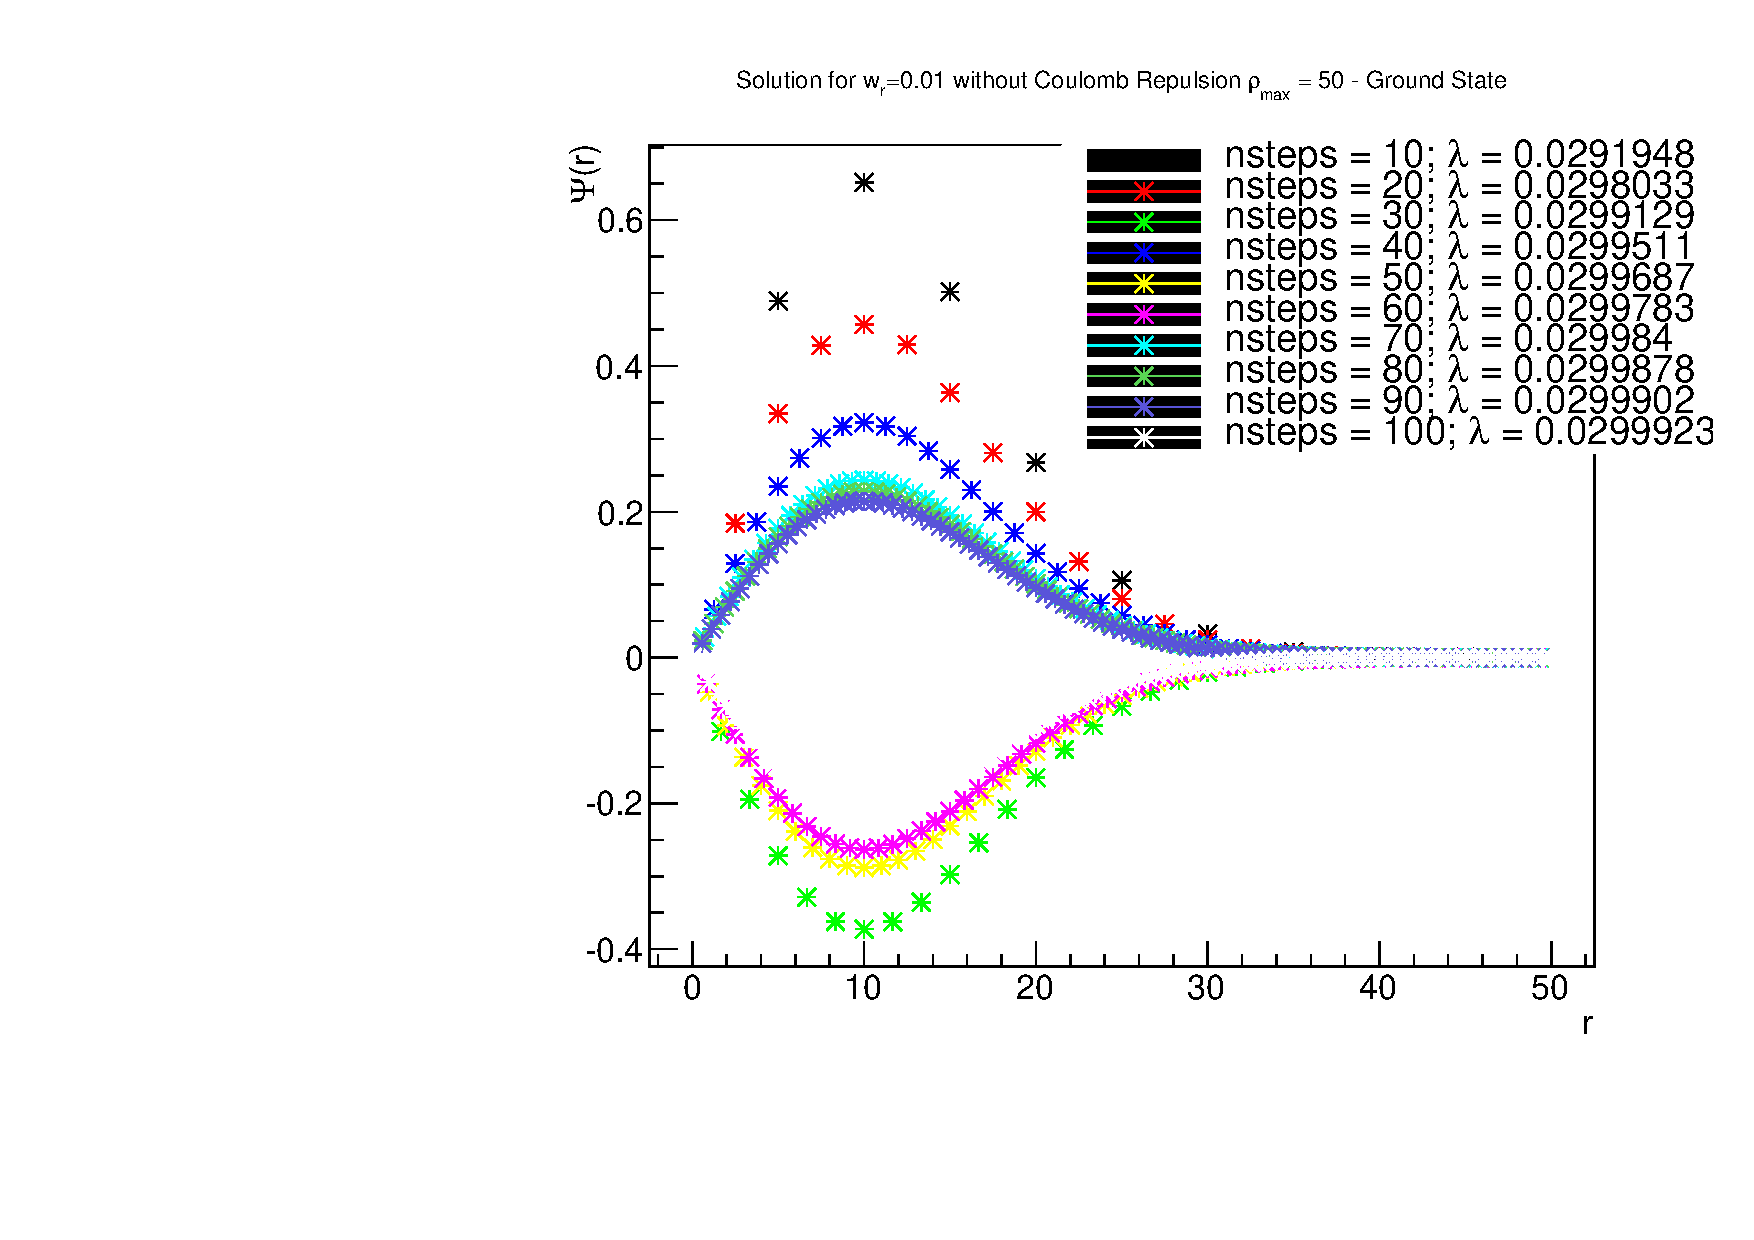
\includegraphics[width=0.45\textwidth]{plots/wr001NC50}
\end{subfigure}
\begin{subfigure}
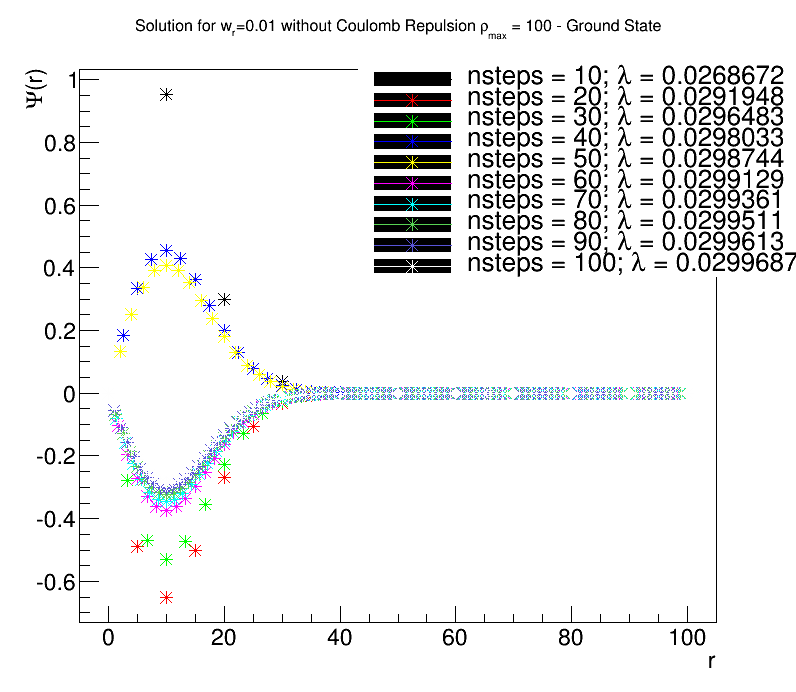
\includegraphics[width=0.45\textwidth]{plots/wr001NC100}
\end{subfigure}
\caption{Solutions for the non-interacting two-electron system for various values of $\rho_{max}$ in the ground state for $\omega_{r}=0.01$.}
\end{center}
\end{figure}

\begin{figure}[h]
\label{fig:2ewr05}
\begin{center}
\begin{subfigure}
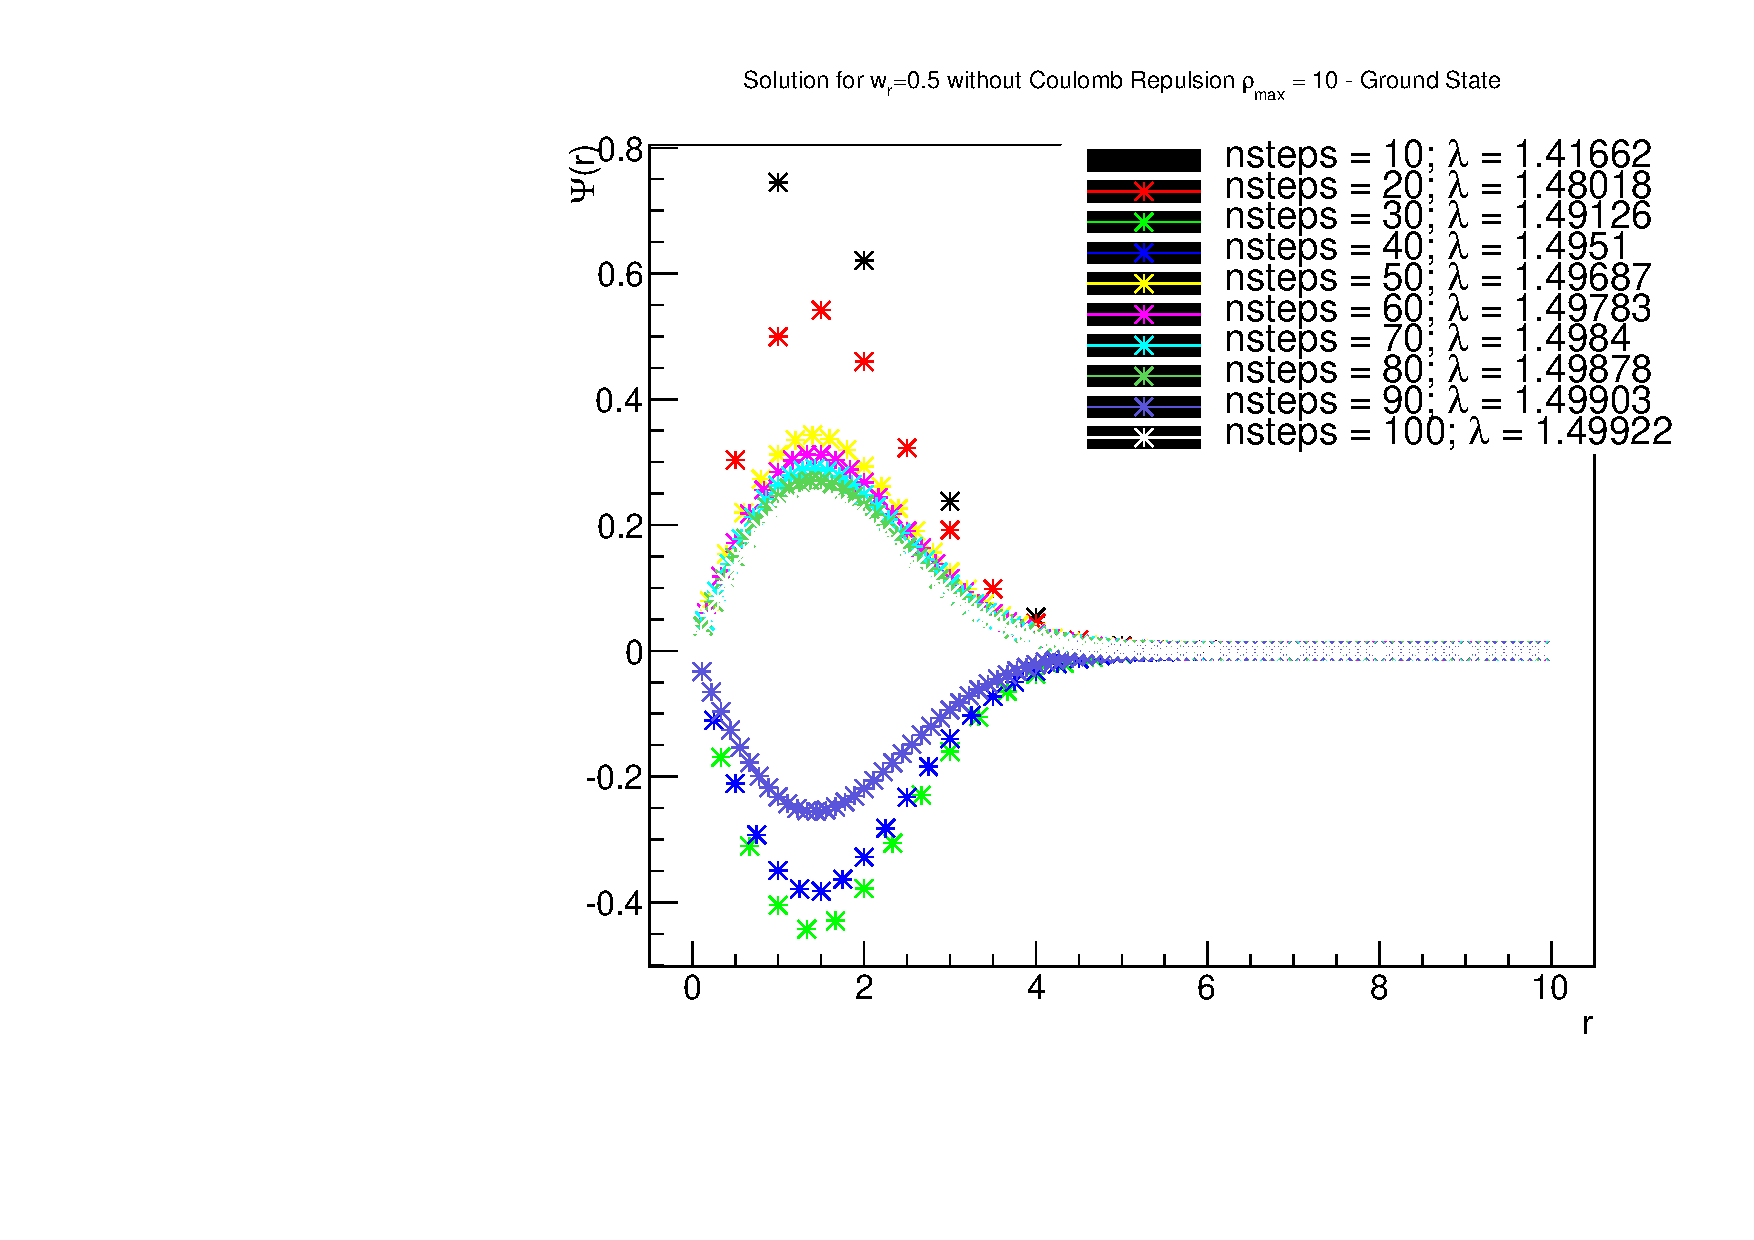
\includegraphics[width=0.45\textwidth]{plots/wr05NC10}
\end{subfigure}
\begin{subfigure}
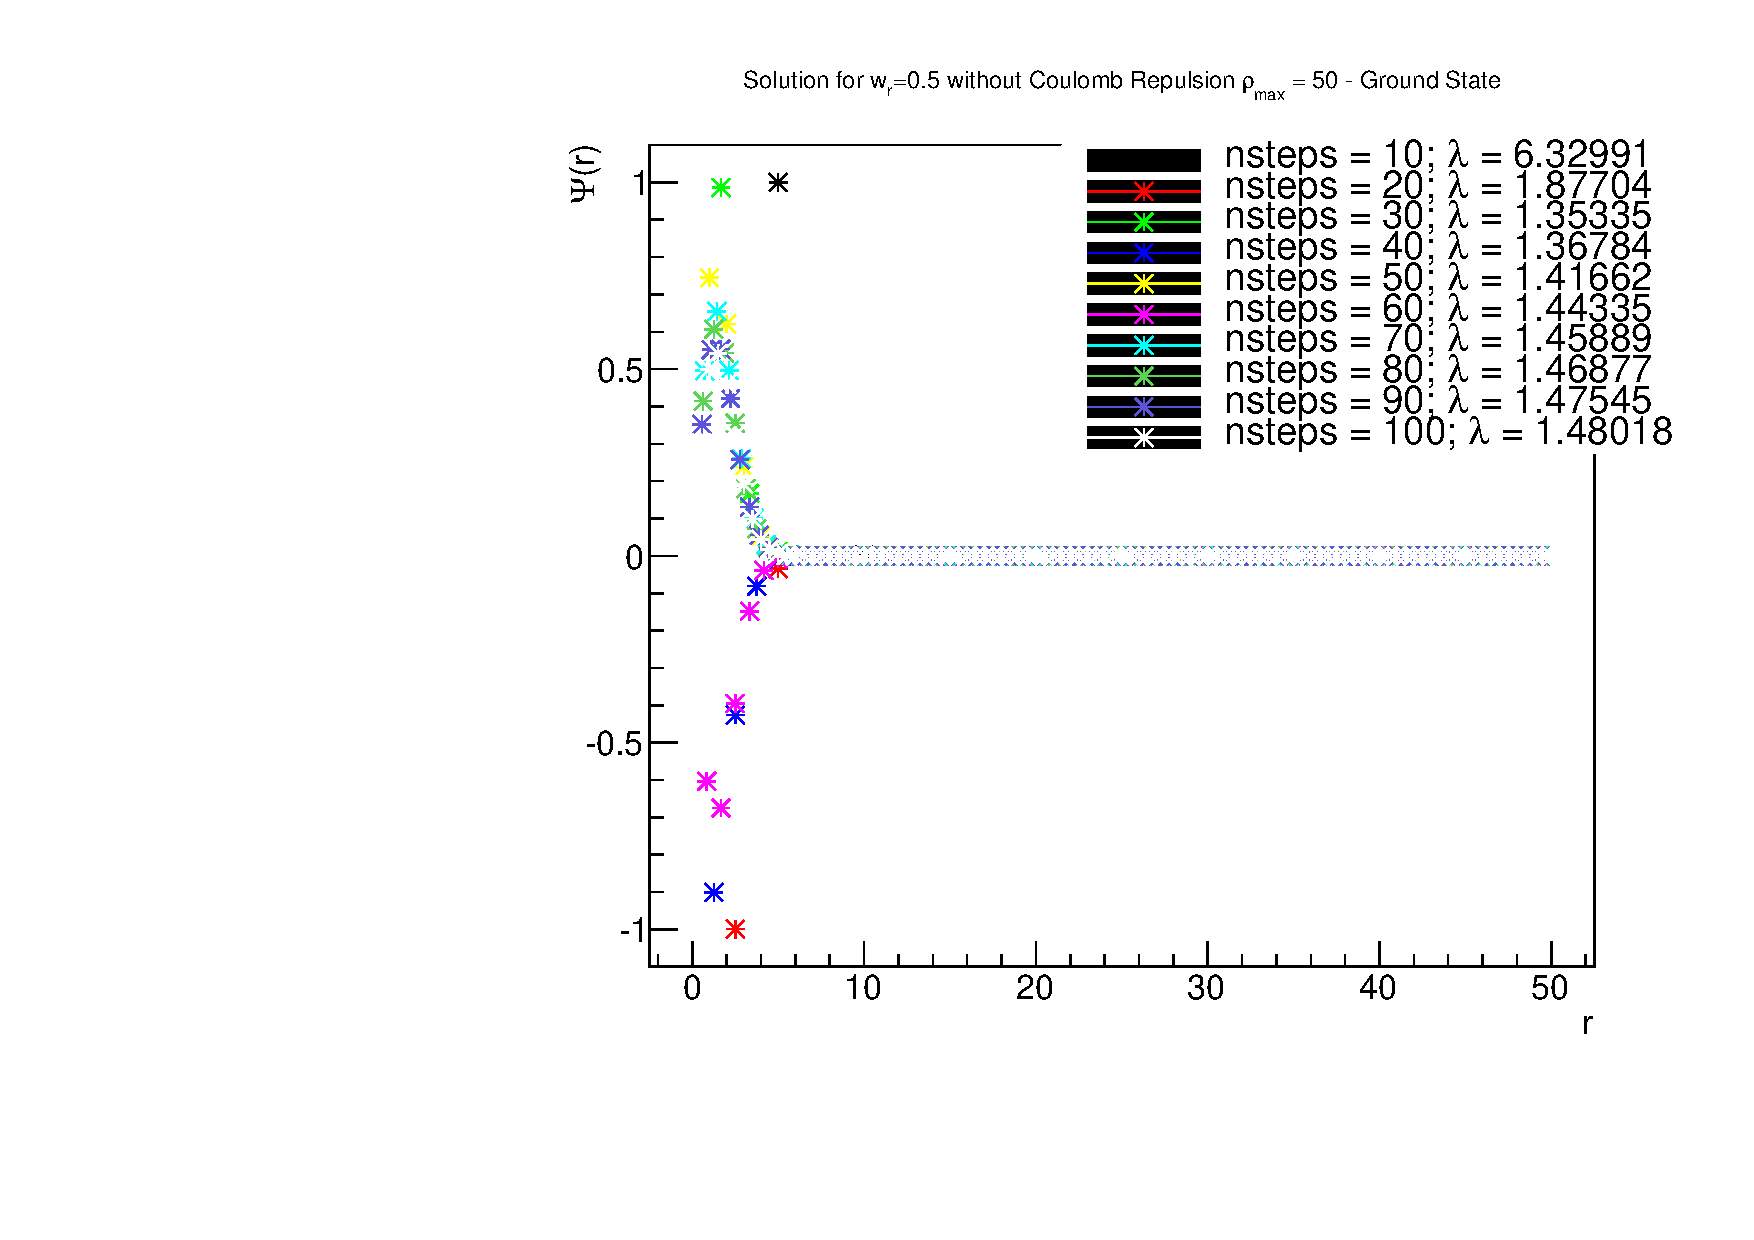
\includegraphics[width=0.45\textwidth]{plots/wr05NC50}
\end{subfigure}
\begin{subfigure}
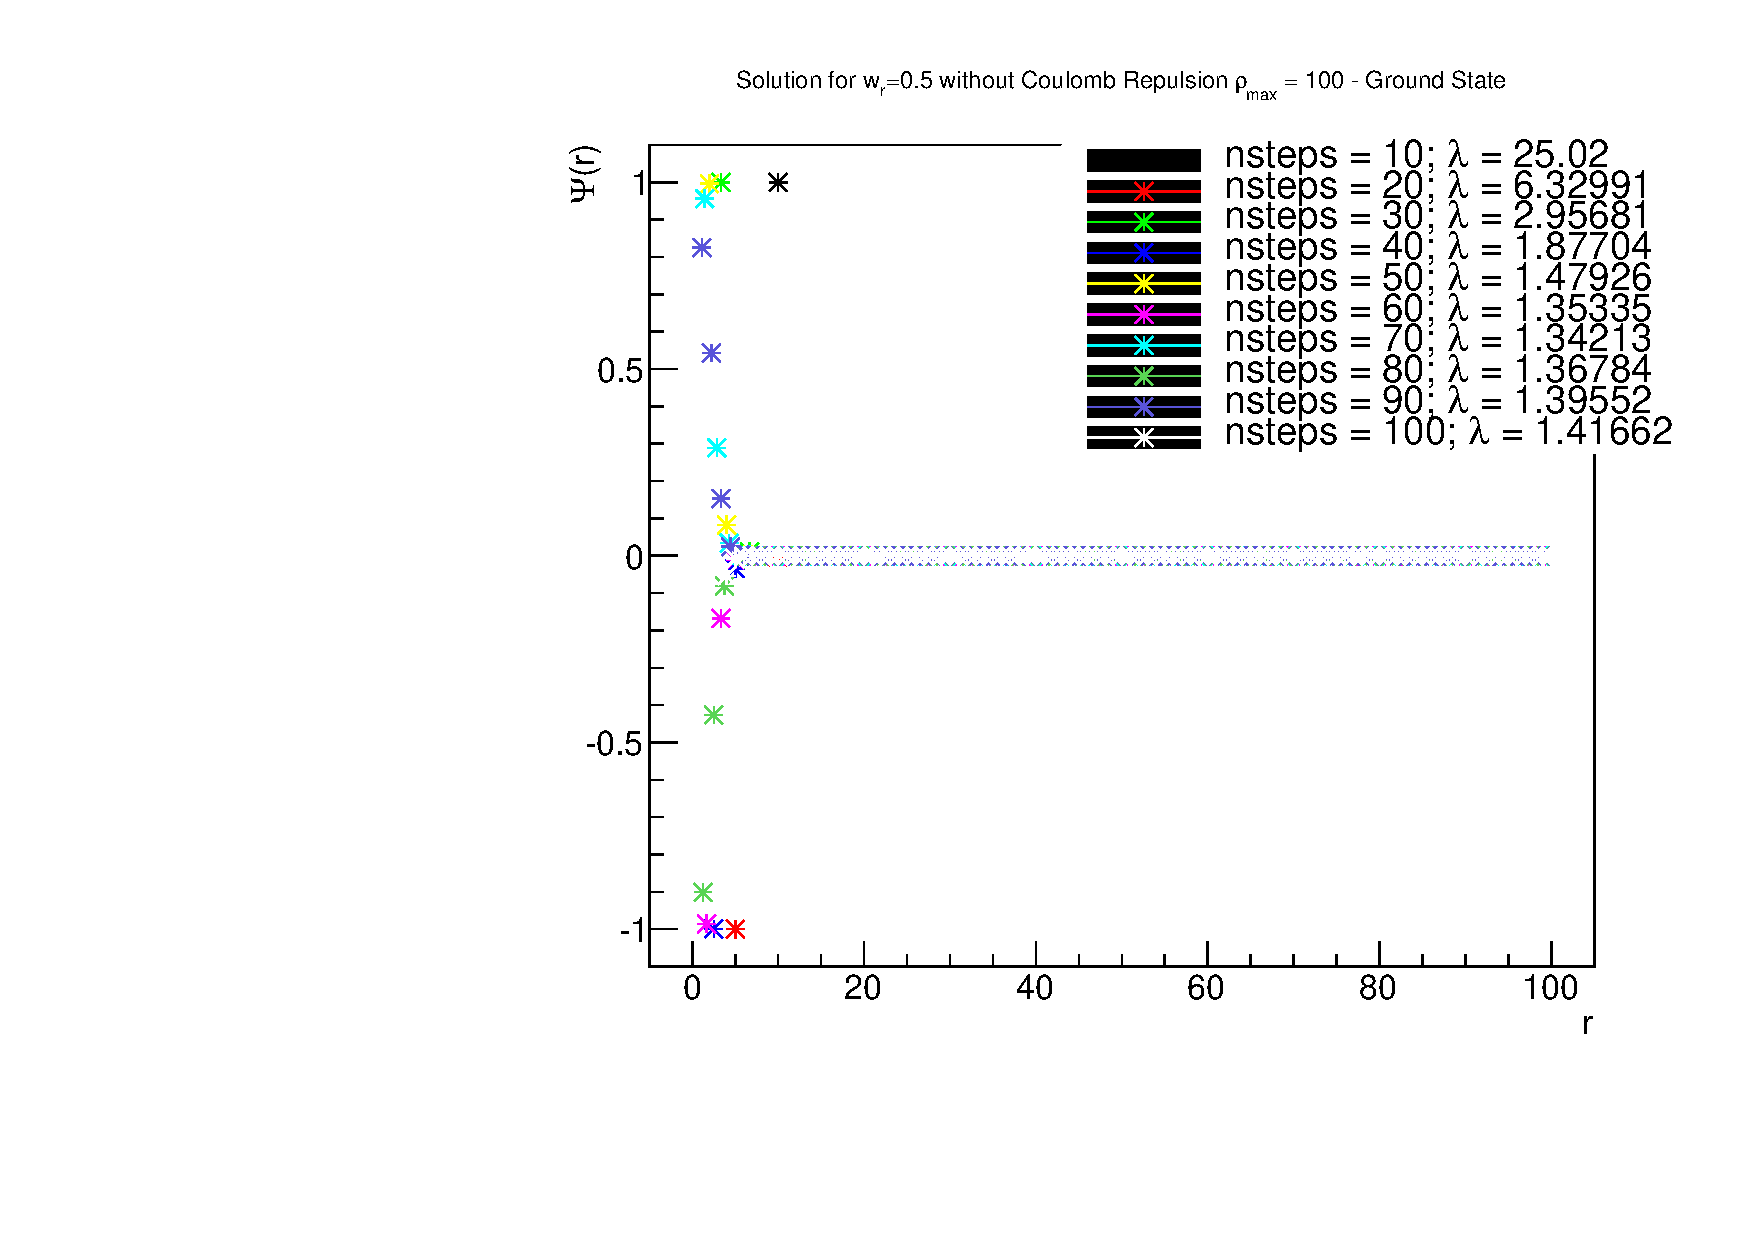
\includegraphics[width=0.45\textwidth]{plots/wr05NC100}
\end{subfigure}
\caption{Solutions for the non-interacting two-electron system for various values of $\rho_{max}$ in the ground state for $\omega_{r}=0.5$.}
\end{center}
\end{figure}

\begin{figure}[h]
\label{fig:2ewr1}
\begin{center}
\begin{subfigure}
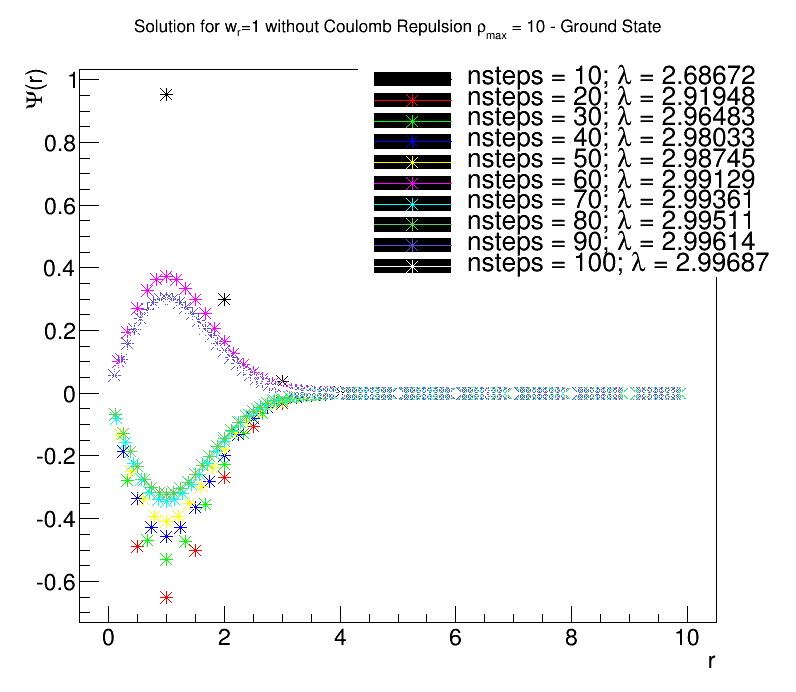
\includegraphics[width=0.45\textwidth]{plots/wr1NC10}
\end{subfigure}
\begin{subfigure}
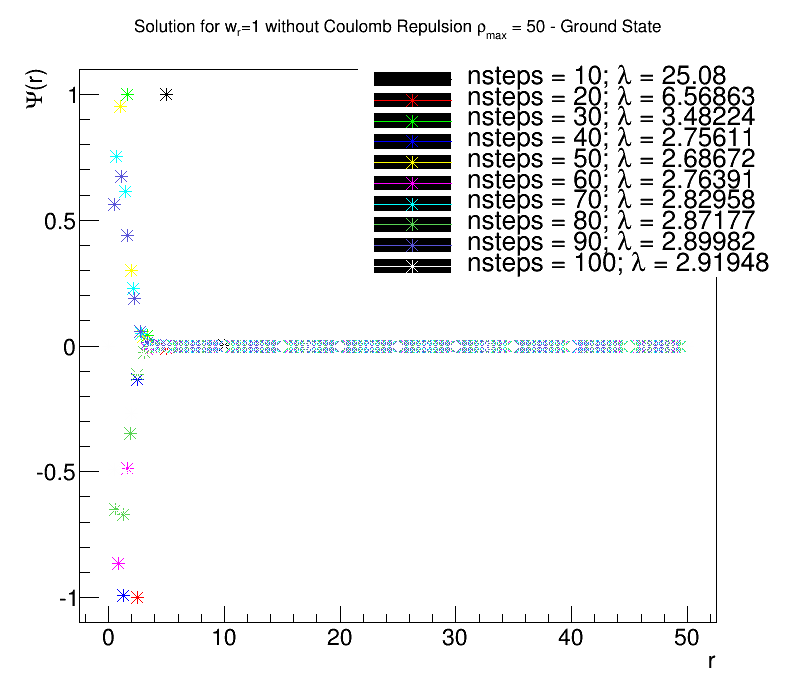
\includegraphics[width=0.45\textwidth]{plots/wr1NC50}
\end{subfigure}
\begin{subfigure}
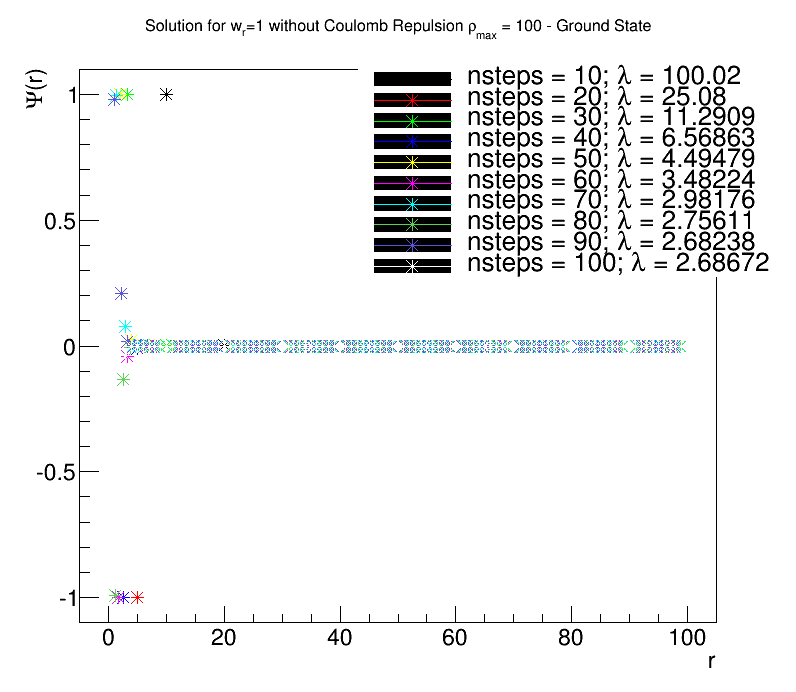
\includegraphics[width=0.45\textwidth]{plots/wr1NC100}
\end{subfigure}
\caption{Solutions for the non-interacting two-electron system for various values of $\rho_{max}$ in the ground state for $\omega_{r}=1.0$.}
\end{center}
\end{figure}

\begin{figure}[h]
\label{fig:2ewr5}
\begin{center}
\begin{subfigure}
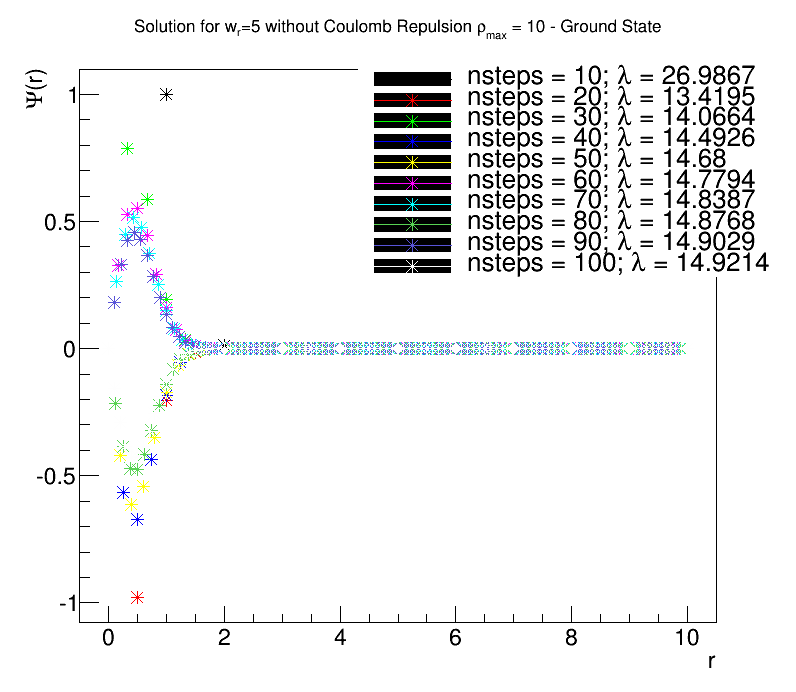
\includegraphics[width=0.45\textwidth]{plots/wr5NC10}
\end{subfigure}
\begin{subfigure}
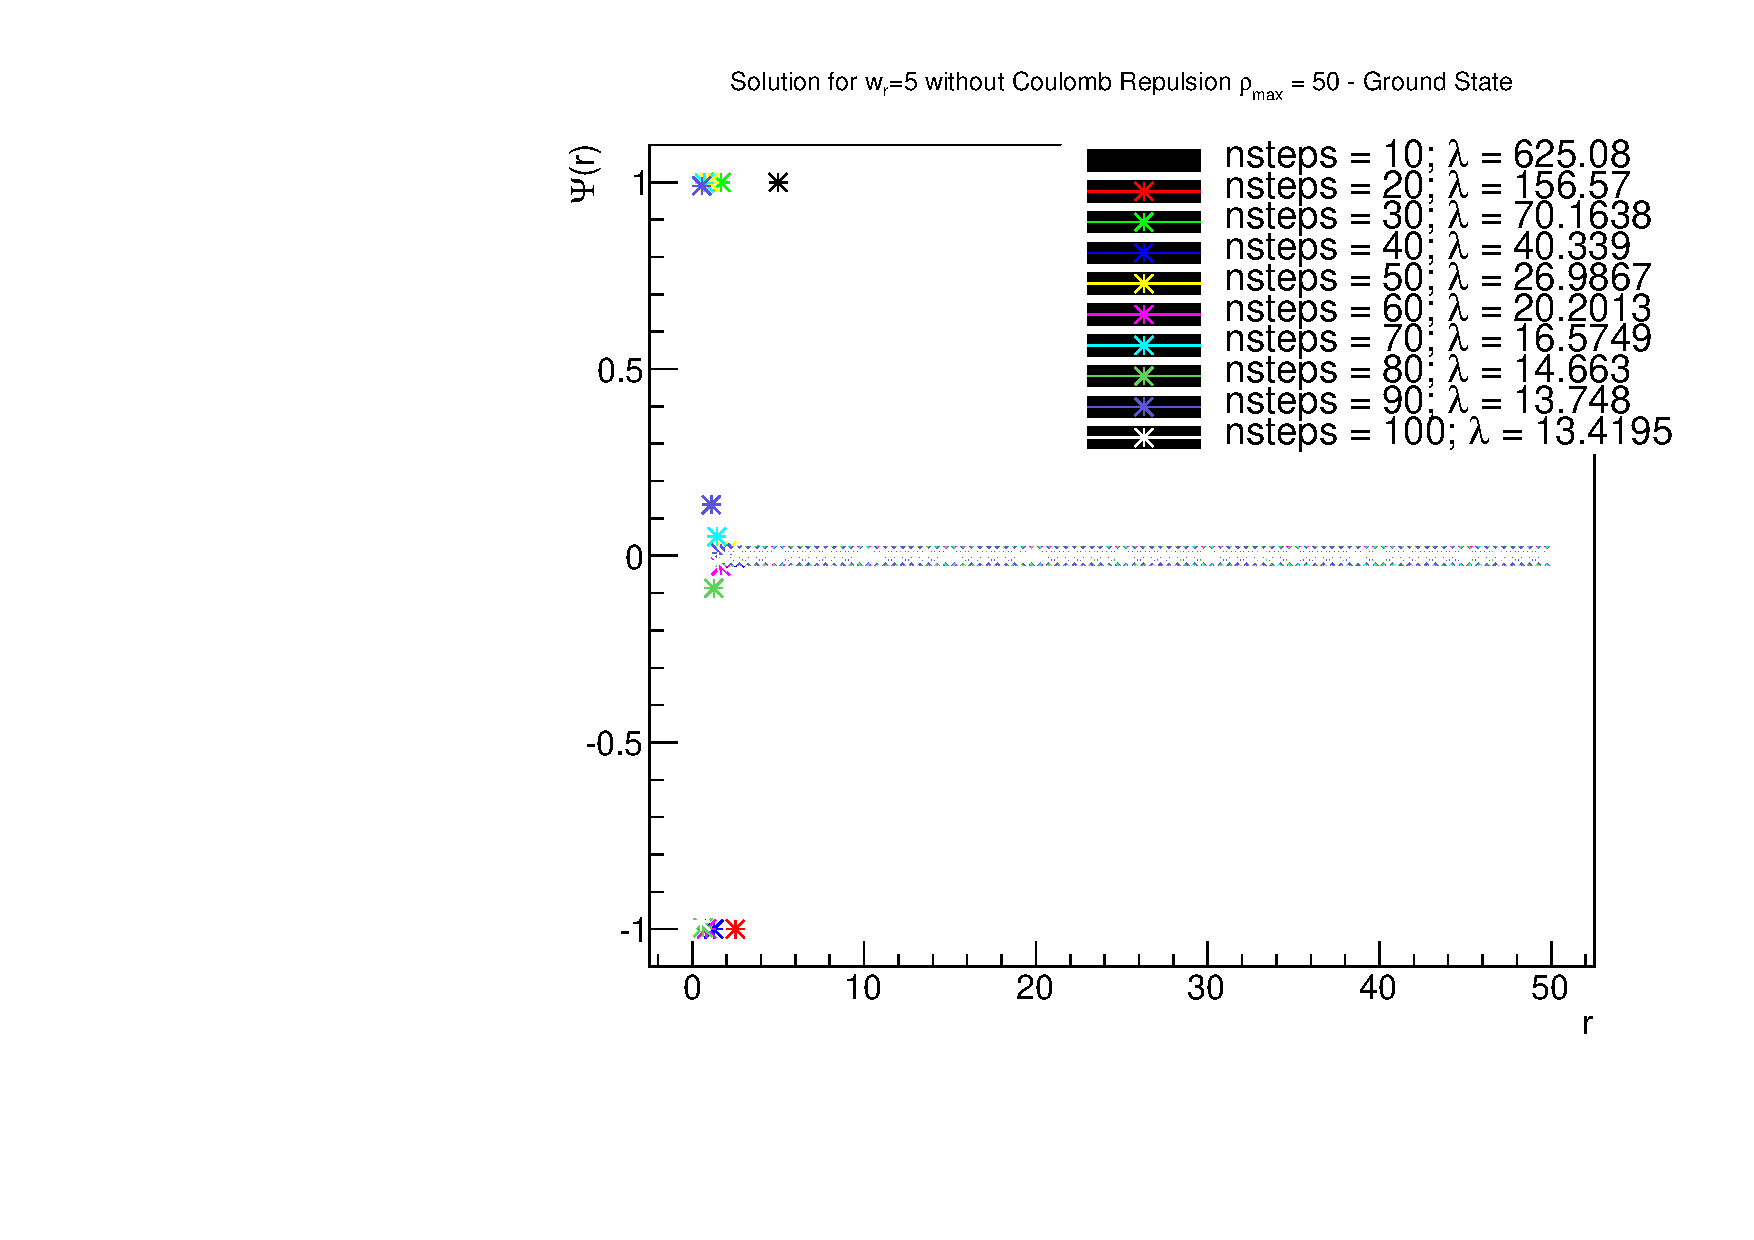
\includegraphics[width=0.45\textwidth]{plots/wr5NC50}
\end{subfigure}
\begin{subfigure}
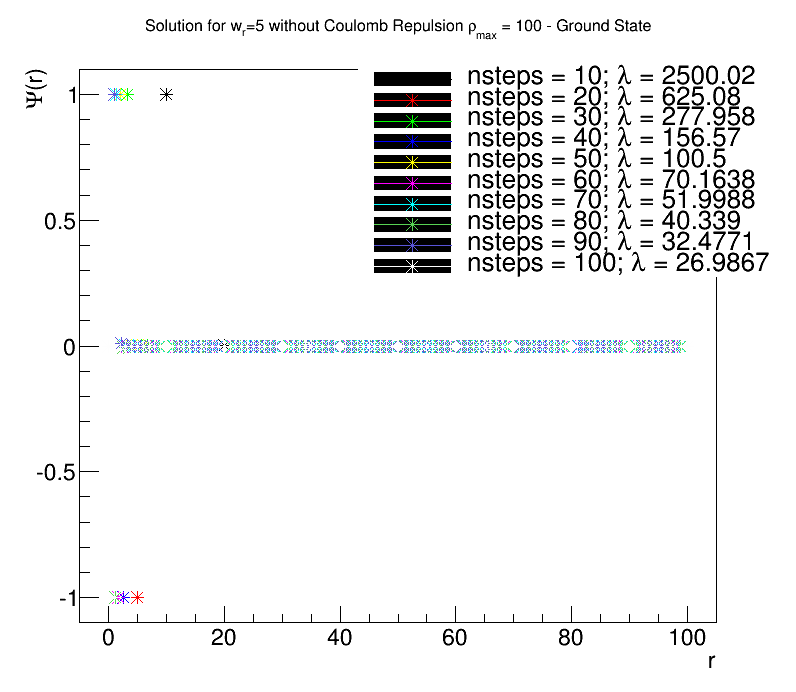
\includegraphics[width=0.45\textwidth]{plots/wr5NC100}
\end{subfigure}
\caption{Solutions for the non-interacting two-electron system for various values of $\rho_{max}$ in the ground state for $\omega_{r}=5.0$.}
\end{center}
\end{figure}

\begin{figure}[h]
\label{fig:2ewr001c}
\begin{center}
\begin{subfigure}
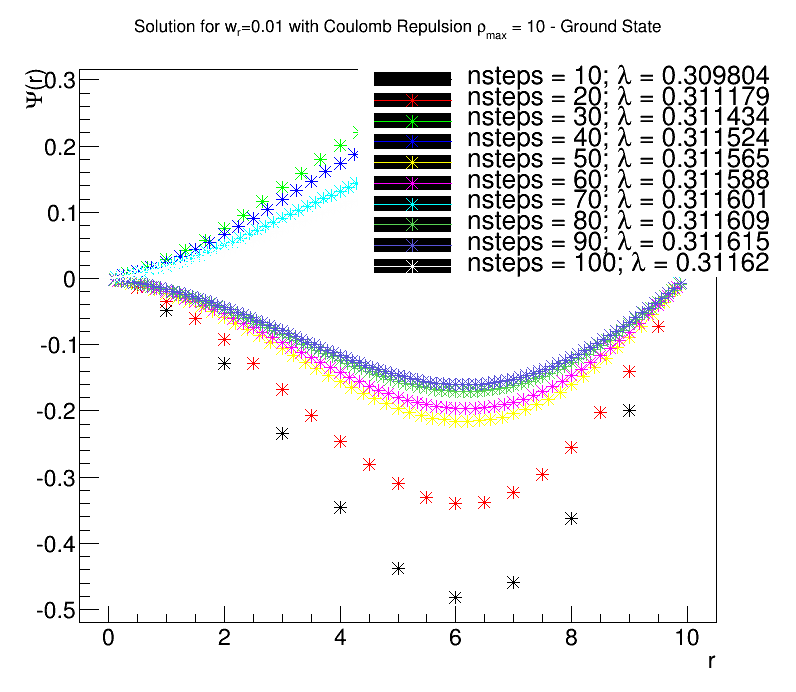
\includegraphics[width=0.45\textwidth]{plots/wr001C10}
\end{subfigure}
\begin{subfigure}
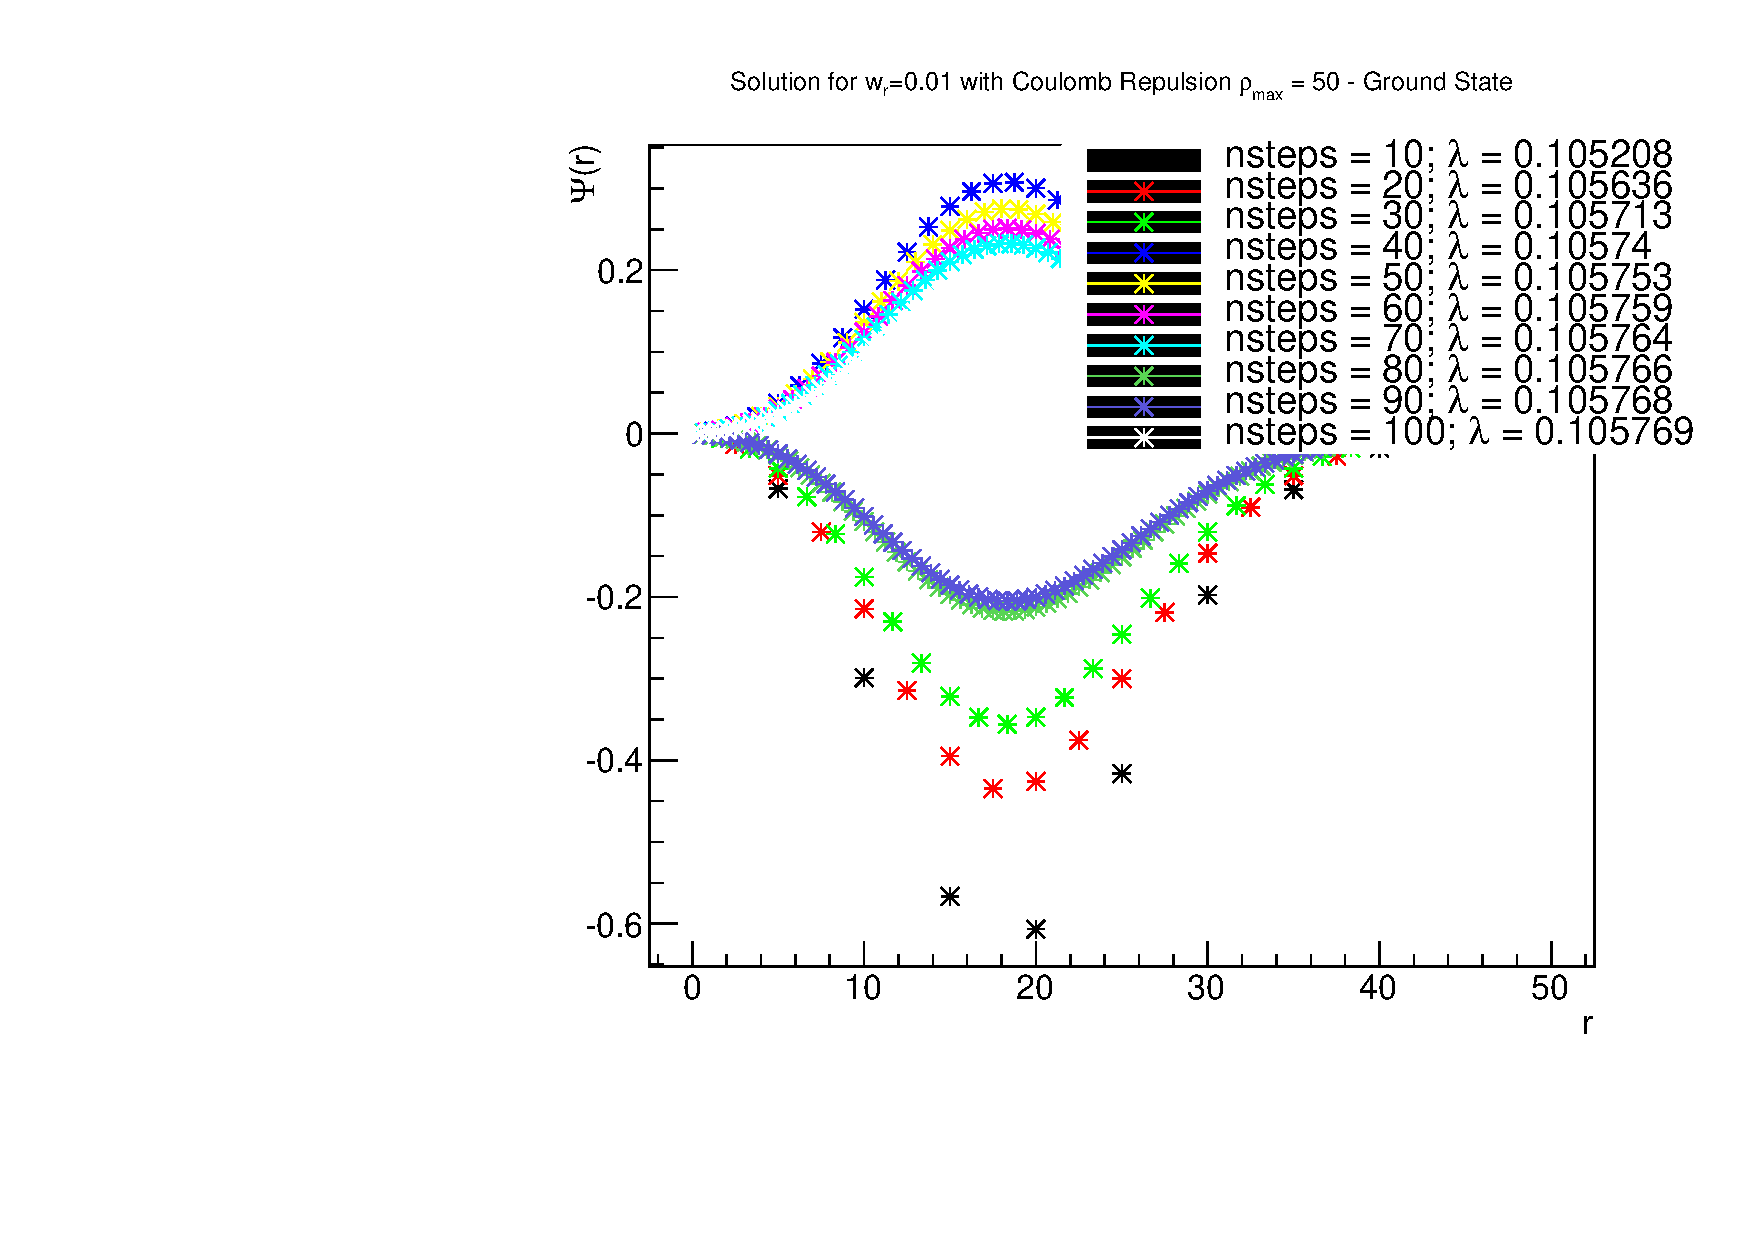
\includegraphics[width=0.45\textwidth]{plots/wr001C50}
\end{subfigure}
\begin{subfigure}
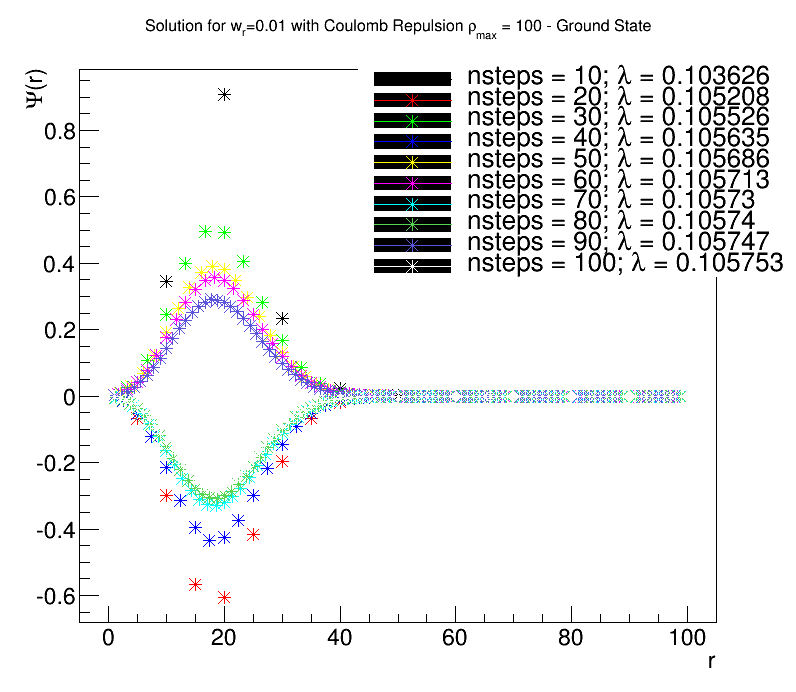
\includegraphics[width=0.45\textwidth]{plots/wr001C100}
\end{subfigure}
\caption{Solutions for the interacting two-electron system for various values of $\rho_{max}$ in the ground state for $\omega_{r}=0.01$.}
\end{center}
\end{figure}

\begin{figure}[h]
\label{fig:2ewr05c}
\begin{center}
\begin{subfigure}
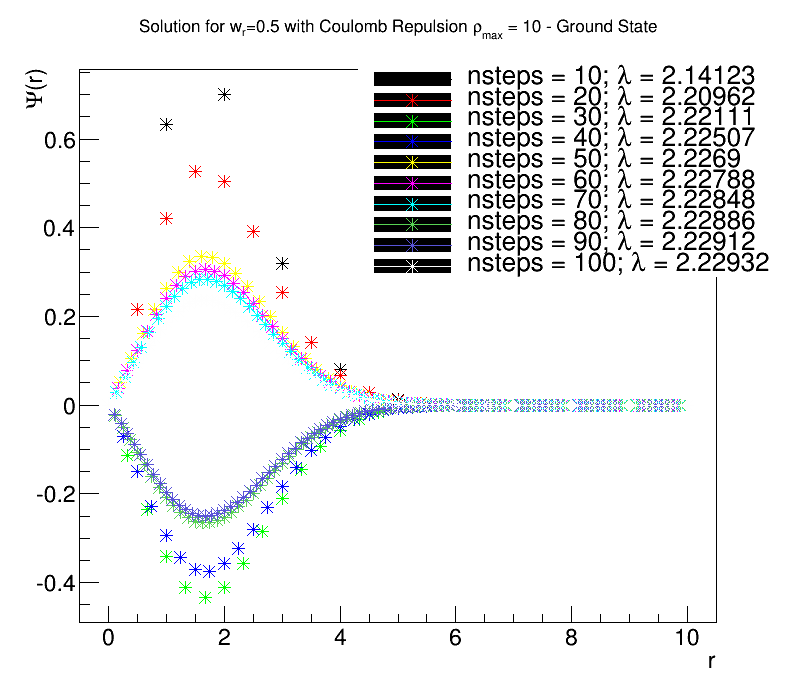
\includegraphics[width=0.45\textwidth]{plots/wr05C10}
\end{subfigure}
\begin{subfigure}
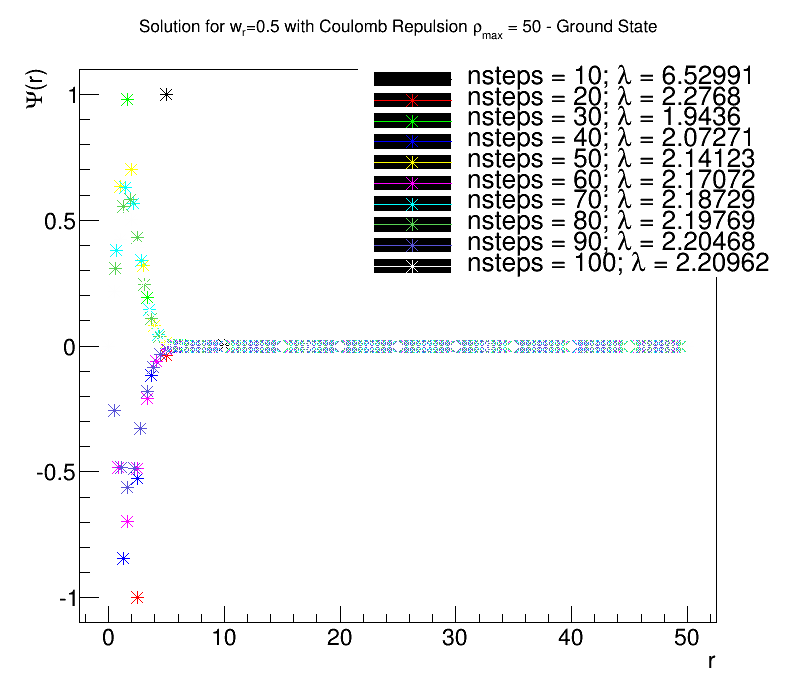
\includegraphics[width=0.45\textwidth]{plots/wr05C50}
\end{subfigure}
\begin{subfigure}
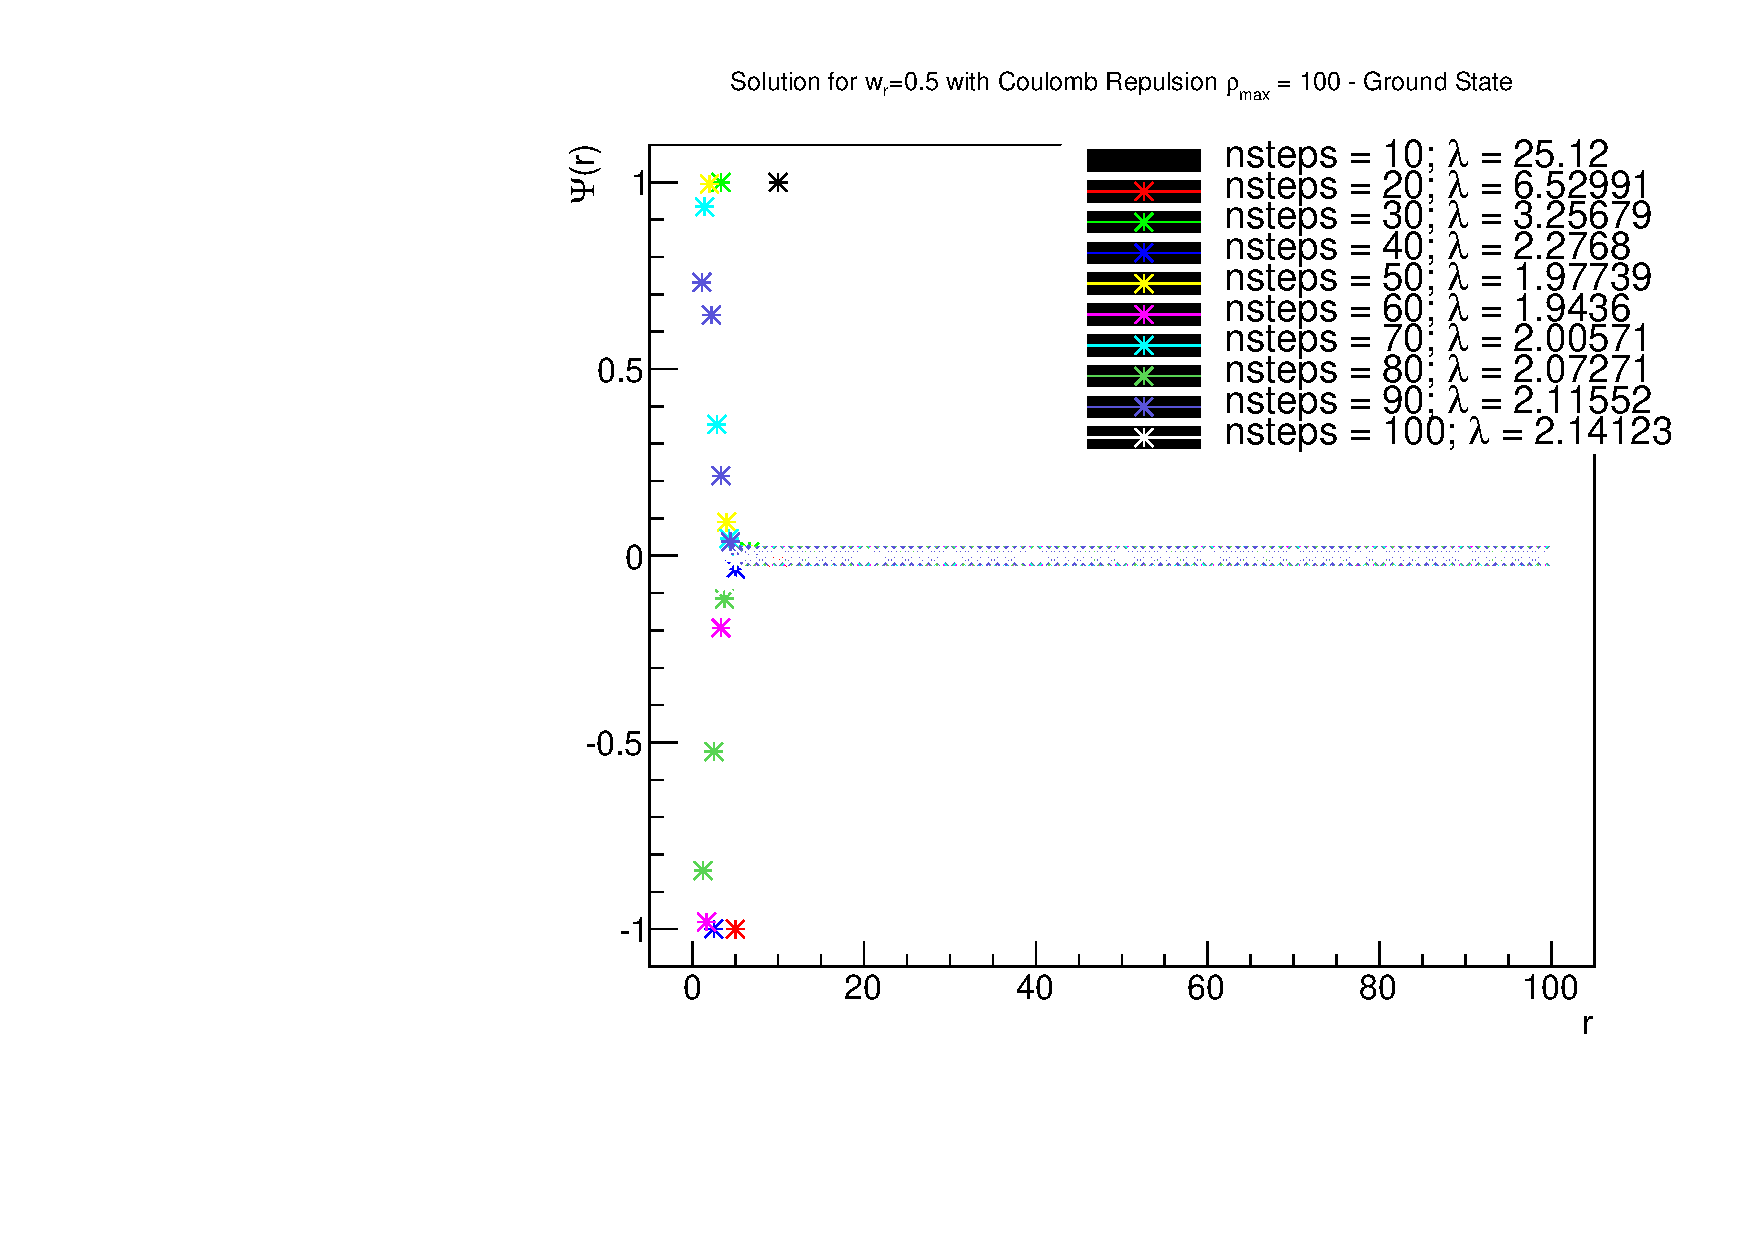
\includegraphics[width=0.45\textwidth]{plots/wr05C100}
\end{subfigure}
\caption{Solutions for the interacting two-electron system for various values of $\rho_{max}$ in the ground state for $\omega_{r}=0.5$.}
\end{center}
\end{figure}

\begin{figure}[h]
\label{fig:2ewr1c}
\begin{center}
\begin{subfigure}
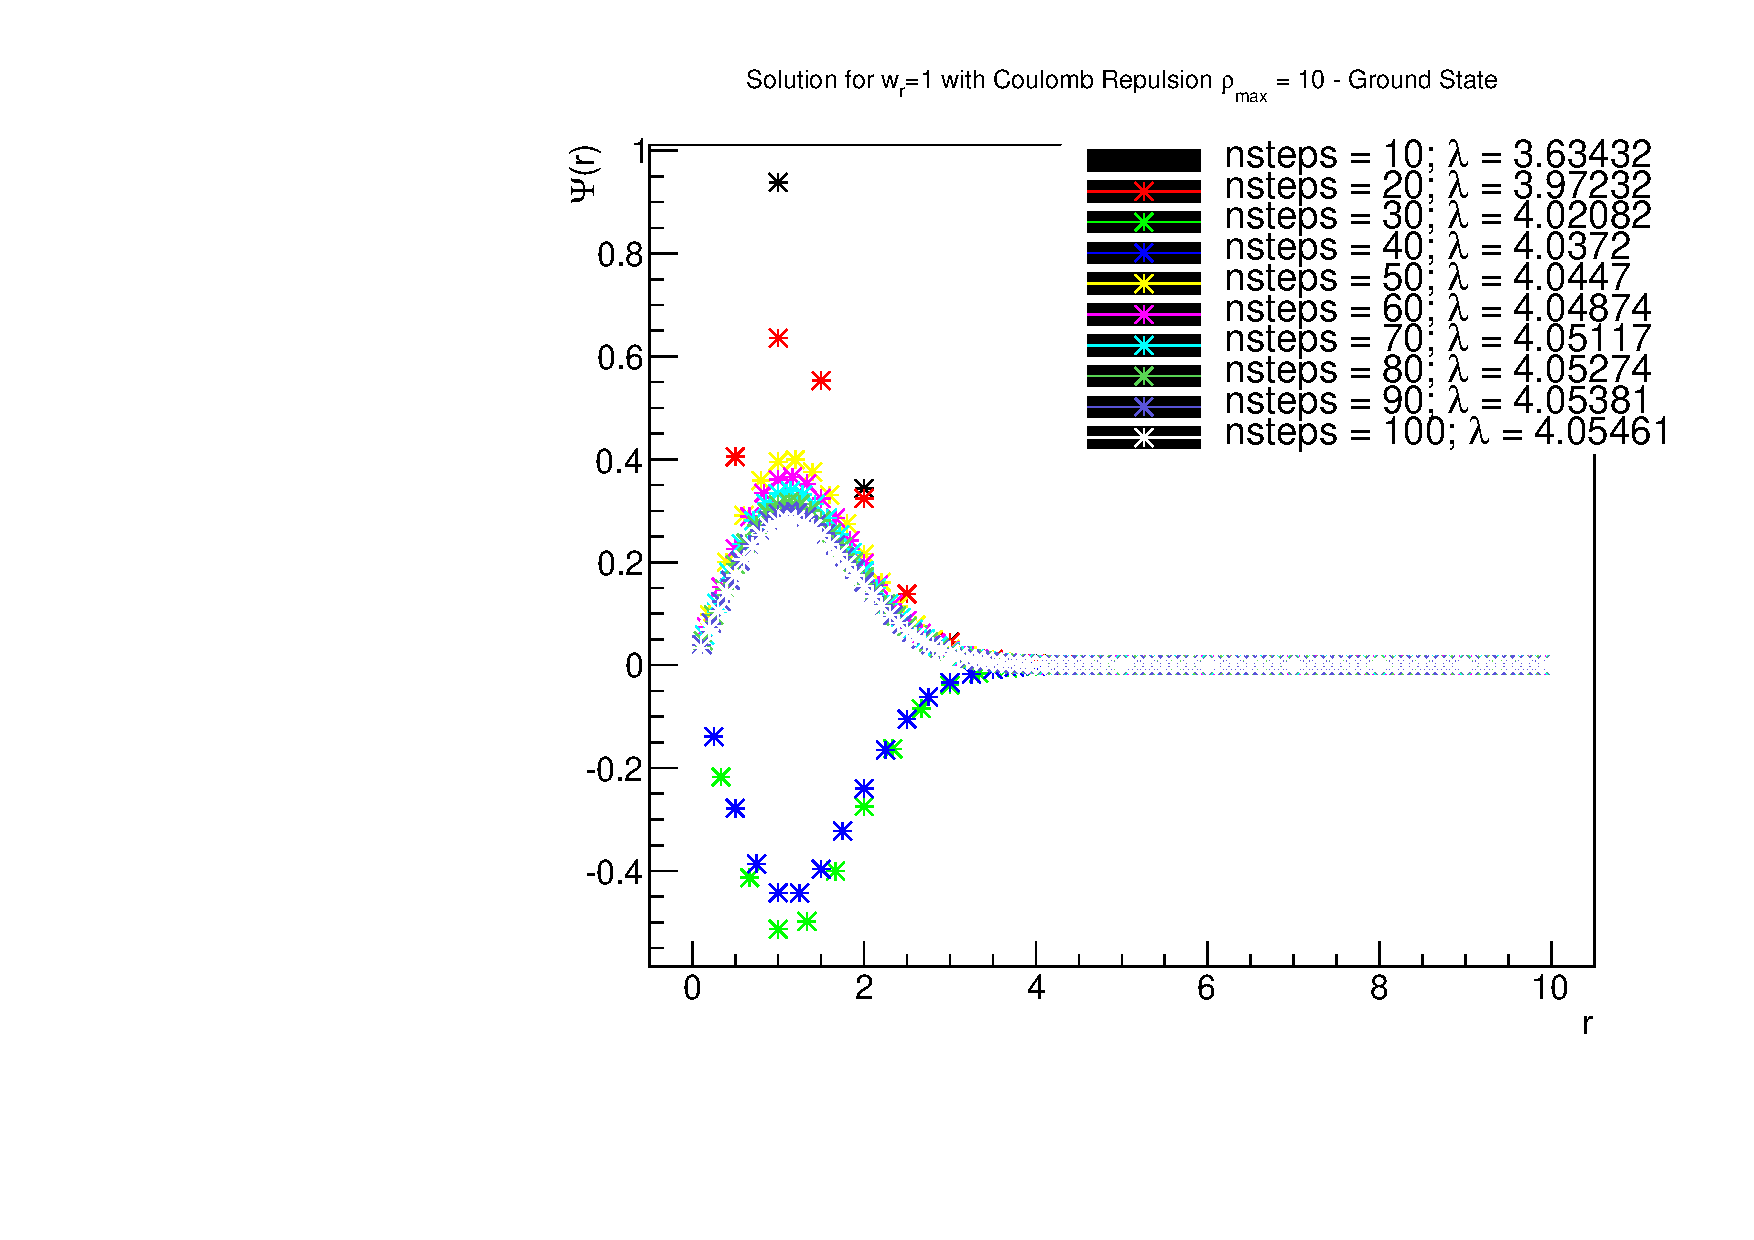
\includegraphics[width=0.45\textwidth]{plots/wr1C10}
\end{subfigure}
\begin{subfigure}
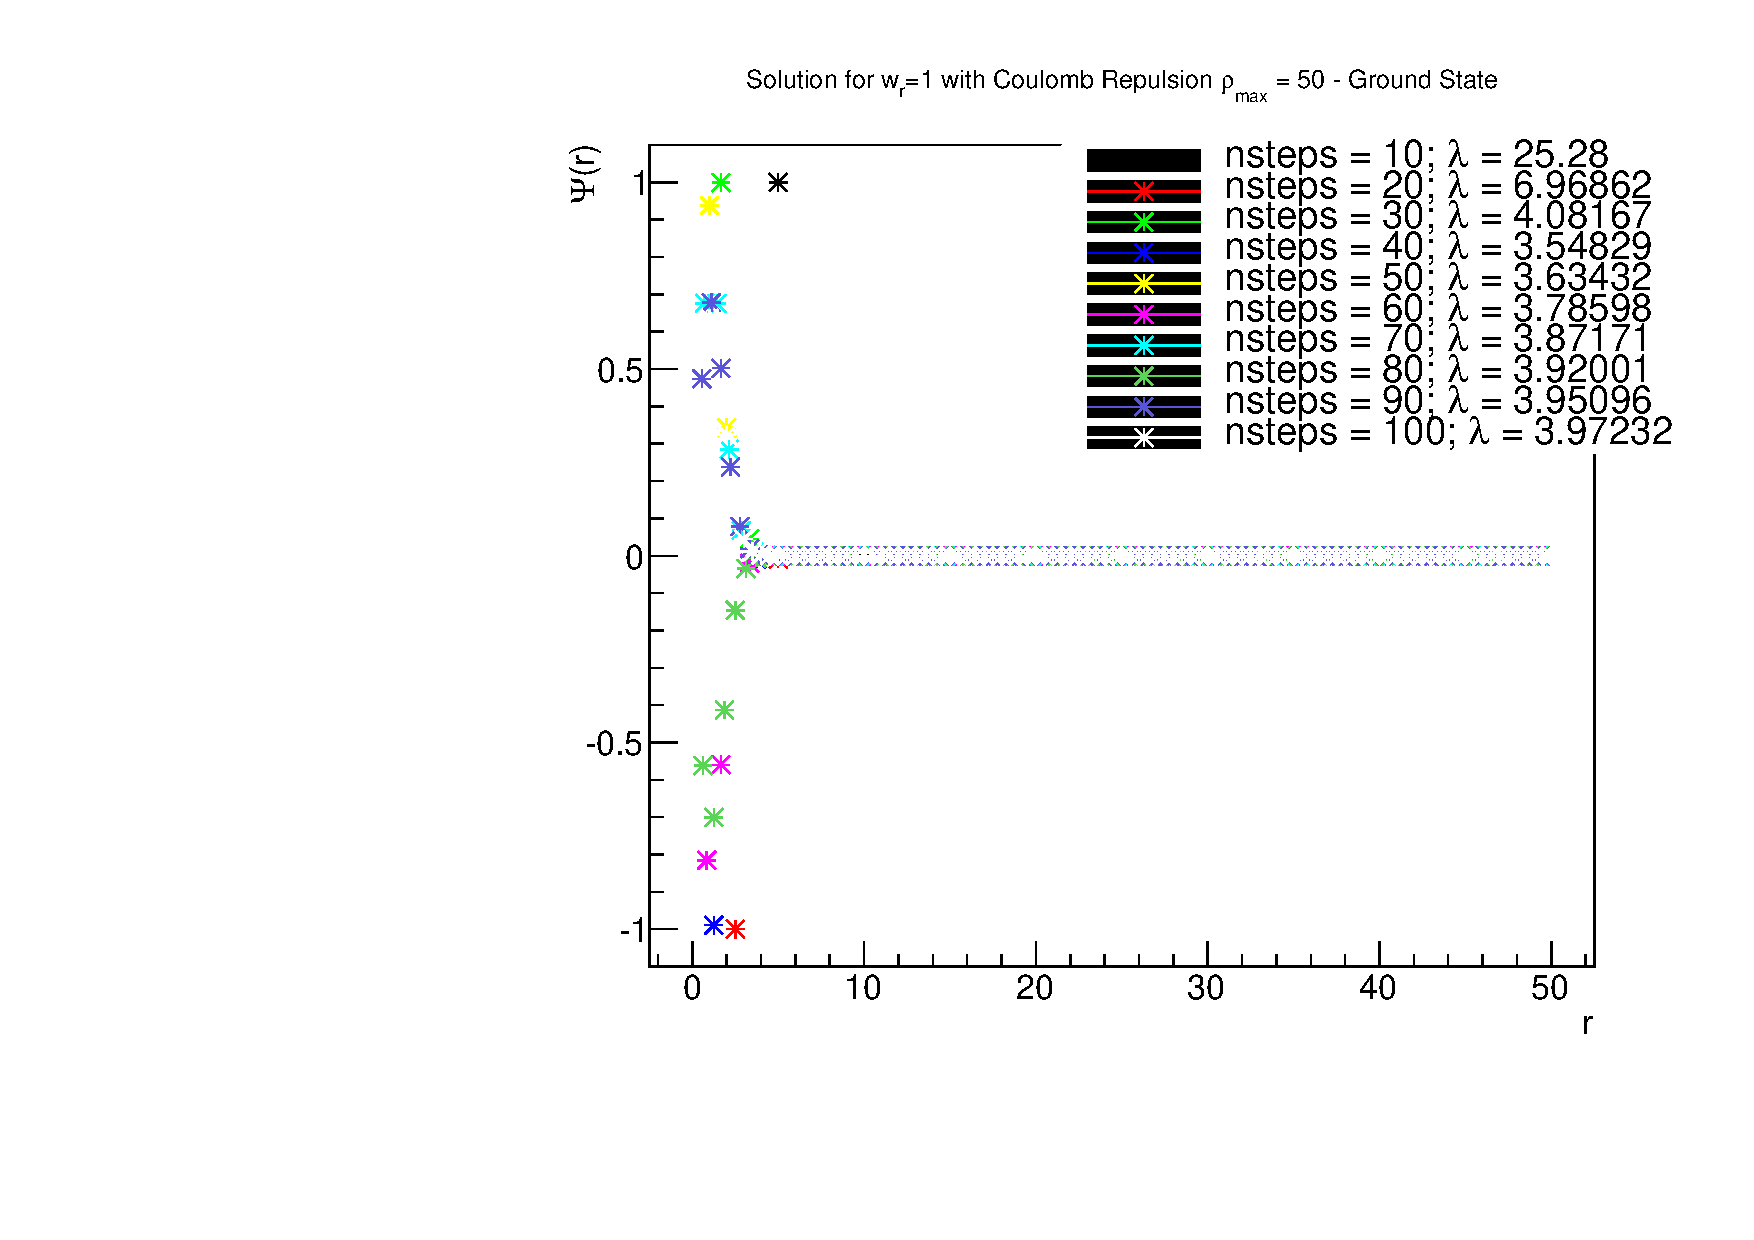
\includegraphics[width=0.45\textwidth]{plots/wr1C50}
\end{subfigure}
\begin{subfigure}
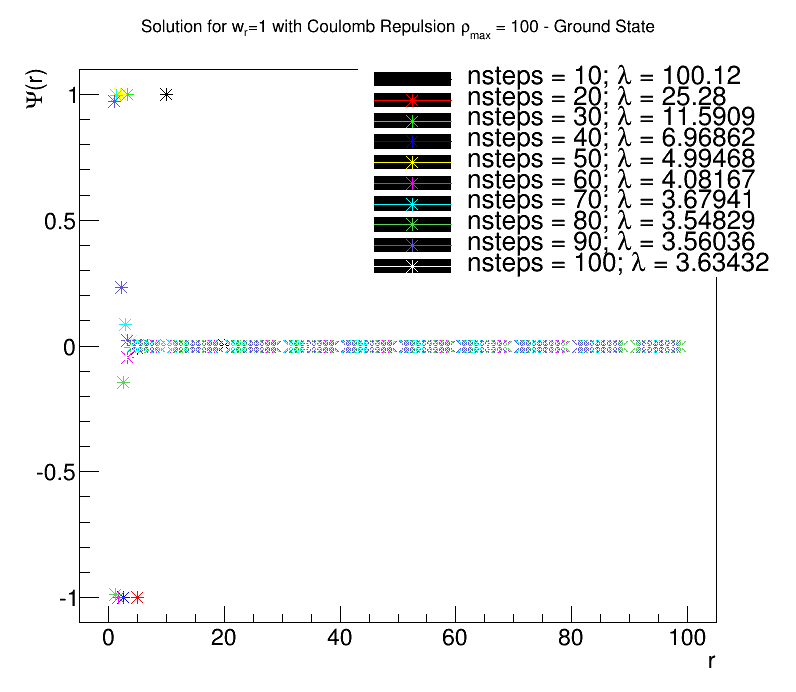
\includegraphics[width=0.45\textwidth]{plots/wr1C100}
\end{subfigure}
\caption{Solutions for the interacting two-electron system for various values of $\rho_{max}$ in the ground state for $\omega_{r}=1.0$.}
\end{center}
\end{figure}

\begin{figure}[h]
\label{fig:2ewr5c}
\begin{center}
\begin{subfigure}
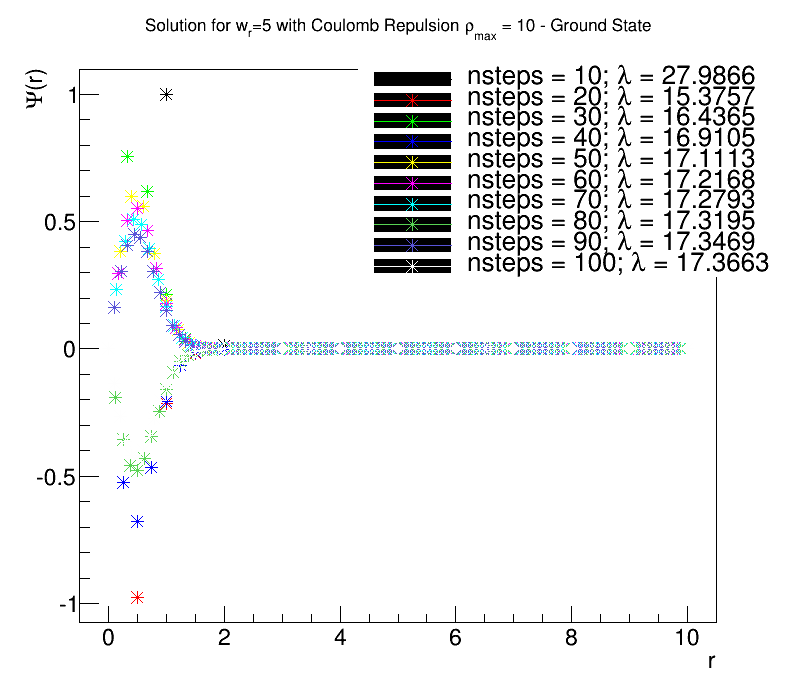
\includegraphics[width=0.45\textwidth]{plots/wr5C10}
\end{subfigure}
\begin{subfigure}
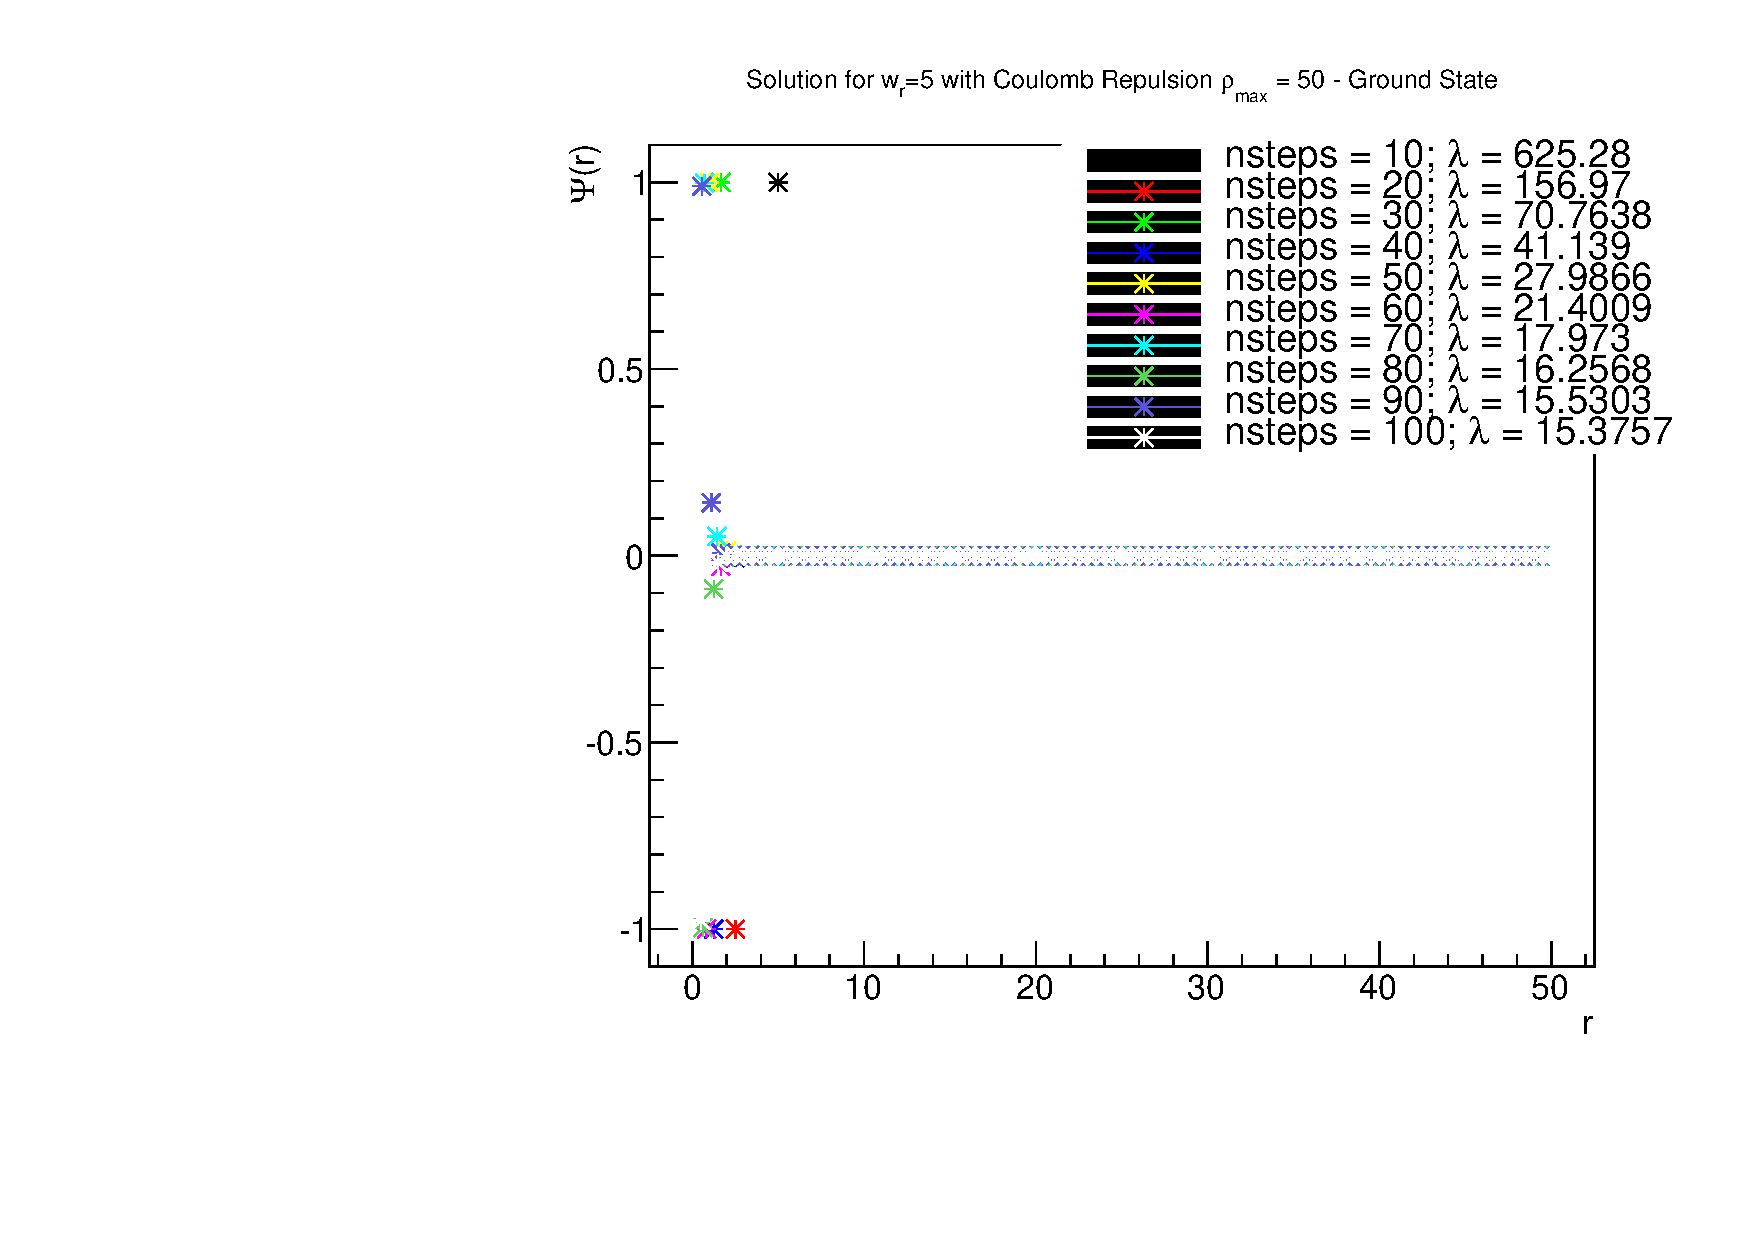
\includegraphics[width=0.45\textwidth]{plots/wr5C50}
\end{subfigure}
\begin{subfigure}
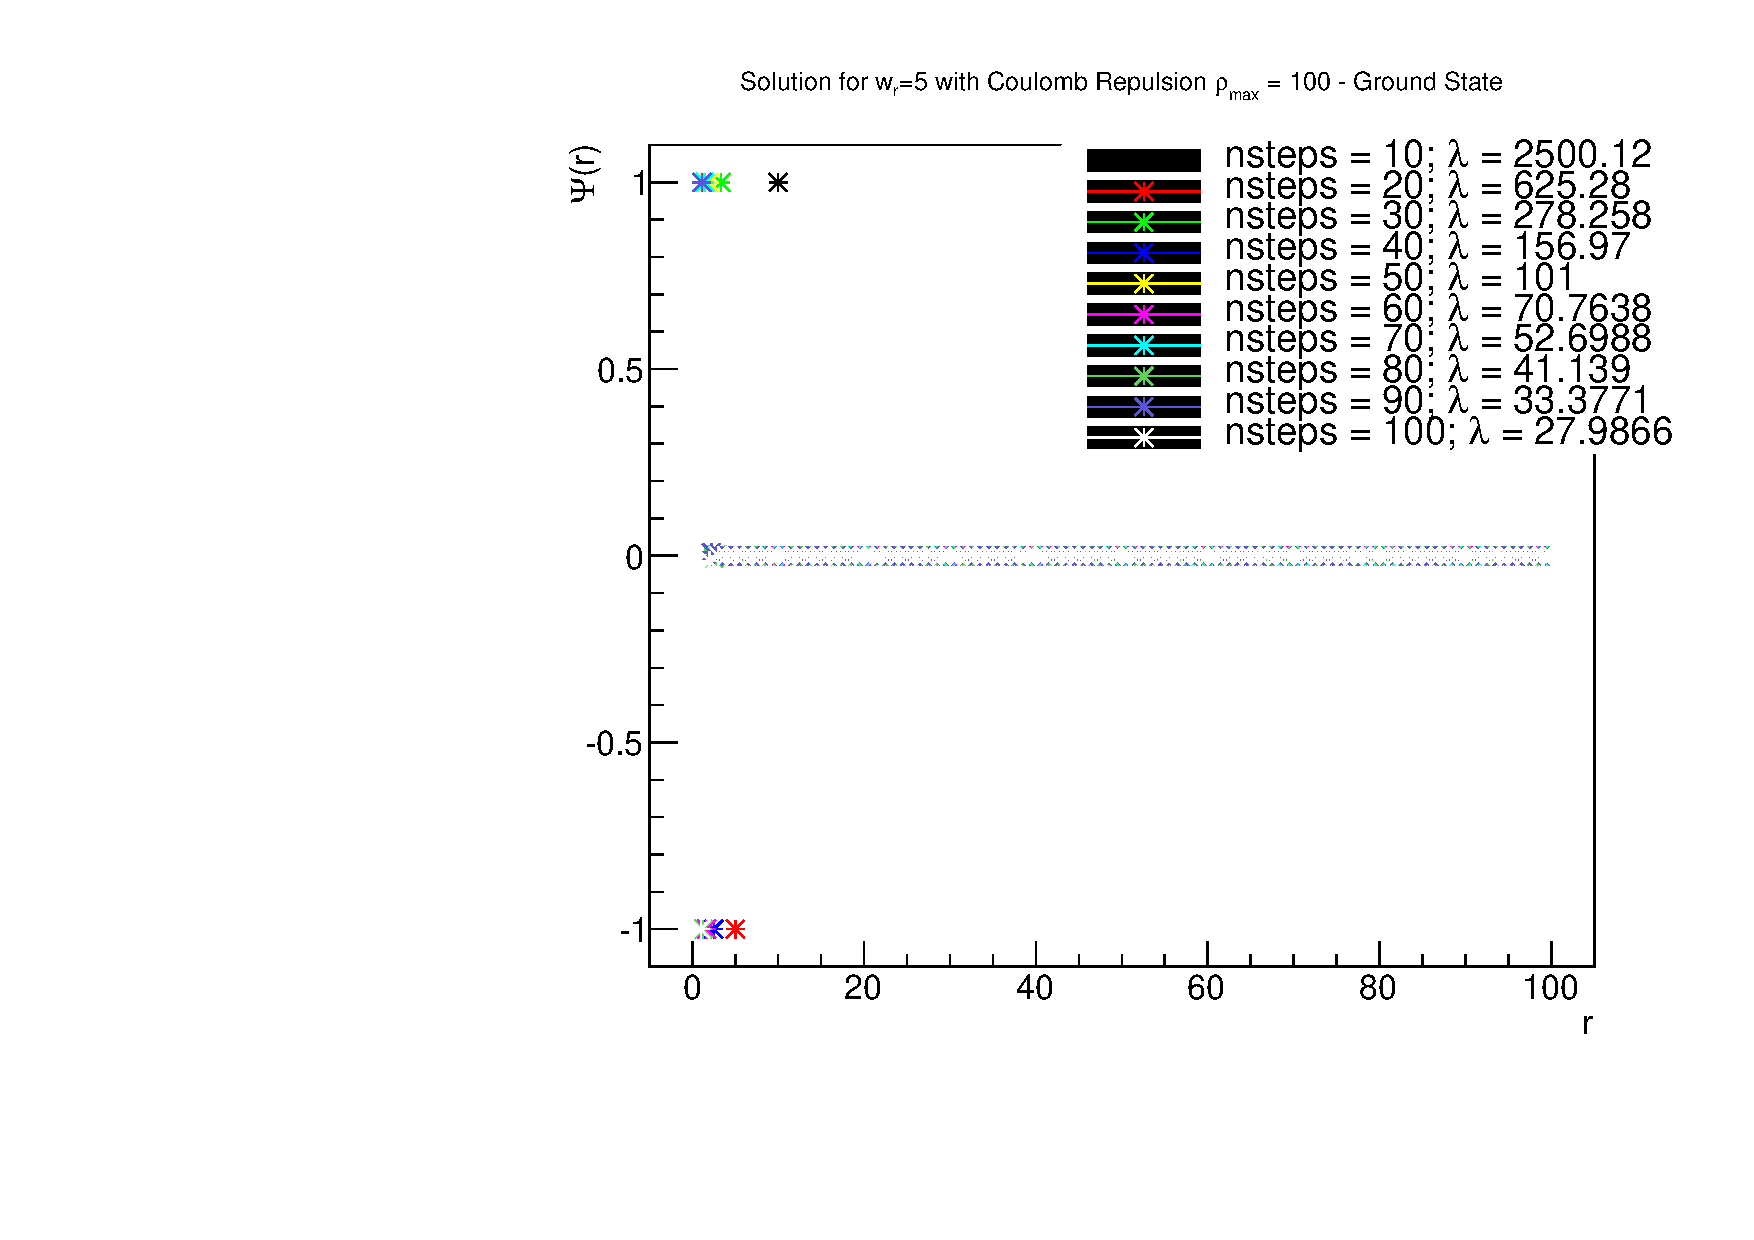
\includegraphics[width=0.45\textwidth]{plots/wr5C100}
\end{subfigure}
\caption{Solutions for the interacting two-electron system for various values of $\rho_{max}$ in the ground state for $\omega_{r}=5.0$.}
\end{center}
\end{figure}

\begin{figure}[h]
\label{fig:2ewr0011}
\begin{center}
\begin{subfigure}
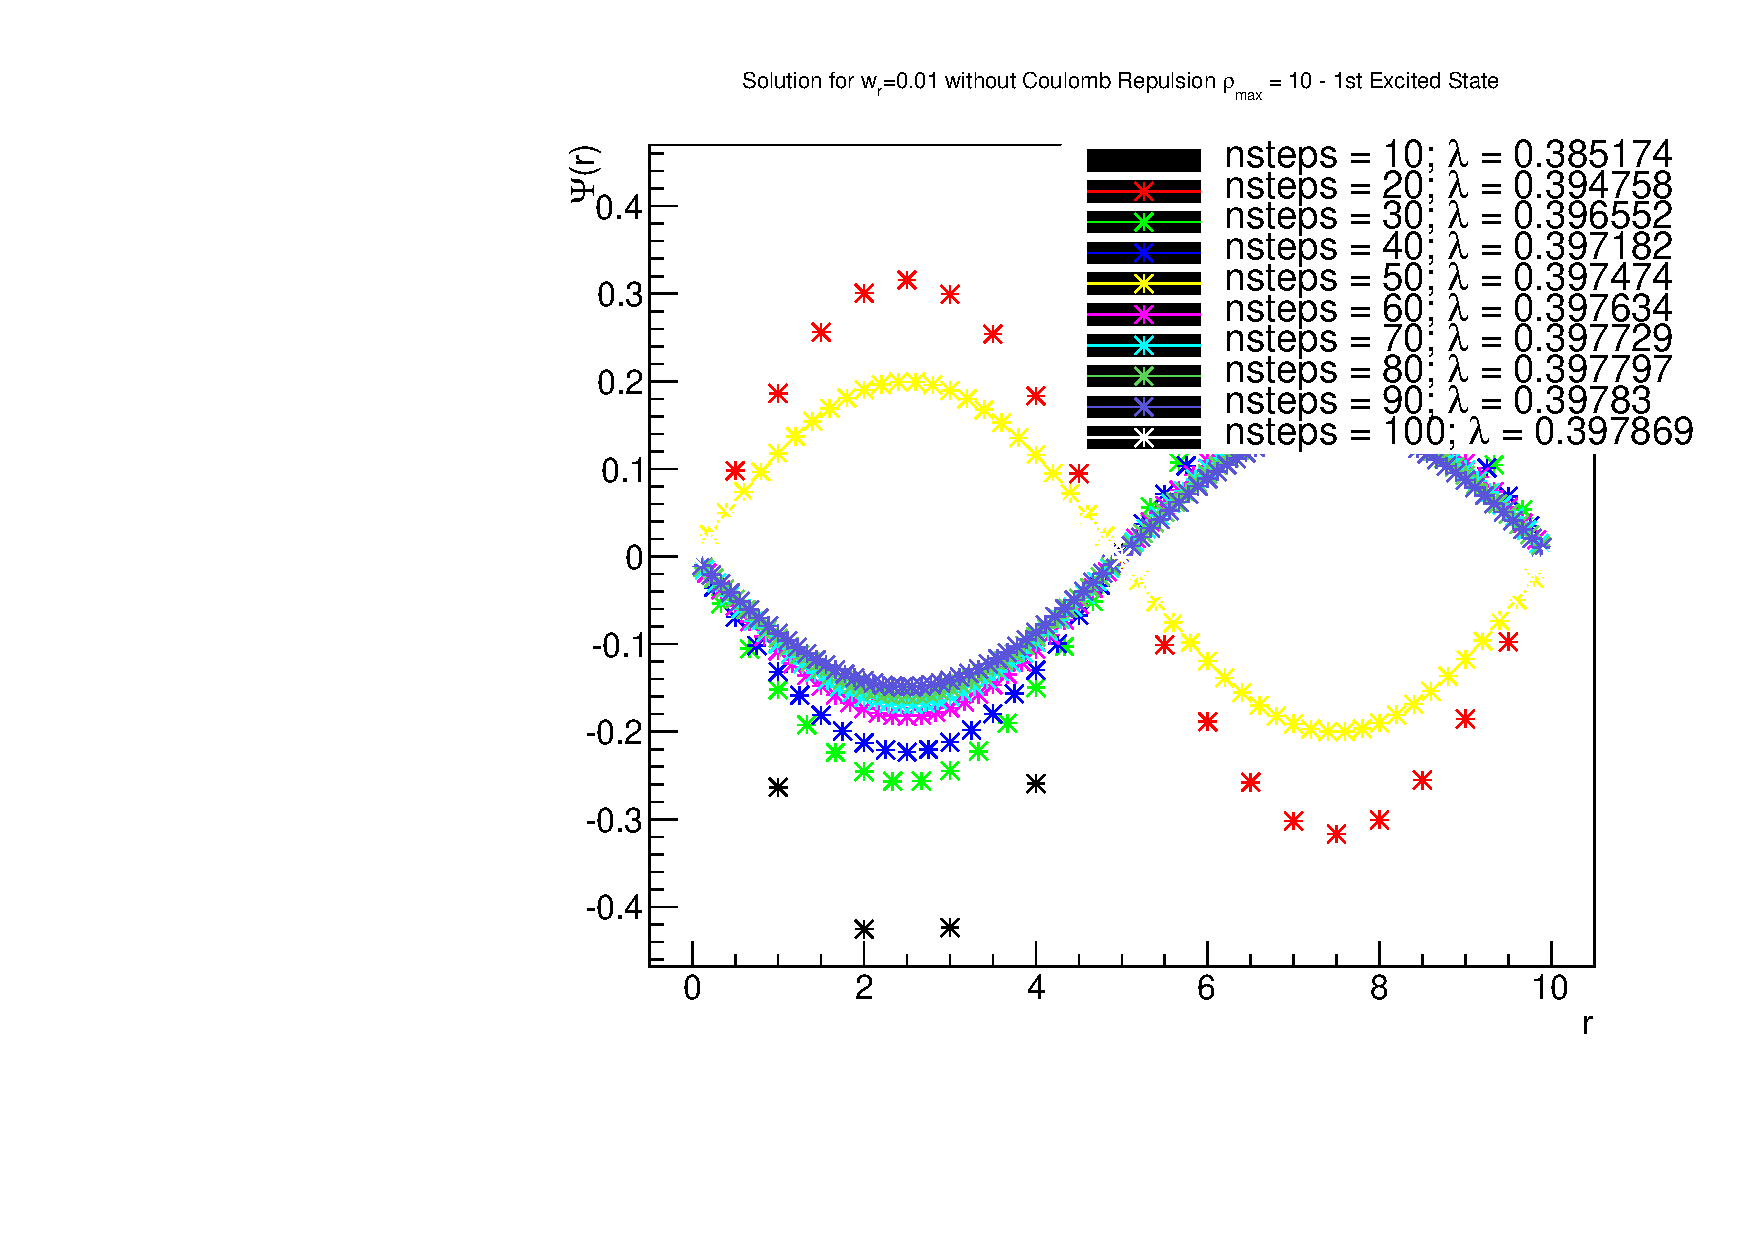
\includegraphics[width=0.45\textwidth]{plots/wr001NC101ststate}
\end{subfigure}
\begin{subfigure}
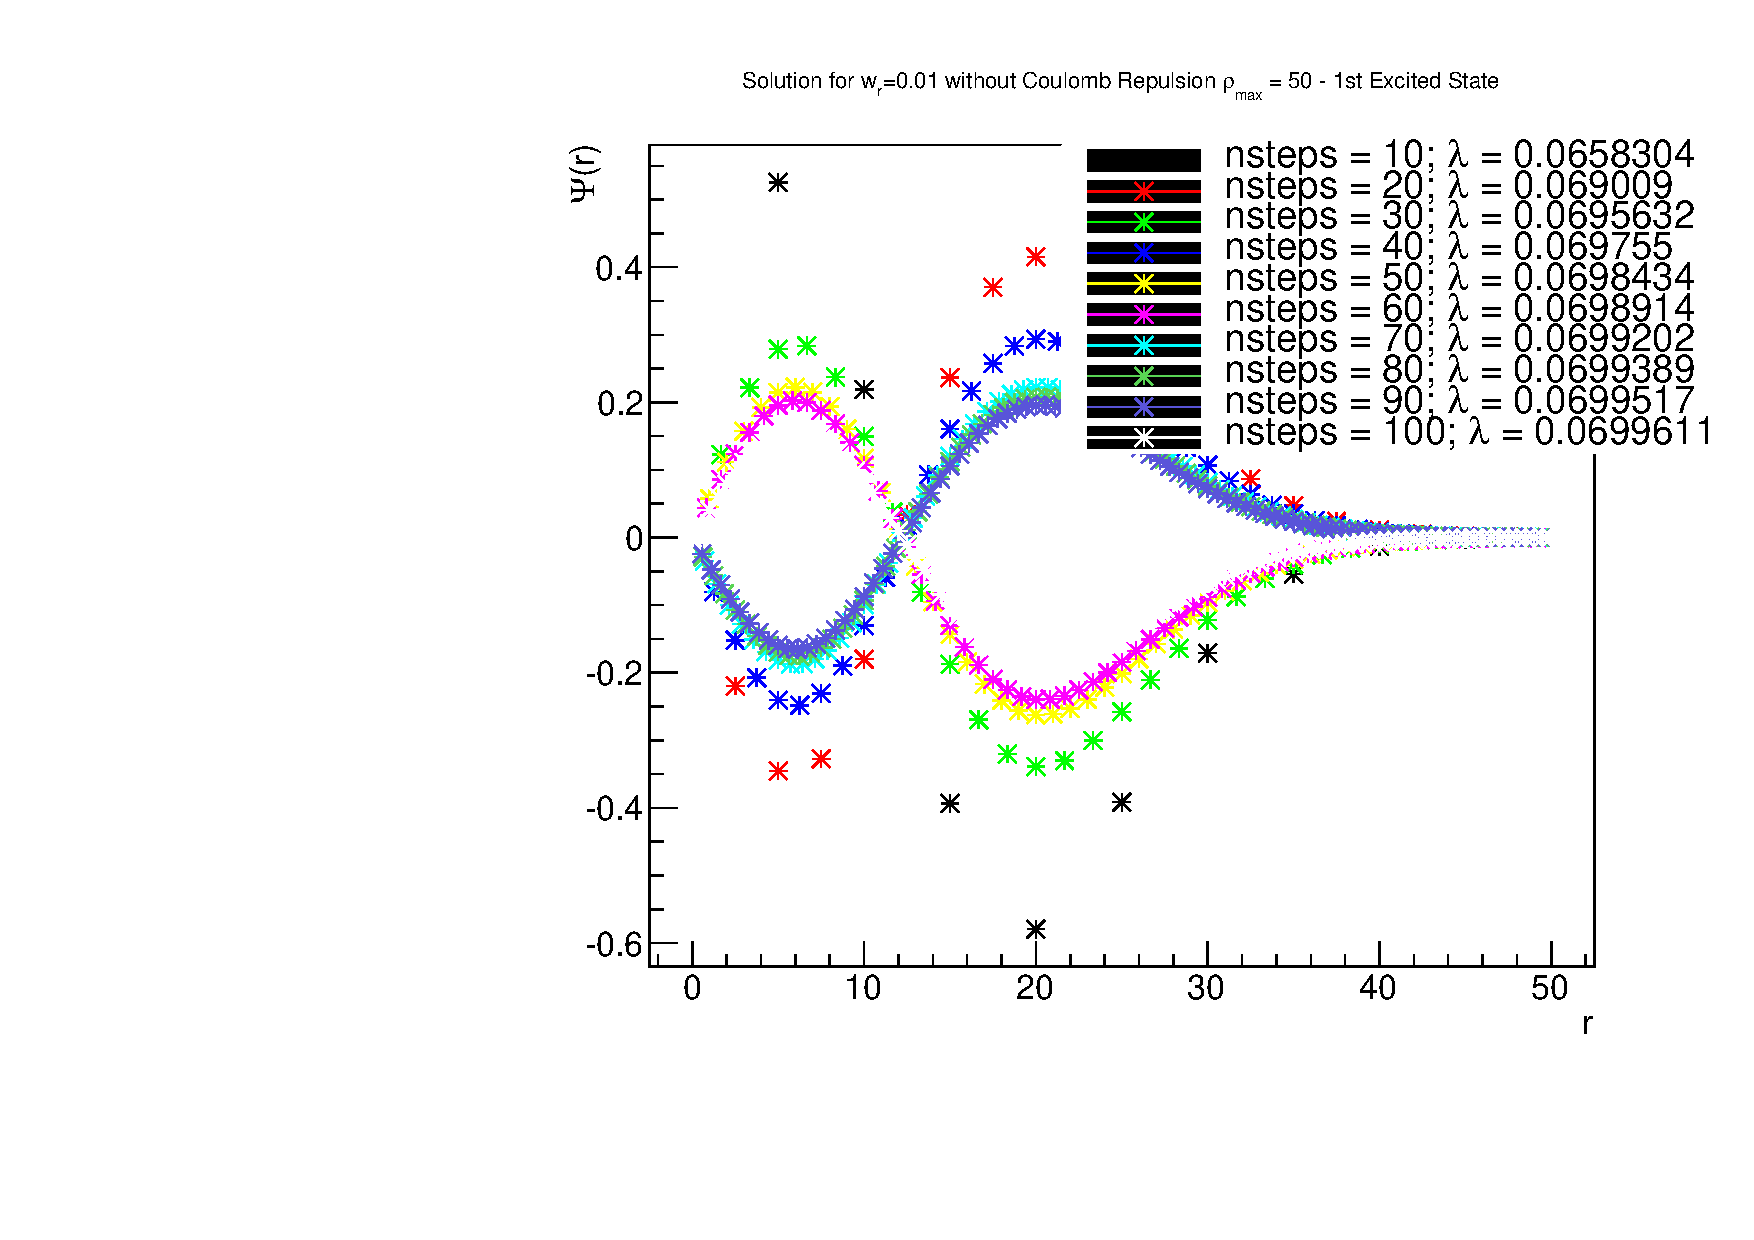
\includegraphics[width=0.45\textwidth]{plots/wr001NC501ststate}
\end{subfigure}
\begin{subfigure}
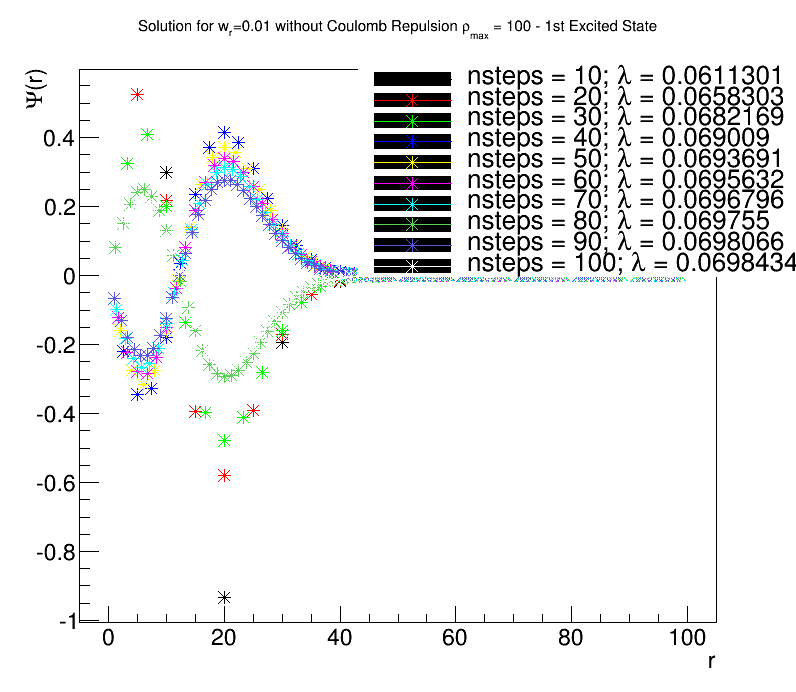
\includegraphics[width=0.45\textwidth]{plots/wr001NC1001ststate}
\end{subfigure}
\caption{Solutions for the non-interacting two-electron system for various values of $\rho_{max}$ in the 1st excited state for $\omega_{r}=0.01$.}
\end{center}
\end{figure}

\begin{figure}[h]
\label{fig:2ewr051}
\begin{center}
\begin{subfigure}
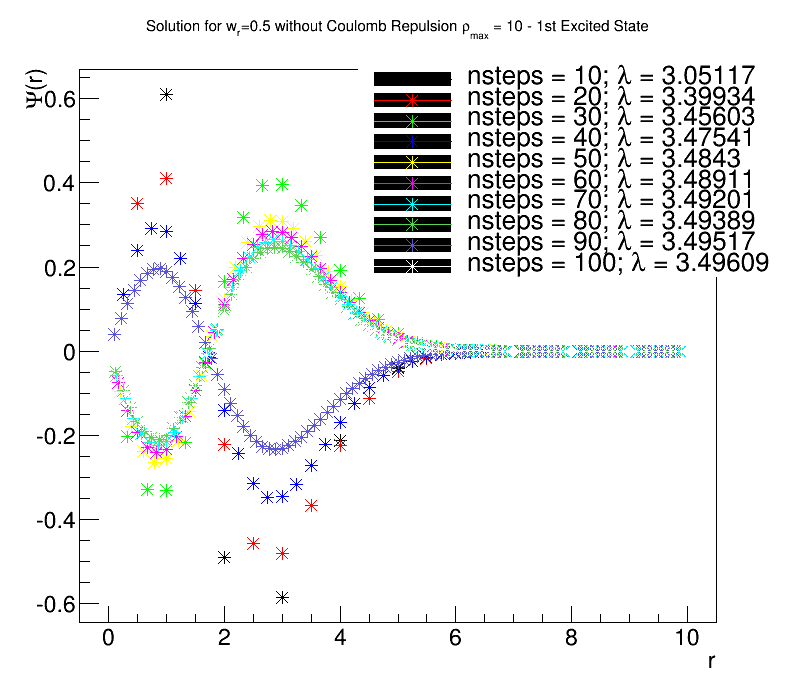
\includegraphics[width=0.45\textwidth]{plots/wr05NC101ststate}
\end{subfigure}
\begin{subfigure}
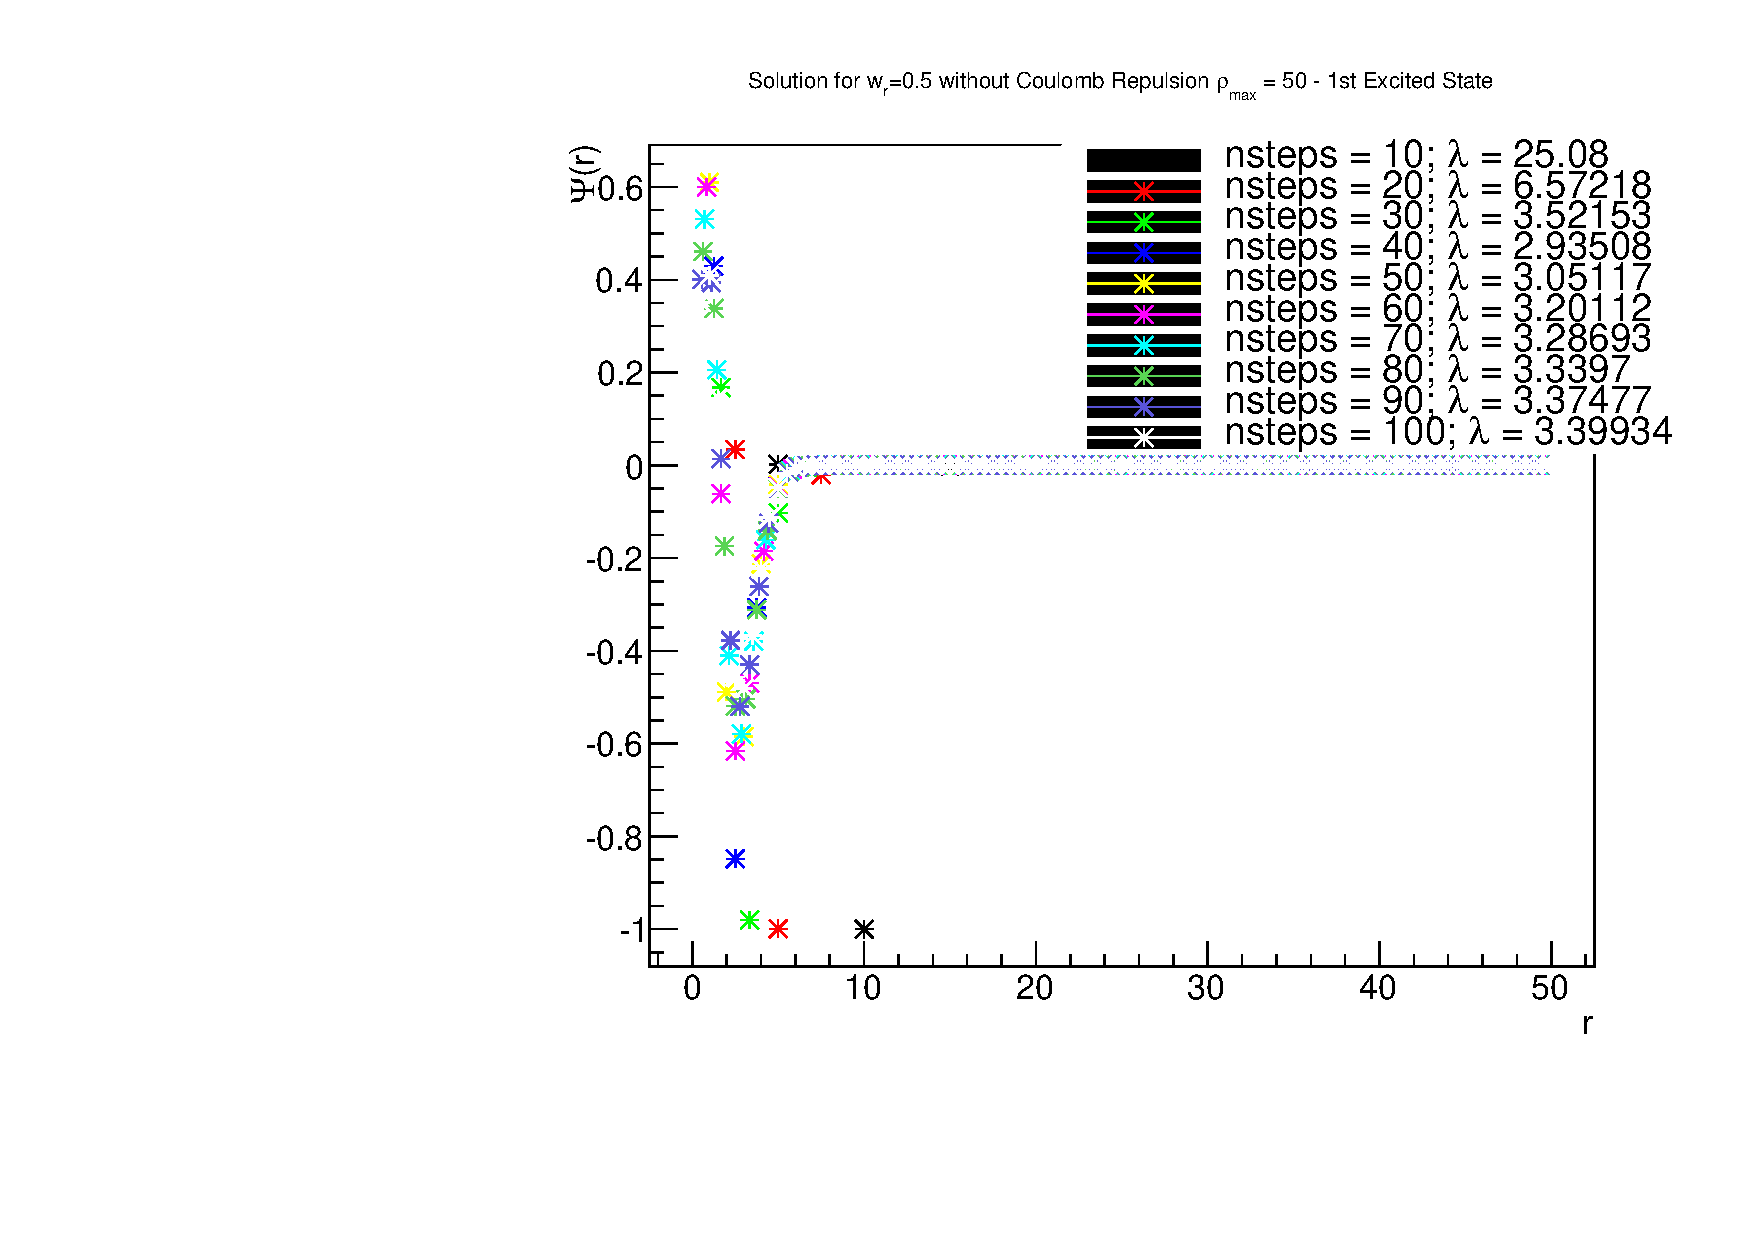
\includegraphics[width=0.45\textwidth]{plots/wr05NC501ststate}
\end{subfigure}
\begin{subfigure}
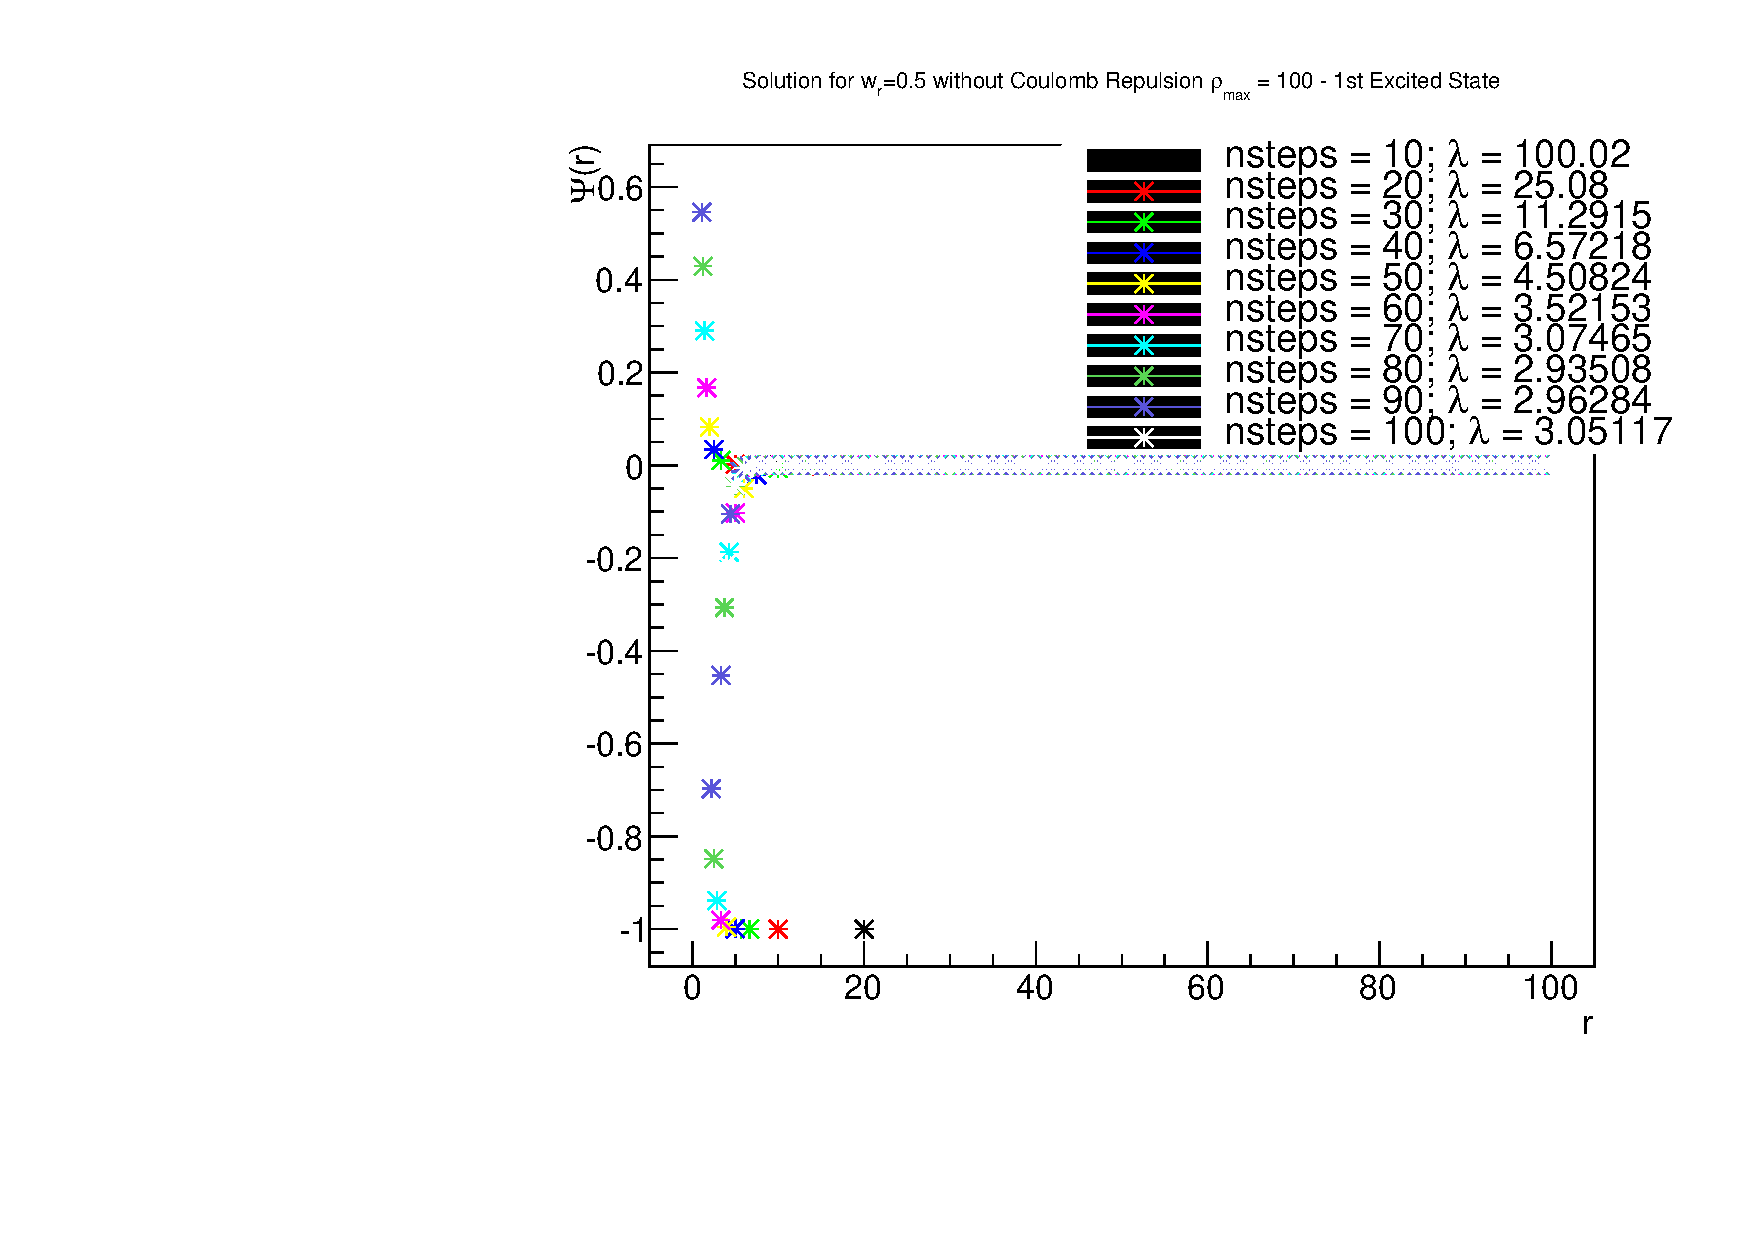
\includegraphics[width=0.45\textwidth]{plots/wr05NC1001ststate}
\end{subfigure}
\caption{Solutions for the non-interacting two-electron system for various values of $\rho_{max}$ in the 1st excited state for $\omega_{r}=0.5$.}
\end{center}
\end{figure}

\begin{figure}[h]
\label{fig:2ewr11}
\begin{center}
\begin{subfigure}
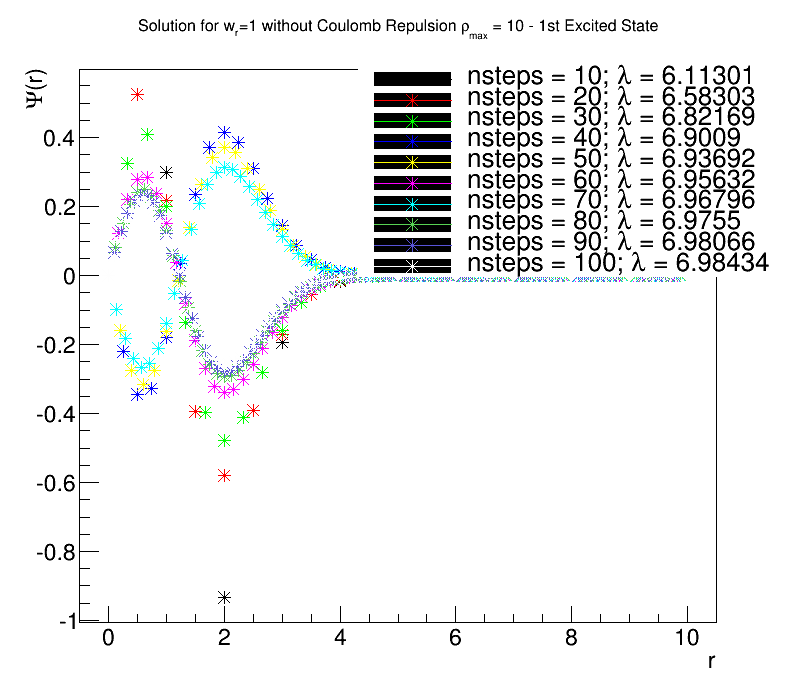
\includegraphics[width=0.45\textwidth]{plots/wr1NC101ststate}
\end{subfigure}
\begin{subfigure}
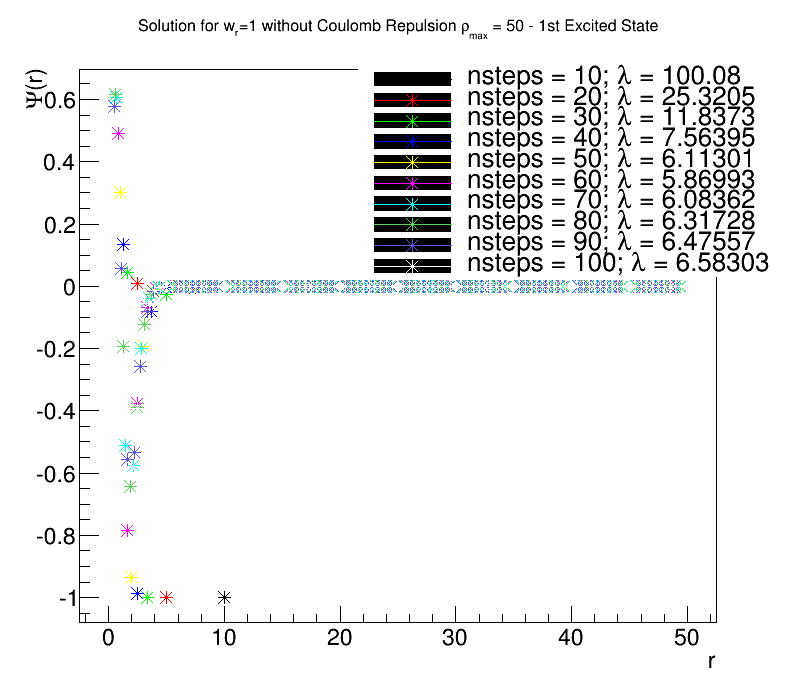
\includegraphics[width=0.45\textwidth]{plots/wr1NC501ststate}
\end{subfigure}
\begin{subfigure}
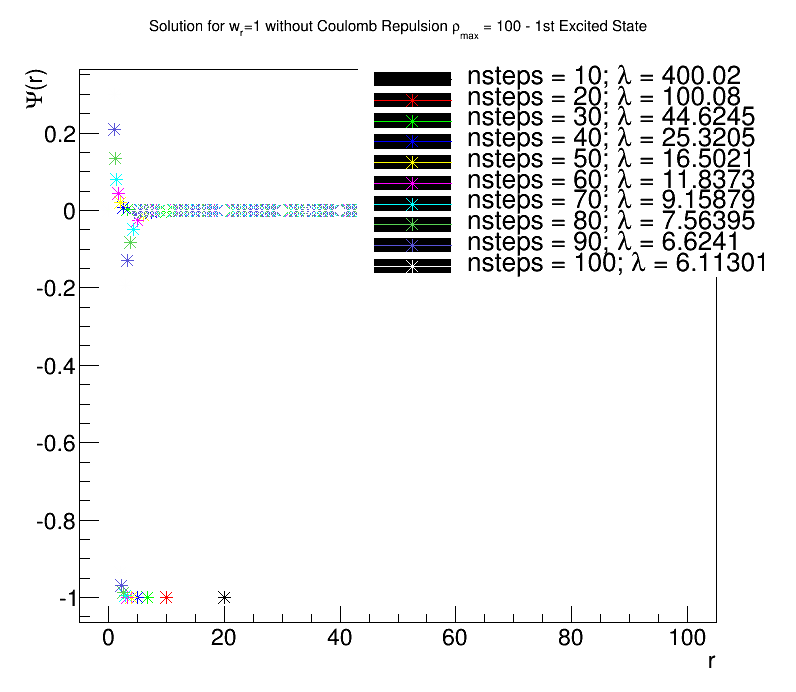
\includegraphics[width=0.45\textwidth]{plots/wr1NC1001ststate}
\end{subfigure}
\caption{Solutions for the non-interacting two-electron system for various values of $\rho_{max}$ in the 1st excited state for $\omega_{r}=1.0$.}
\end{center}
\end{figure}

\begin{figure}[h]
\label{fig:2ewr51}
\begin{center}
\begin{subfigure}
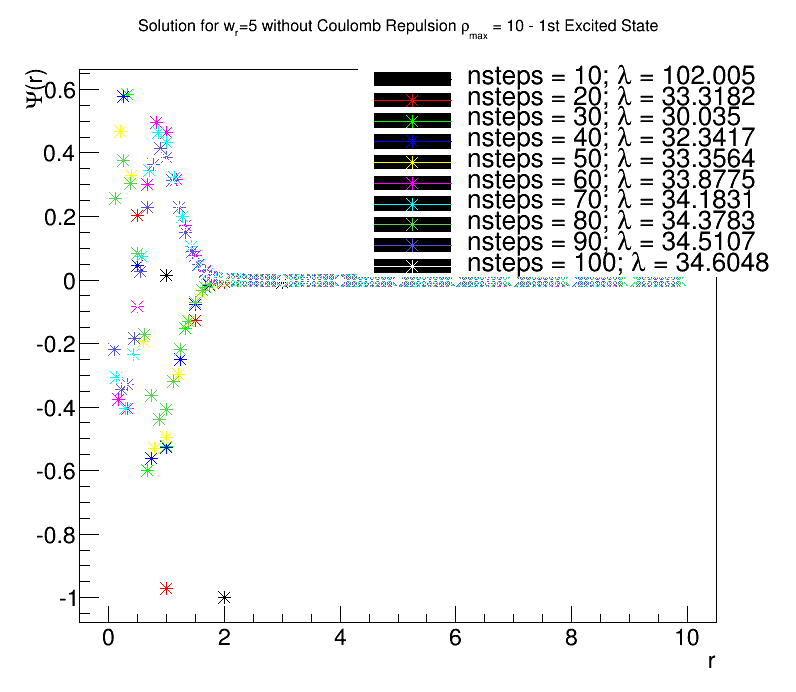
\includegraphics[width=0.45\textwidth]{plots/wr5NC101ststate}
\end{subfigure}
\begin{subfigure}
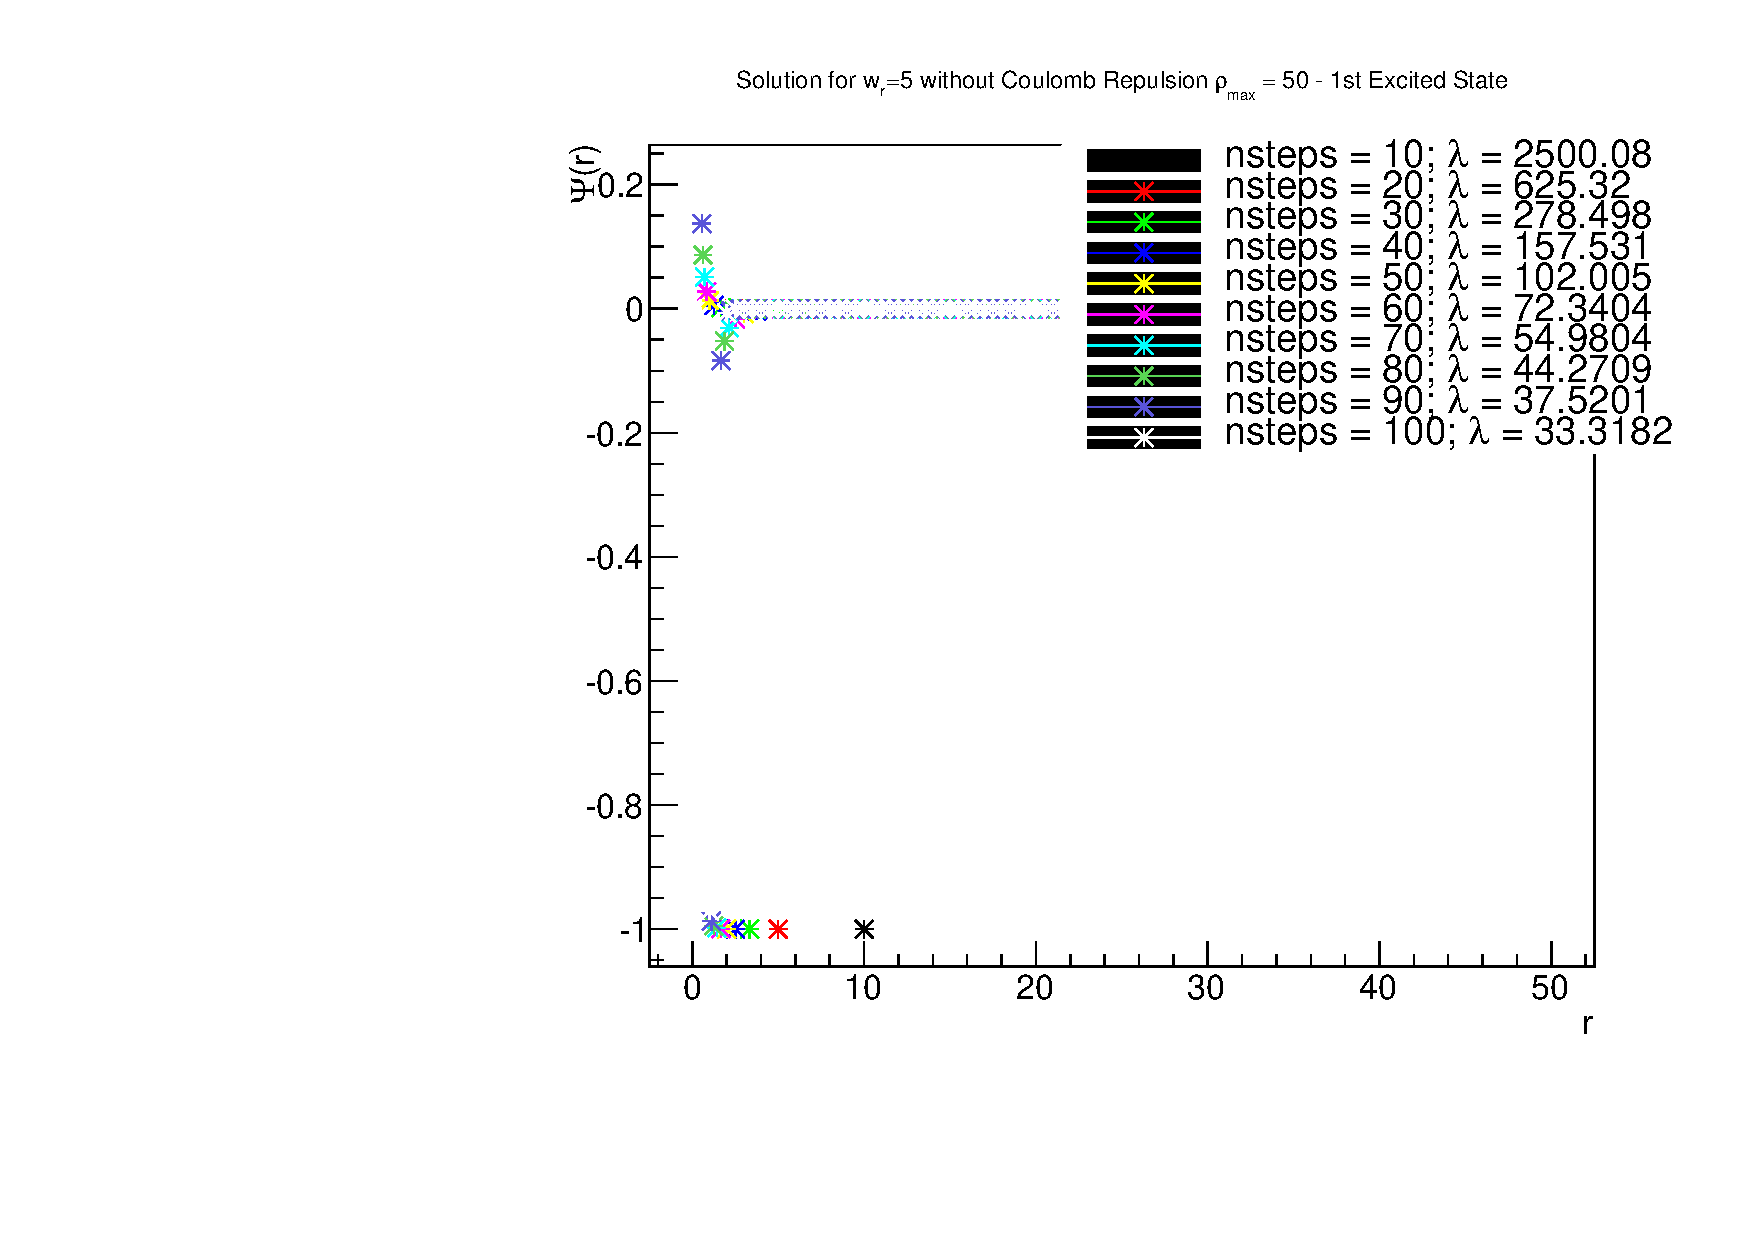
\includegraphics[width=0.45\textwidth]{plots/wr5NC501ststate}
\end{subfigure}
\begin{subfigure}
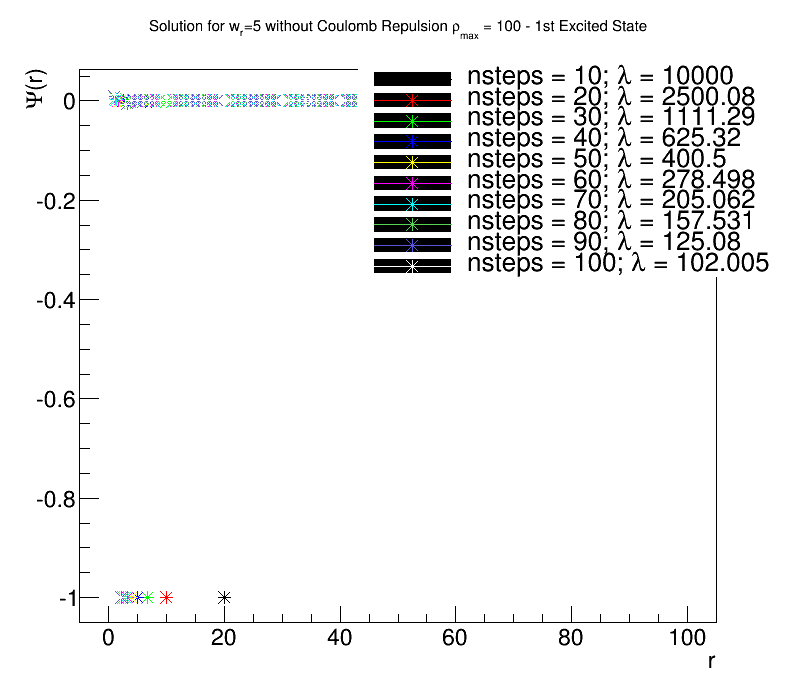
\includegraphics[width=0.45\textwidth]{plots/wr5NC1001ststate}
\end{subfigure}
\caption{Solutions for the non-interacting two-electron system for various values of $\rho_{max}$ in the 1st excited state for $\omega_{r}=5.0$.}
\end{center}
\end{figure}

\begin{figure}[h]
\label{fig:2ewr001c1}
\begin{center}
\begin{subfigure}
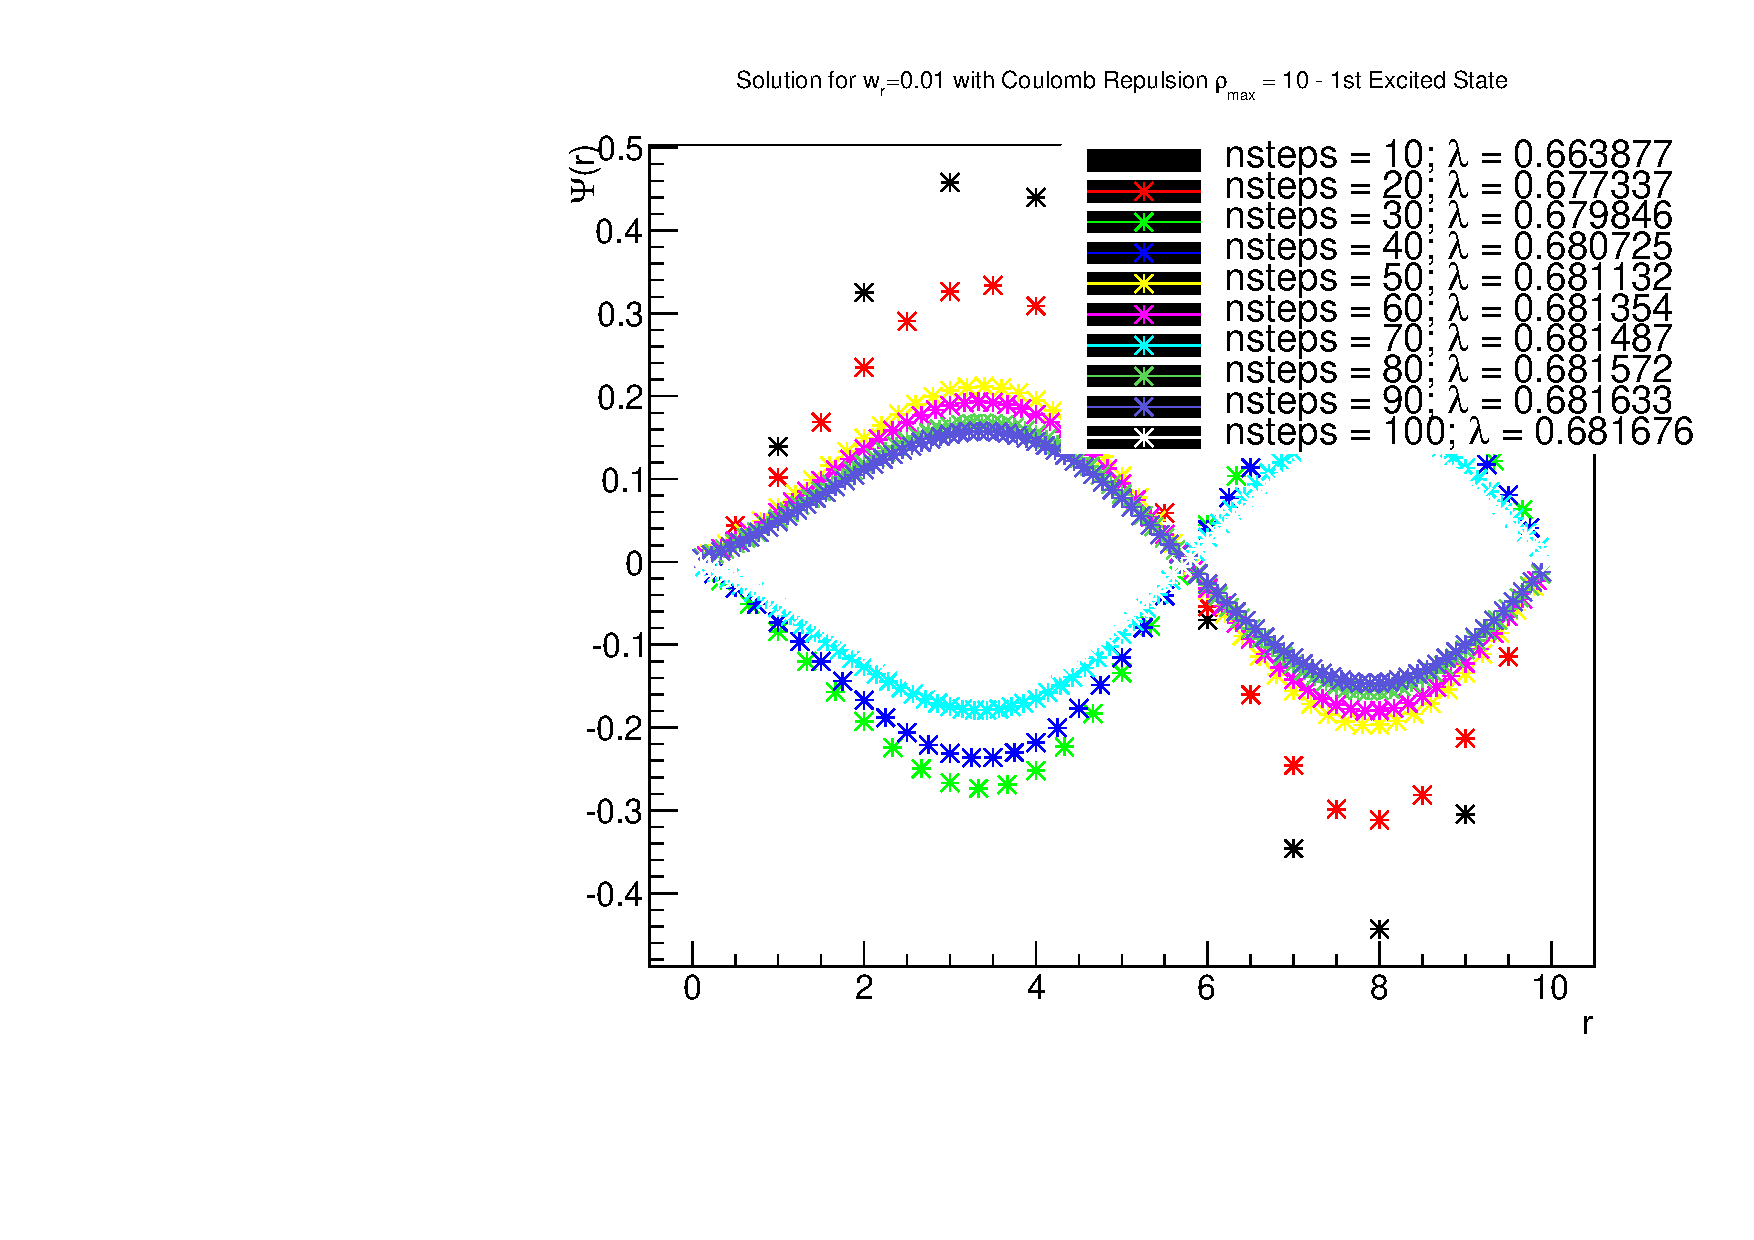
\includegraphics[width=0.45\textwidth]{plots/wr001C101ststate}
\end{subfigure}
\begin{subfigure}
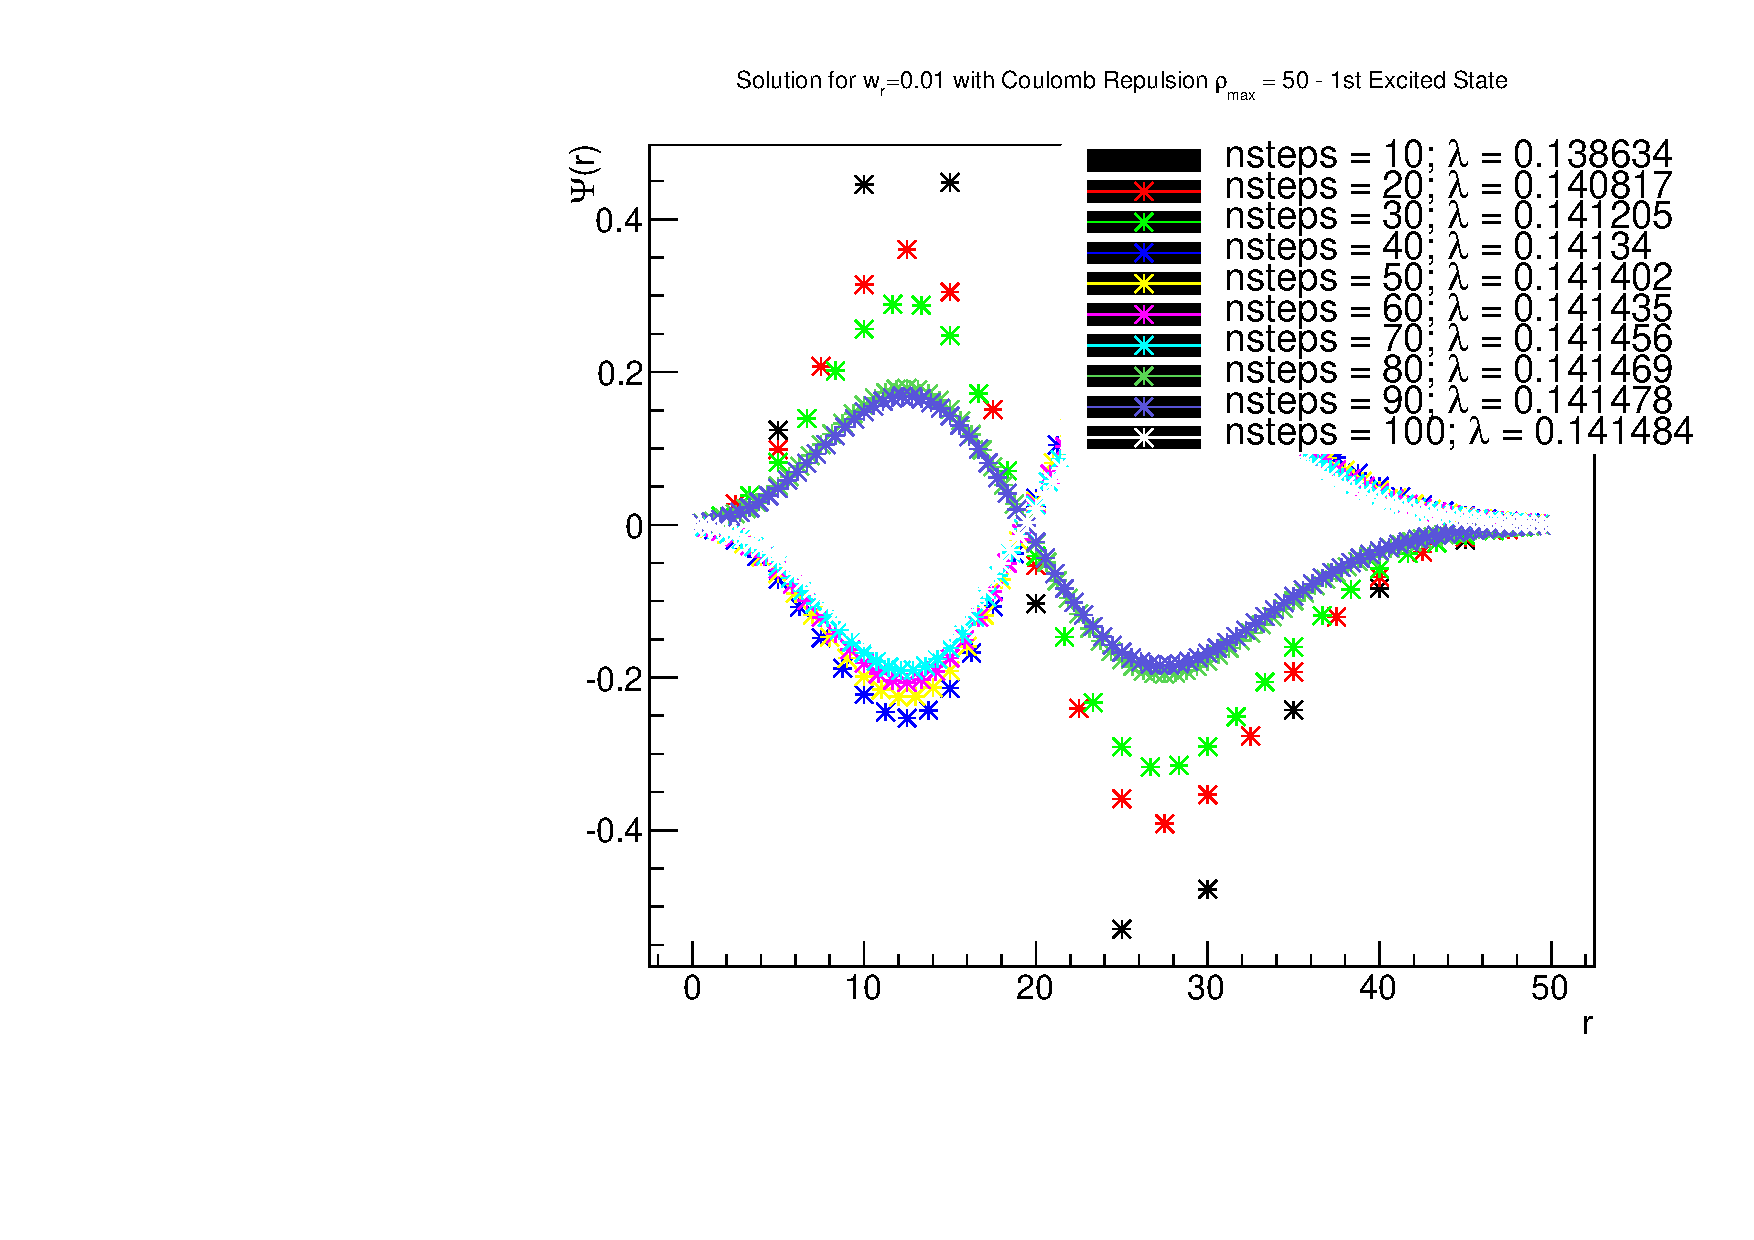
\includegraphics[width=0.45\textwidth]{plots/wr001C501ststate}
\end{subfigure}
\begin{subfigure}
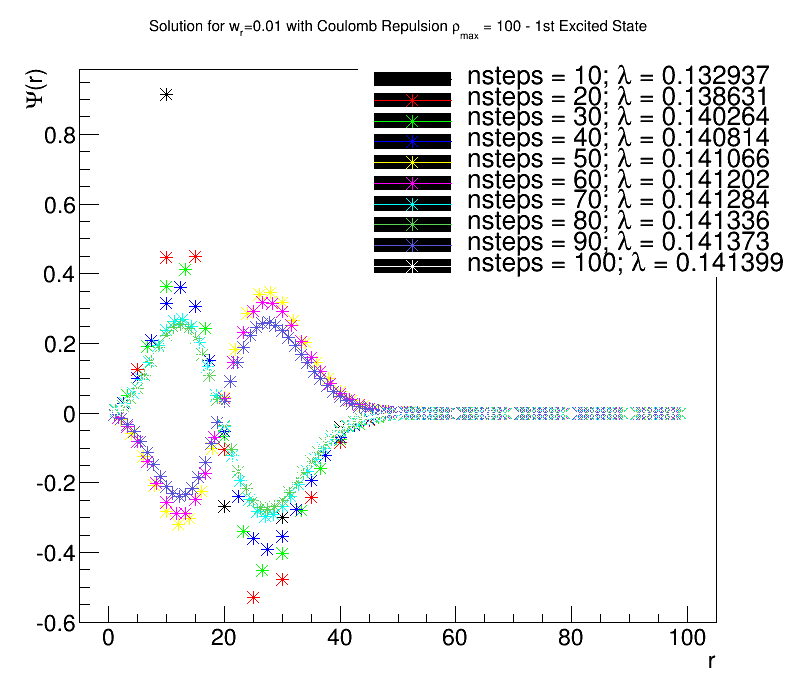
\includegraphics[width=0.45\textwidth]{plots/wr001C1001ststate}
\end{subfigure}
\caption{Solutions for the interacting two-electron system for various values of $\rho_{max}$ in the 1st excited state for $\omega_{r}=0.01$.}
\end{center}
\end{figure}

\begin{figure}[h]
\label{fig:2ewr05c1}
\begin{center}
\begin{subfigure}
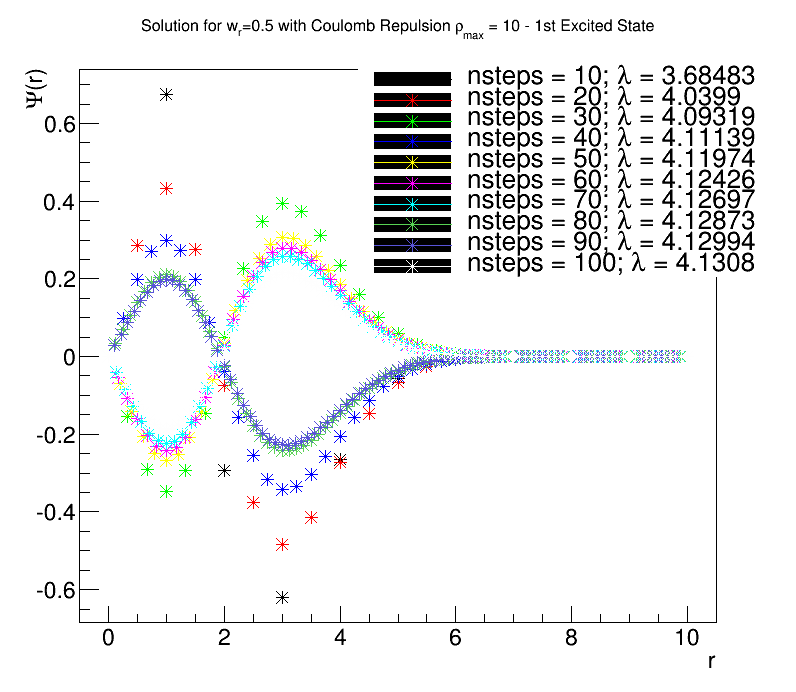
\includegraphics[width=0.45\textwidth]{plots/wr05C101ststate}
\end{subfigure}
\begin{subfigure}
\includegraphics[width=0.45\textwidth]{plots/wr05C501ststate}
\end{subfigure}
\begin{subfigure}
\includegraphics[width=0.45\textwidth]{plots/wr05C1001ststate}
\end{subfigure}
\caption{Solutions for the interacting two-electron system for various values of $\rho_{max}$ in the 1st excited state for $\omega_{r}=0.5$.}
\end{center}
\end{figure}

\begin{figure}[h]
\label{fig:2ewr1c1}
\begin{center}
\begin{subfigure}
\includegraphics[width=0.45\textwidth]{plots/wr1C101ststate}
\end{subfigure}
\begin{subfigure}
\includegraphics[width=0.45\textwidth]{plots/wr1C501ststate}
\end{subfigure}
\begin{subfigure}
\includegraphics[width=0.45\textwidth]{plots/wr1C1001ststate}
\end{subfigure}
\caption{Solutions for the interacting two-electron system for various values of $\rho_{max}$ in the 1st excited state for $\omega_{r}=1.0$.}
\end{center}
\end{figure}

\begin{figure}[h]
\label{fig:2ewr5c1}
\begin{center}
\begin{subfigure}
\includegraphics[width=0.45\textwidth]{plots/wr5C101ststate}
\end{subfigure}
\begin{subfigure}
\includegraphics[width=0.45\textwidth]{plots/wr5C501ststate}
\end{subfigure}
\begin{subfigure}
\includegraphics[width=0.45\textwidth]{plots/wr5C1001ststate}
\end{subfigure}
\caption{Solutions for the interacting two-electron system for various values of $\rho_{max}$ in the 1st excited state for $\omega_{r}=5.0$.}
\end{center}
\end{figure}

\begin{figure}[h]
\label{fig:2ewr0012}
\begin{center}
\begin{subfigure}
\includegraphics[width=0.45\textwidth]{plots/wr001NC102ndstate}
\end{subfigure}
\begin{subfigure}
\includegraphics[width=0.45\textwidth]{plots/wr001NC502ndstate}
\end{subfigure}
\begin{subfigure}
\includegraphics[width=0.45\textwidth]{plots/wr001NC1002ndstate}
\end{subfigure}
\caption{Solutions for the non-interacting two-electron system for various values of $\rho_{max}$ in the 2nd excited state for $\omega_{r}=0.01$.}
\end{center}
\end{figure}

\begin{figure}[h]
\label{fig:2ewr052}
\begin{center}
\begin{subfigure}
\includegraphics[width=0.45\textwidth]{plots/wr05NC102ndstate}
\end{subfigure}
\begin{subfigure}
\includegraphics[width=0.45\textwidth]{plots/wr05NC502ndstate}
\end{subfigure}
\begin{subfigure}
\includegraphics[width=0.45\textwidth]{plots/wr05NC1002ndstate}
\end{subfigure}
\caption{Solutions for the non-interacting two-electron system for various values of $\rho_{max}$ in the 2nd excited state for $\omega_{r}=0.5$.}
\end{center}
\end{figure}

\begin{figure}[h]
\label{fig:2ewr12}
\begin{center}
\begin{subfigure}
\includegraphics[width=0.45\textwidth]{plots/wr1NC102ndstate}
\end{subfigure}
\begin{subfigure}
\includegraphics[width=0.45\textwidth]{plots/wr1NC502ndstate}
\end{subfigure}
\begin{subfigure}
\includegraphics[width=0.45\textwidth]{plots/wr1NC1002ndstate}
\end{subfigure}
\caption{Solutions for the non-interacting two-electron system for various values of $\rho_{max}$ in the 2nd excited state for $\omega_{r}=1.0$.}
\end{center}
\end{figure}

\begin{figure}[h]
\label{fig:2ewr52}
\begin{center}
\begin{subfigure}
\includegraphics[width=0.45\textwidth]{plots/wr5NC102ndstate}
\end{subfigure}
\begin{subfigure}
\includegraphics[width=0.45\textwidth]{plots/wr5NC502ndstate}
\end{subfigure}
\begin{subfigure}
\includegraphics[width=0.45\textwidth]{plots/wr5NC1002ndstate}
\end{subfigure}
\caption{Solutions for the non-interacting two-electron system for various values of $\rho_{max}$ in the 2nd excited state for $\omega_{r}=5.0$.}
\end{center}
\end{figure}

\begin{figure}[h]
\label{fig:2ewr001c2}
\begin{center}
\begin{subfigure}
\includegraphics[width=0.45\textwidth]{plots/wr001C102ndstate}
\end{subfigure}
\begin{subfigure}
\includegraphics[width=0.45\textwidth]{plots/wr001C502ndstate}
\end{subfigure}
\begin{subfigure}
\includegraphics[width=0.45\textwidth]{plots/wr001C1002ndstate}
\end{subfigure}
\caption{Solutions for the interacting two-electron system for various values of $\rho_{max}$ in the 2nd excited state for $\omega_{r}=0.01$.}
\end{center}
\end{figure}

\begin{figure}[h]
\label{fig:2ewr05c2}
\begin{center}
\begin{subfigure}
\includegraphics[width=0.45\textwidth]{plots/wr05C102ndstate}
\end{subfigure}
\begin{subfigure}
\includegraphics[width=0.45\textwidth]{plots/wr05C502ndstate}
\end{subfigure}
\begin{subfigure}
\includegraphics[width=0.45\textwidth]{plots/wr05C1002ndstate}
\end{subfigure}
\caption{Solutions for the interacting two-electron system for various values of $\rho_{max}$ in the 2nd excited state for $\omega_{r}=0.5$.}
\end{center}
\end{figure}

\begin{figure}[h]
\label{fig:2ewr1c2}
\begin{center}
\begin{subfigure}
\includegraphics[width=0.45\textwidth]{plots/wr1C102ndstate}
\end{subfigure}
\begin{subfigure}
\includegraphics[width=0.45\textwidth]{plots/wr1C502ndstate}
\end{subfigure}
\begin{subfigure}
\includegraphics[width=0.45\textwidth]{plots/wr1C1002ndstate}
\end{subfigure}
\caption{Solutions for the interacting two-electron system for various values of $\rho_{max}$ in the 2nd excited state for $\omega_{r}=1.0$.}
\end{center}
\end{figure}

\begin{figure}[h]
\label{fig:2ewr5c2}
\begin{center}
\begin{subfigure}
\includegraphics[width=0.45\textwidth]{plots/wr5C102ndstate}
\end{subfigure}
\begin{subfigure}
\includegraphics[width=0.45\textwidth]{plots/wr5C502ndstate}
\end{subfigure}
\begin{subfigure}
\includegraphics[width=0.45\textwidth]{plots/wr5C1002ndstate}
\end{subfigure}
\caption{Solutions for the interacting two-electron system for various values of $\rho_{max}$ in the 2nd excited state for $\omega_{r}=5.0$.}
\end{center}
\end{figure}

\section{Conclusions}
\label{sec:conclusions}

In the end, a code was developed which was able to successfully reproduce anticipated physics results for the situations of one and two electrons confined to a spherical harmonic oscillator quantum well.  Plots were made which demonstrated the state solutions, and it was shown that the energy eigenvalues converged to the anticipated discretized energy levels.  We were able to use both Householder's Algorithm and Jacobi's Rotation Algorithm in this solution, and determined that the Householder Algorithm was a more efficient tridiagonal solver.
\\\indent However, there were several issues with the code in the end, particularly with the analyzation of the time dependence of the two algorithms.  Several plots did not come out in the anticipated way, indicating that there is a fairly significant bug in \texttt{partb()}.  This does not impact the physics shown or the solutions calculated, but nonetheless it hindered a good description of the coding and the motivation for choosing Householder's Algorithm over Jacobi's.
\\\indent As in Project 1 [2], there are still several upgrades which can and should be made to the \texttt{thevec} and \texttt{themat} classes in \texttt{classes.C}.  These will hopefully be developed in time for Project 3.

\section{Bibliography}
\label{sec:bib}

\begin{enumerate}

\item Brun, Rene, and Fons Rademakers. "ROOT - An Object Oriented Data Analysis Framework." \textit{Nuclear Instruments and Methods in Physics Research A} 389 (1997): 81-86. Web.
\item Drueke, Elizabeth A. \textit{Programming a Linear Algebra Solution to the Poisson Equation.} Rep. N.p.: n.p., n.d. Print.
\item \textit{Lib.cpp.} Program documentation. Numerical Recipes Software, n.d. Web.
\item Hjorth-Jensen, Morten. \textit{Computational Physics}. N.p.: Department of Physics, U of Oslo, n.d. Print.
\item Sakurai, J. J., and San Fu Tuan. Modern Quantum Mechanics. Menlo Park, CA: Benjamin/Cummings, 1985. Print.

\end{enumerate}

\end{document}